\documentclass[]{article}
\usepackage{amsmath}\usepackage{amsfonts}
\usepackage[english]{babel}
\usepackage{amsthm}
\usepackage{listings}
\usepackage{courier}

\usepackage{fancyvrb}
\usepackage{beramono}
\usepackage{mathtools}
\usepackage{hyperref}

\usepackage[usenames,dvipsnames]{xcolor}
\usepackage[T1]{fontenc}
\usepackage[margin=1in,footskip=0.25in]{geometry}  % margin, foot skip
\usepackage[fontsize=12pt]{fontsize}
\usepackage[font=tiny]{caption}
\usepackage{wrapfig}
\usepackage{float}
\usepackage[final]{graphicx}


\lstset{basicstyle=\footnotesize\ttfamily,breaklines=true}
\newcommand{\indep}{\perp \!\!\! \perp}
\graphicspath{{.}}
\theoremstyle{definition}
\newtheorem{theorem}{Theorem}            % Theorem counter global 
\newtheorem{prop}{Proposition}[section]  % proposition counter is section
\newtheorem{lemma}{Lemma}[subsection]    % lemma counter is subsection
\newtheorem{definition}{Definition}      % theorem counter is global
\newtheorem{remark}{Remark}[subsection]  % remark counter is subsection
\hypersetup{
    colorlinks=true,
    linkcolor=blue,
    filecolor=magenta,
    urlcolor=cyan,
}

%%
%% Julia definition (c) 2014 Jubobs
%%

\lstdefinelanguage{Julia}%
  {morekeywords={abstract,break,case,catch,const,continue,do,else,elseif,%
      end,export,false,for,function,immutable,import,importall,if,in,%
      macro,module,otherwise,quote,return,switch,true,try,type,typealias,%
      using,while},%
   sensitive=true,%
   alsoother={$},%
   morecomment=[l]\#,%
   morecomment=[n]{\#=}{=\#},%
   morestring=[s]{"}{"},%
   morestring=[m]{'}{'},%
}[keywords,comments,strings]%

\lstset{%
    language         = Julia,
    basicstyle       = \ttfamily,
    keywordstyle     = \bfseries\color{blue},
    stringstyle      = \color{magenta},
    commentstyle     = \color{ForestGreen},
    showstringspaces = false,
}

\linespread{1}  % double spaced or single spaced

% For bibliography 
\usepackage{biblatex}
\addbibresource{refs.bib}

% for appendices
\usepackage[toc,page]{appendix}


\begin{document}
% important settings for hyperref counter and displayed counter. 
\numberwithin{equation}{subsection}
\numberwithin{figure}{subsection}
\counterwithin*{figure}{subsection}



\begin{center}
    \vspace*{1cm}
    \textbf{Thesis Title}
        Add later I forgot what title I submitted for my thesis along with my graduation request
    \vspace{1.5cm}

    \textbf{Author Name}: Hongda Li

    \vfill
         
    A thesis presented for the degree of: ???? 
         
    \vspace{0.8cm}
         
    Department of Applied Mathematics\\

    University of Washington\\

    

\end{center}

    \begin{center}
        Abstract
    \end{center}

    This thesis is expository in nature. We intend to discuss the Conjugate Gradient without pre-conditioning together with the Lanczos iteration in thorough detail. We derive the Conjugate Gradient algorithm using the Conjugate Direction method and projector. We derive Lanczos iterations as the symmetric case of Arnoldi iterations. We analyze the convergence rate of Conjugate Gradient in exact arithmetic and prove the equivalence between the Conjugate Gradient algorithm and Lanczos iterations. Finally, we analyze the behavior of Lanczos iterations and Conjugate Gradient under floating-point arithmetic and illustrate this behavior using numerical experiments.
         

\newpage
\tableofcontents

\newpage 


\section{Notations}
\begin{enumerate}
    \item $\text{ran}(A):=\{Ax :\forall x \; \in \mathbb R^n\}, A \in \mathbb R^{m\times n}$, The range of a matrix. 
    \item $(A)_{i, j}$: The element in ith row and jth column of the matrix $A$.
    \item $(A)_{i:i', j:j'}$: The submatrix whose top left corner is the $(i, j)$ element in matrix $A$, and whose' right bottom corner is the $(i', j ')$ element in the matrix $A$. The notation is similar to MATLAB's rules for indexing. 
    \item $\forall\; 0\le j \le k$: under certain context it indicates the range for an index: $j = 0, 1, \cdots, k-1, k$
    \item Boldface $\mathbf 0$ denotes the zero vector or matrix, depending on the context it can be either a zero row/column vector, or a zero matrix.
    \item The $\hat{}$ decorator is reserved for denoting the unit vector of some non zero vector. For example $\hat{x}:= x/\Vert x\Vert, x \neq \mathbf 0$. 
    \item $p_k(A|w)$ denotes the matrix polynomial $\sum_{j = 0}^k w_jA^j$. 
\end{enumerate}

\section{Introduction}
    The Conjugate Gradient method is an iterative method used for solving linear systems which date back to the period when computers were programmed using punched cards. It didn't receive much attention at the start but was revised and reappeared as a method for solving large sparse linear systems decades later, becoming the best option for positive definite linear systems that are sparse and large and, by extension, for optimizing strongly convex functions as well. In this thesis, we discuss Conjugate Gradient without pre-conditioning by deriving it and analyzing it along with Lanczos Iterations, a closely related algorithm for symmetric eigenproblems. Finally, we use their connections to analyze their behaviors under floating-point arithmetic. The thesis will require some background in numerical linear algebra for the best understanding. 
    \par
    In the first section, we introduce the projectors and Krylov subspace as important mathematical objects for the subspace projections method, the frameworks for subspace projection methods, and the Lanczos Iteration as a symmetric case of the Arnoldi Iterations. At the end of the section, we proceed and derive the conjugate gradient method using only these ideas and concepts. In the second section, we analyze the behaviors of Conjugate gradient and Lanczos Iterations, including the termination conditions for both algorithms, their convergence rate, and the equivalence between them. The goal is to show how they can be the same and have similar properties and how the connections between them can spark other methods for solving a symmetric indefinite linear system. And in the final parts of the second section, we derive the convergence bound for the conjugate gradient algorithm. 
    \par
    In the third section, we use numerical experiments to better understand the algorithm behaviors under floating-point arithmetic. We show how floating-point arithmetic affects the Lanczos algorithm more rigorously and how it may be fixed and mitigated, consequently improving the conjugate gradient algorithm. 

    \newpage
\begin{center}\large
    \textbf{Acknowledgement}
    Thanks to Professor Greenbaum for taking the time to review the first draft of this thesis and for her help with my research throughout the year. Thanks to my old undergraduate classmate and friend who helped with fixing the typos on the later drafts. 
\end{center}


\newpage
\section{Foundations}
    In this section, we go over the foundations of Conjugate Gradient and the Lanczos Algorithm. We introduce the important ideas at the beginning, and then we proceed to prove the conjugate gradient algorithm via the method conjugate directions, and then we state the Lanczos Iterations as a symmetric case of the Arnoldi Iterations. 
    \subsection{The Basics}
        In this subsection, we go over some basic concepts and mathematical entities that are important to Subspace Projection methods in general. 
        \subsubsection{Krylov Subspace}
            \begin{definition}[Krylov Subspace]
                $$
                \mathcal{K}_k(A|b) = \text{span}( b, Ab, A^2b, \cdots A^{k - 1}b)
                $$
                Observe that, for every element in the subspace, it's a matrix polynomial multiplied by $b$, we write it as $p_{k-1}(A|w)b$, a $k-1$ degree matrix polynomial where $A$ is the matrix and $w$ is a vector denoting the coefficients. 
            \end{definition}
            \begin{definition}[The Grade of Krylov Subspace]
                The grade of the Krylov subspace is the smallest $k$ such that $\mathcal K_{k}(A|v)$ as a basis is linearly dependent, denoted as $\text{grade}(A|v)$. 
            \end{definition}
            The word grade of a Krylov Subspace is used in Y. Saad's work\cite{book:saad_sparse_linear} in reference to Krylov Subspace. And once the grade is reached, the Krylov Subspace becomes an invariant subspace to the matrix $A$. For a proof, refers to \hyperref[prop:Krylov_Subspace_Grade_Invariant_Theorem]{Krylov Subspace Grade Invariant Theorem (\ref*{prop:Krylov_Subspace_Grade_Invariant_Theorem})} in the appendix. 
            \begin{prop}[When the Grade is Reached]\label{prop:When_the_Grade_is_Reached}
                Assuming that matrix $A$ is diagonalizable, $A = V\Lambda V^{-1}$, then $\text{grade}(A|u)$ is the number of unique $\lambda_i$ such that $(V^{-1}u)_i$ is non-zero. 
            \end{prop}
            \begin{proof}
                Let $k$ be the grade, then it's the minimum number such that the matrix polynomial of $A$ multiplied by $u$ equals the zero vector, and it's nontrivial. 
                \begin{align}
                    & \mathbf 0 = \sum_{j = 0}^{k}
                    w_jA^{j}u
                    \\
                    & \mathbf 0 = V\sum_{j = 0}^{k} w_j\Lambda^jV^{-1}u
                    \\
                    & \forall i \quad 0 = \sum_{j = 0}^{k} w_j\lambda_i^{j}(V^{-1}u)_i
                \end{align}
                When a non-trivial solution exists for some $w_j \neq 0$, then a polynomial will have to interpolate $\lambda_i$ where $(V^{-1}u)_i\neq 0$. Therefore, the minimum $k$ is the number of unique $\lambda_i$ such that $(V^{-1}u)_i\neq 0$
            \end{proof}
            
        \subsubsection{Projectors}
            \begin{definition}
                A matrix $P$ is a projector when $P^2 = P$, we call this property idempotent. 
            \end{definition}
            There are two types of projectors, oblique and orthogonal projectors. A projector is an orthogonal projector when it's Hermitian and oblique when it's not Hermitian. 
            \begin{prop}[Projector Complementary]
                The projector $I - P$ projects onto the null space of $P$ and vice versa. 
                \begin{align}
                    & \text{ran}(P) = \text{null}(I - P)
                    \\
                    & \text{ran}(I - P) = \text{null}(P)
                \end{align}
            \end{prop}
            The proof is immediate from the definition. For more coverage of facts, refer to Trefethen's Book on Numerical Linear Algebra\cite{book:trefethen}.

    \subsection{Subspace Projection Methods}\label{sec:Subspace_Projection_Methods}
        Let $\mathcal K, \mathcal L$ be two subspaces. $\mathcal K$ can be viewed as a subspace where we choose our solutions for the $x$ for the linear system $Ax = b$, and $\mathcal L$ is a subspace where we orthogonalize our residual $r = b - Ax$ against $\mathcal L$. This is a description of this framework: 
        \begin{align}
            \text{choose }\tilde{x} \in x_0 + \mathcal{K} \text{ s.t: } b - A\tilde{x} \perp \mathcal{L}
        \end{align}
        We look for a $\tilde x$ in the affine linear subspace $x_0 + \mathcal{K}$ such that it's perpendicular to the subspace $\mathcal{L}$, or, equivalently, minimizing the projection onto the subspace $\mathcal{L}$. The above conditions can be expressed using matrix. 
        \begin{align}
            \text{Let } V \in \mathbb{R}^{n\times m} \text{ be a basis for: }\mathcal{K}
            \\
            \text{Let } W \in \mathbb{R}^{n\times m} \text{ be a basis for: } \mathcal{L}
        \end{align}
        Substituting the matrices to the above set of conditions: 
        \begin{align}
            \tilde{x} &= x_0 + Vy
            \\
            \text{choose } x \text{ s.t: } b - A\tilde{x}  &\perp \text{ran}(W)
            \\
            \implies W^T(b - Ax_0 - AVy) &= \mathbf{0}
            \\
            W^Tr_0 - W^TAVy&= \mathbf{0}
            \\
            W^TAVy &= W^Tr_0
        \end{align}
        \subsubsection{Prototype Algorithm}
            And from here, we can define a simple prototype algorithm using this framework. 
            \begin{align}
                \begin{aligned}
                    & \text{While not converging}: 
                    \\&\hspace{1.1em}
                            \begin{aligned}
                            &\text{Increase Span for: } \mathcal{K, L}
                            \\
                            &\text{Choose: } V, W \text{ for } \mathcal{K}, \mathcal{L}
                            \\
                            & y:= (W^TAV)^{-1}W^Tr_0
                            \\
                            & x:= x+ Vy
                            \\
                            & r:= r_0 - AVy
                        \end{aligned}
                \end{aligned}
            \end{align}
            Each time, we increase the span of the subspace $\mathcal K, \mathcal L$, which gives us more space to choose the solution $x$, and more space to reduce the residual vector $r$. This idea is incredibly flexible, and we will see in a later part that it reduces to a more concrete algorithm. Finally, when $\mathcal K = \mathcal L$, this is referred to as Petrov Galerkin's Conditions (\textbf{TODO CHECK THIS}). 
            \\
            \begin{remark}[Projector in the Prototype Algorithm]
                One may proceed to find a projector in the above prototype algorithm. 
                \begin{align}
                    & y = (W^TAv)^{-1}W^Tr_0
                    \\
                    & AVy = AV(W^TAV)^{-1}W^{T}r_0
                    \\
                    & x = x_0 + AVy
                    \\
                    & b - Ax = b - Ax_0 - AVy
                    \\
                    & r = r_0 - AV(W^TAV)^{-1}W^Tr_0
                \end{align}
                Here, $AV(W^TAV)^{-1}W^T$ is a projector, assuming the invertibility of $W^TAV$. 
            \end{remark}
        
        \subsubsection{Energy Norm Minimization using Gradient}\label{sec:Energy_Norm_Minimization_using_Gradient}
            Other times, an iterative method will choose to build up a subspace for each step with a subspace generator, and build up the solution on this expanding subspace, but with the additional objective of minimizing the residual under some norm. Assuming that the vector $x\in x_0 + \mathcal{K}$, we want to minimize the residual under a norm induced by positive definite operator $B$. Let it be the case that the columns of matrix $K$ span subspace $\mathcal{K}$ with $\dim(\mathcal K) = k$, then one may consider using gradient as a more direct approach instead of projector. 
            \begin{align}
                &\hspace{0.6em} \min_{x\in x_0 + \mathcal{K}} \Vert b - Ax\Vert_B^2 
                \\
                &= \min_{w\in \mathbb{R}^{k}} 
                \Vert b - A(x_0 + Kw)\Vert_B^2 & 
                \\
                &= \min_{w\in \mathbb{R}^{k}} 
                \Vert 
                    r_0 - AKw
                \Vert_B^2
            \end{align}
            We take the derivative of it and set the derivative to zero to look for the minimum, skipping the proof that the derivative of $\nabla_x[\frac{1}{2}\Vert x\Vert_A^2] = Ax$ and just apply this formula for computing the gradient $\nabla_x[f(Ax)] = A^T\nabla_x [f(x)]$ where $f(x)$ is a mapping from $\mathbb R^n$ to $\mathbb R$. 
            \begin{align}
                \nabla_w \left[
                    \Vert r_0 - AKw\Vert_B^2
                \right] &= \mathbf{0}
                \\
                (AK)^TB(r_0 - AKw) &= \mathbf{0}
                \\
                (AK)^TBr_0 - (AK)^TBAKw &= \mathbf{0}
                \\
                (AK)^TBr_0 &= (AK)^TBAKw
            \end{align}
            The above formulation is powerful. We used gradient instead of projector for the simplicity of the argument. One can derive the same using an orthogonal projector to minimize the equivalent 2-norm of the energy norm, but the math is a bit more tedious. However, this minimization objective is minimizing the residual, which is fine for deriving subspace methods such as the GMRes, or the Minres and Orthomin, however, for the sake of the conjugate gradient, we have to consider the alternative. Let this be a proposition that we proceed to prove. 
            \begin{prop}[Conditions for Minimum Error Under Energy Norm]
                Here, we let matrix $B$ be positive definite so that it can induce a norm, we let $K$ be a matrix whose columns form a basis for $\mathcal K$, we let $e_k$ denotes the error, given by: $A^{-1}b - x_k$, and we let $r_k$ denotes the residual given as $b - Ax_k$. 
                \begin{align}
                    \min_{x_k\in x_0 + \mathcal K}\Vert A^{-1}b - x\Vert_B^2
                    \iff
                    K^TBe_0 - K^TBKw &= \mathbf 0
                \end{align} 
            \end{prop}
            Next, we proceed to prove it and explain its interpretations and importance: 
            \begin{proof}
                \begin{align}
                    \min_{x \in x_0 + \mathcal K}
                    \Vert A^{-1}b - x\Vert_B^2
                    &= 
                    \min_{x\in \mathbb R} 
                    \Vert A^{-1}b - x_0 - Kw\Vert_B^2
                    \\
                    &= \min_{x\in \mathbb R^k}
                    \Vert e_0 - Kw\Vert_B^2
                \end{align}
                To attain the minimum of the norm, we take the derivative and set it to be zero, giving us: 
                \begin{align}
                    \mathbf 0 &= \nabla_w[\Vert e_0 - Kw\Vert_B^2]
                    \\
                    &= \nabla_w[e_0 - Kw]^TB(e_k - Kw)
                    \\
                    &= 2K^TB(e_0 - Kw)
                    \\
                    \implies 
                    K^TBe_0 - K^TBKw &= \mathbf 0
                \end{align}
            \end{proof}
            This conditions (3.2.28) is implicitly describing the objective of a Preconditioned Conjugate Gradient algorithm, where $B$ is the $E^{-1}AE^{-T}$ matrix with $M = E^{-1}E^{-T}$ a symmetric positive definite matrix approximating the inverse of matrix $A$. Let's refrain from such a digression and instead let's set $B$ to $A$, so that it's equivalent to the Energy Norm minimization of Conjugate Gradient, giving us this condition: 
            \begin{align}
                K^TAA^{-1}r_0 - K^TAKw &= \mathbf 0
                \\
                K^Tr_0 - K^TAKw &= \mathbf 0
            \end{align}
            Here, we just made the substitution of $e_0 = A^{-1}r_0$, and $B = A$ to (3.2.28). Later, we will see how this condition is related to oblique Projector, similar to how an Orthogonal Projector is able to minimize the 2-Norm of the residual. 

     

    \subsection{Deriving Conjugate Gradient from Conjugate Directions}
        At the time this is being written, it's been 70 years since the Conjugate Gradient algorithm was proposed by Hestenes and Stiefel back in 1952\cite{paper:cg_original}. Upon their first discussion of the algorithm, numerous perspectives were explored. Three of the most important ideas are using Conjugate Directions, minimizing the energy norm of the error of the linear system and coming up with an update of the conjugate vectors using the residual vector at the current iteration. Here, we use the exact same idea, but we diverge from Hestenes and Stiefel's approach in favor of using the oblique projector and the subspace orthogonality conditions to derive it. The ideas are rehashed and in the end we point out its relations to Krylov Subspace, which ultimately, leads to other important new ideas related to solving symmetric indefinite systems that were not yet present back in 1952. In most time under classroom settings or textbooks, the relations of Conjugate Gradient, Lanczos Iterations and Krylov Subspaces are discussed together to explain some of the more important properties of the algorithm so that we can move on and talk about other things. In this section of the paper, we take a different approach that is similar in spirit to a course note by Shewchuk \cite{notes:painless_cg} where we focus more on that inspirations behind the algorithm and avoid mentioning Lanczos Algorithms and Krylov Subspace until the very end, after CG is derived.   
        \subsubsection{CG Objective and Framework}
            We introduce the algorithm as an attempt to minimize the energy norm of the error for a system of linear equations $Ax = b$, and we make the assumptions: 
            \begin{itemize}
                \item [1)] The matrix $A$ is symmetric positive definite.  
                \item [2)] Assume another matrix $P_k = [p_0 \;p_1\;\cdots p_{k-1}]$ as a matrix whose columns is a basis for $x_k$.
            \end{itemize}
            Let's consider the following objective of minimizing the energy norm of the error over a subspace. 
            \begin{align}
                \min_{w \in \mathbb{R}^k}\Vert 
                    A^{-1}b - (x_0 + P_kw)
                \Vert_A^2 \iff P^T_kr_0 = P_k^TAP_kw
            \end{align}
            Refer back to \hyperref[sec:Energy_Norm_Minimization_using_Gradient]{Energy Norm Minimization using Gradient (\ref*{sec:Energy_Norm_Minimization_using_Gradient})} for how to obtain the above minimization objective. Using the matrix from the \hyperref[sec:Subspace_Projection_Methods]{subspace projection method (\ref*{sec:Subspace_Projection_Methods})} where $W, V$ are both $P_k$, we reformulate the norm minimization conditions as: 
            \begin{align}
                \text{choose: }x \in x_0 + \text{ran}(P_k) \text{ s.t: } b - Ax \perp \text{ran}(P_k)    
            \end{align}
            Take note that the link between a norm minimization and an equivalent subspace orthogonality condition isn't guaranteed to happen for other subspace projection methods. For example, the FOM and Bi-Lanczos Methods are orthogonalization methods that don't directly link to a norm minimization objective \cite{paper:FOM}. 
            \par
            To solve for $w$, we wish to make $P_k^TAP_k$ to be an easy-to-solve matrix. Let the easy-to-solve matrix be a diagonal matrix and hence we let $P_k$ be a \textit{matrix whose columns are A-Orthogonal vectors}.
            \begin{align}
                P^T_kAP_k &= D_k \text{ where: } (D_k)_{i,i} = \langle p_{i - 1}, Ap_{i - 1}\rangle
                \\
                P_kr_0 &= P^T_kAP_kw = D_kw
                \\
                w &= D^{-1}_kP_k^Tr_0
            \end{align}
            The idea here is: accumulate vectors $p_j$ into the matrix $P_k$ and then iteratively improve the solution $x_k$ by reducing the error denoted as $e_k$ defined as $A^{-1}b - x_k$. Then, we derive the following expression for $x_k$ and the residual $r_k = b - Ax_k$: 
            \begin{align}
                \begin{cases}
                    x_k = x_0 + P_kD^{-1}_kP^T_kr_0
                    \\
                    r_k = r_0 - AP_kD^{-1}_kP^T_k r_0
                    \\
                    P^T_kAP_k = D_k
                \end{cases}
            \end{align}
            Let this algorithm be the prototype. 
        \subsubsection{Using the Projector}
            Here, we consider the above prototype algorithm. Please observe that $AP_kD_k^{-1}P_k$ is a projector, and so is $P_kD^{-1}_kP_k^TA$. 
            \begin{proof}
                \begin{align}
                    AP_kD^{-1}_kP_k^T(AP_kD^{-1}_kP_k^T) &= AP_kD^{-1}_kP_k^TAP_kD^{-1}_kP_k^T 
                    \\
                    &= AP_kD_k^{-1}D_kD_k^{-1}P_k^{T}
                    \\
                    &= AP_kD_k^{-1}P_k^T 
                    \\[1.1em]
                    P_kD^{-1}_kP_k^{T}A(P_kD^{-1}_kP_k^{T}A) &= P_kD^{-1}_kD_kD_{k}^{-1}P^T_kA
                    \\
                    &= 
                    P_kD^{-1}_kP^T_kA
                \end{align}
            \end{proof}
            \noindent
            Both matrices are indeed projectors. Please take note that they are not Hermitian, which would mean that they are not orthogonal projector, hence, oblique projectors. For notational convenience, we denote $\overline{P}_k = P_kD_k^{-1}P_k^{T}$; then these two projectors are: 
            \begin{align}
                AP_kD^{-1}_kP_k^T &= A\overline{P}_k 
                \\
                P_kD^{-1}_kP_k^TA &= \overline{P}_kA
            \end{align}
            One immediate consequence is: 
            \begin{align}
                & \text{ran}(I - A\overline{P}_k )\perp \text{ran}(P_k)
                \\
                & \text{ran}(I - \overline{P}_kA) \perp \text{ran}(AP_k)
            \end{align}
            \begin{proof}
                \begin{align}
                    P_k^T(I - A\overline{P}_k) &= P_k^T - P_k^{T}A\overline{P}_k
                    \\
                    &= P_k^{T} - D_kD_k^{-1}P^T_k
                    \\
                    &= \mathbf{0}
                    \\
                    (AP_k)^T(I - \overline{P}_kA) &=P_k^TA - P_k^TA\overline{P}_kA
                    \\
                    &= P_k^TA - P_k^TAP_kD_k^{-1}P_k^TA
                    \\
                    &= P_k^TA - P^T_kA 
                    \\
                    &= \mathbf{0}
                \end{align}
            \end{proof}
            Using the properties of the oblique projector, we can prove two facts about this simple norm minimization method we developed: 
            \begin{prop}[Residuals are Orthogonal to $P_k$]\label{prop:Residuals_are_Orthogonal_to_P_k}
                \begin{align}
                    r_k &= r_0 - A\overline{P}_kr_0 = (I - A\overline{P}_k)r_0
                    \\
                    \implies 
                    r_k &\perp \text{ran}(P_k)
                \end{align}
            \end{prop}
            \begin{prop}[Generating $A$ Orthogonal Vectors]
                Given any set of basis vectors, for example $\{u_k\}_{i = 0}^{n - 1}$, one can generate a set of A-Orthogonal vectors from it. More specifically: 
                \begin{align}
                    p_k &= (I - \overline{P}_kA)u_k
                    \\
                    \text{span}(p_k) &\perp \text{ran}(AP_k)
                \end{align}
            \end{prop}
            For above propositions, we used the immediate consequence of the range of these oblique projectors. 
        \subsubsection{Method of Conjugate Directions}
            So far, we have this particular scheme of solving the optimization problem, coupled with the way to compute the solution $x_k$ at each step, and the residual at each step, while also getting the residual vector at each step too. However, it would be great if we can accumulate on the same subspace $P_k$ and look for a chance to reuse the computational results from the previous iterations of the algorithm: 
            \begin{definition}[Method of Conjugate Directions]
                \begin{align}
                    \begin{cases}
                        \overline{P}_k = P_kD^{-1}_kP_k^T
                        \\
                        x_k = x_0 + \overline{P}_k r_0
                        \\
                        r_k = (I - A\overline{P}_k) r_0
                        \\
                        P^T_kAP_k = D_k
                        \\
                        p_k = (I - \overline{P}_kA)u_k & \{u_i\}_{i = 0}^{n - 1} \text{ is a Basis}
                    \end{cases}
                \end{align}
            \end{definition}
            With the assistance of a set of basis vectors that span the whole space, this algorithm is possible to achieve the objective. Take note that we can accumulate the solution for $x_k$ accumulatively, instead of computing the whole projector process, we have the choice to update it recursively as the newest $p_k$ vector is introduced at that step. Let's Call this formulation of the algorithm: \textit{Conjugate Direction Method }(CDM). 
            \begin{remark}
                This CDM method is nothing new, in the original paper from Hestenes and Stiefel back in 1952\cite{paper:cg_original}, they commented on the method of Conjugate Direction, for each choice of basis $\{u_i\}_{i = 1}^n$ there resides a unique algorithm. If one were to choose the basis to be the set of standard basis vectors, then the resulting algorithm will be the equivalent of a Gaussian Elimination. 
            \end{remark}
            \begin{remark}[Geometric Intuition of CDM]
                What is happening geometrically is that the A-Orthogonal vectors are orthogonal if described under the alternative eigenspace. Intuitively, one should think of a high-dimensional sphere that sits along some orthogonal basis, and the transformation of $A$ is stretching and rotating sphere, along with the orthogonal axis, resulting in a new ellipsoid in a different orientation; when the transformation is applied, the orthogonal coordinate inside the sphere got stretched along with it, and now these axes had become A-orthogonal vectors. Tracing along the direction of these vectors will ensure minimum redundancy of search directions. 
            \end{remark}
        \subsubsection{Properties of CDM}
            Here we set up several useful lemma and propositions that can derive the short recurrences of A-Orthogonal vectors 
            \begin{prop}
                \begin{align}
                    p_{k + j}^Tr_k &= p_{k + j}^Tr_0 \quad \forall \; 0 \le j \le n - k
                \end{align}
            \end{prop}
            \begin{proof}
                \begin{align}
                    p_{k + j}^Tr_k &= p_{k + j}^T(I - A\overline{P}_k)r_0
                    \\
                    &= (p^T_{k + j} - p^T_{k + j}A\overline{P}_k)r_0
                    \\
                    &= p_{k + j}^Tr_0    
                \end{align}
                This is true because the vector $p_{k + j}$, a conjugate vector in the future, is orthogonal to all previous conjugate vectors. 
            \end{proof}
            As a consequence of the above proposition, we can obtain a short recurrence for the residuals and the solution $x$ of CDM: 
            \begin{prop}[CDM Recurrence]\label{prop:CDM_Recurrence}
                \begin{align}
                    r_k - r_{k - 1} &= r_0 - A\overline{P}_kr_0 - (r_0 - A\overline{P}_{k - 1}r_0)
                    \\
                    &= A\overline{P}_kr_0 - A\overline{P}_{k - 1}r_0
                    \\
                    &= - Ap_{k - 1}\frac{\langle p_{k - 1}, r_0\rangle}{\langle p_{k - 1}, Ap_{k - 1}\rangle}
                    \\
                    \implies 
                    x_{k} - x_{k - 1} &= 
                    p_{k - 1}\frac{\langle p_{k - 1}, r_0\rangle}{\langle p_{k - 1}, Ap_{k - 1}\rangle}
                    \\
                    \text{def: } a_{k - 1} &:= \frac{\langle p_{k - 1}, r_0\rangle}{
                        \langle p_{k - 1}, Ap_{k - 1}\rangle
                    } = 
                    \frac{\langle p_{k - 1}, r_{k - 1}\rangle}{
                        \langle p_{k - 1}, Ap_{k - 1}\rangle
                    }
            \end{align}
            \end{prop}
            On (3.3.36) we used proposition 3.6. We define the value of $a_{k - 1}$, and in above, we have two equivalent representations. Please take note that this proposition remains true for the future CG algorithm that we are going to develop. 
        \subsubsection{Conjugate Gradient}
            Now, consider the case where, the set of basis vectors: $\{u\}_{i = 0}^{n - 1}$ to be the residual vector generated from the CDM itself. Then there are a series of new added lemmas that are true. However, this is where things started to get exciting, because a short recurrence for $p_k$ arises and residuals are all orthogonal. We wish to proceed to prove that part. 
            \begin{lemma}\label{lemma:CG_Lemma_1}
                \begin{align}
                    \langle p_{k + j}, Ap_k\rangle
                    &=\langle r_k, Ap_{k + j}\rangle
                    = \langle p_{k + j}, Ar_k\rangle \quad \forall\; 0 \le j \le n - k
                \end{align}
            \end{lemma}
            \begin{proof}
                \begin{align}
                    p_{k + j} Ap_k &= p_{k + j}^TAr_k - p_{k + j}^TA\overline{P}_{k}Ar_k \quad 
                    \forall\; 0 \le j \le n - k
                    \\
                    &= p_{k + j}^TAr_k
                    \\
                    \langle p_{k + j}, Ap_k\rangle
                    &= \langle r_k, Ap_{k + j}\rangle
                    = \langle p_{k + j}, Ar_k\rangle
                \end{align}
                On the first line we invoked the CDM algorithms definition back in (3.3.27), replacing $u_k$ into $r_k$, hence $p_k = (I - \overline{P}_kA)r_k$, which is then substituted to on line (3.3.38). 
            \end{proof}
            \begin{lemma}\label{lemma:CG_Lemma_2}
                \begin{align}
                    \langle r_k, p_k\rangle &= \langle r_k, r_k\rangle
                \end{align}
            \end{lemma}
            \begin{proof}
                \begin{align}
                    &\; 
                    \langle r_k, p_k\rangle
                    \\
                    &= \langle r_k, r_k\rangle - \langle r_k, \overline{P}_kAr_k\rangle
                    \\
                    &= \langle r_k, r_k\rangle
                \end{align}
                From (3.3.42) to (3.3.43) we used $p_k = (I - \overline{P}_kA)r_k$, in addition we also make use of \hyperref[prop:Residuals_are_Orthogonal_to_P_k]{Residual are Orthogonal (\ref*{prop:Residuals_are_Orthogonal_to_P_k})} from (3.3.43) to (3.3.44). 
            \end{proof}
            \begin{prop}[CG Generates Orthogonal Residuals]\label{prop:CG_Generates_Orthogonal_Residuals}
                \begin{align}
                    \langle r_k , r_j \rangle = 0 \quad \forall\; 0 \le j \le k - 1 
                \end{align}
            \end{prop}
            \noindent
            Let this above claim be inductively true then consider the following proof: 
            \begin{proof}
                \begin{align}
                    r_{k + 1} &= r_k - a_kAp_k
                    \\
                    \implies 
                    \langle r_{k + 1}, r_k\rangle &= \langle r_k, r_k\rangle - 
                    a_k \langle r_k, Ap_k\rangle
                    \\
                    &= \langle r_k, r_k\rangle - 
                    \frac{\langle r_k, r_k\rangle}{\langle p_k, Ap_k\rangle}
                    \langle r_k, Ap_k\rangle
                    \\
                    &= 
                    0
                \end{align}
                The first line is from the recurrence of CDM residuals, and then next we make use of $a_k$ from \hyperref[prop:CDM_Recurrence]{(CDM Recurrence (\ref*{prop:CDM_Recurrence}))} together with \hyperref[lemma:CG_Lemma_1]{Lemma \ref*{lemma:CG_Lemma_1}}. Next we consider: 
                \begin{align}
                    p_j &= (I - \overline{P}_jA)r_j \quad \forall\; 0\le j \le k - 1
                    \\
                    \hspace{1.1em} & \implies r_j = p_j + \overline{P}_jAr_j
                    \\
                    r_k &= (I - A\overline{P}_k)r_0
                    \\
                    r_k\perp \text{ran}(P_k) & \implies 
                    \langle r_k, r_j\rangle =\langle r_k, p_j + \overline{P}_jAr_j\rangle = 0
                \end{align}
                The second line (3.3.51) is a result of the first line (3.3.50) rearranged. Here we again make use of the projector $I - A \overline{P}_k$. The last line (3.3.53) is using the second line $3.3.51$. The base case of the argument is simple, because $p_0 = r_0$, and by the property of the projector, $\langle r_1, r_0\rangle = 0$. The theorem is now proven. 
            \end{proof}
            \begin{prop}[CG Recurrences]\label{prop:CG_Recurrences}
                \begin{align}
                    p_k &= r_k + b_{k - 1}p_{k - 1} \quad b_{k - 1} = \frac{\Vert r_k\Vert_2^2}
                    {\Vert r_{k - 1}\Vert_2^2}
                \end{align}
            \end{prop}
            \begin{proof}
                The proof is direct, starting with the definition of CDM, which is given as: 
                \begin{align}
                    p_k &= (I - \overline{P}_kA)r_k
                    \\
                    r_k - \overline{P}_kAr_k &= 
                    r_k - P_kD^{-1}_kP^T_kAr_k
                    \\
                    &= r_k - P_kD^{-1}_k(AP_k)^Tr_k
                \end{align}
                Observe:
                \begin{align}
                    (AP_k)^Tr_k &= 
                    \begin{bmatrix}
                        \langle p_0, Ar_k\rangle
                        \\
                        \langle p_1, Ar_k\rangle
                        \\
                        \vdots
                        \\
                        \langle p_{k - 1}, Ar_k\rangle
                    \end{bmatrix}
                \end{align}
                Next, we can make use of \hyperref[lemma:CG_Lemma_1]{lemma \ref*{lemma:CG_Lemma_1}} to get rid of $Ar_k$: 
                \begin{align}
                    \langle p_j, Ar_k\rangle& \quad \forall\; 0 \le j \le k -2 
                    \\
                    \langle p_j, Ar_k\rangle&= \langle r_k, Ap_j\rangle
                    \\
                    &= \langle r_k, a_j^{-1}(r_j - r_{j + 1})\rangle
                    \\
                    &= a_j^{-1}\langle r_k, (r_j - r_{j + 1})\rangle = 0
                \end{align}
                The second line is also using the property that the matrix $A$ is symmetric, the third line is using the recurrence of the residual established for CDM (\hyperref[prop:CDM_Recurrence]{CDM Recurrences (Proposition \ref*{prop:CDM_Recurrence})}), and the last line is true for all $0 \le j \le k - 2$ by the orthogonality of the residual proved in \hyperref[prop:CG_Generates_Orthogonal_Residuals]{CG Generates Orthogonal Residuals (Proposition \ref*{prop:CG_Generates_Orthogonal_Residuals})}. Therefore we have: 
                \begin{align}
                    (AP_k)^Tr_k &= 
                    \begin{bmatrix}
                        \langle p_0, Ar_k\rangle
                        \\
                        \langle p_1, Ar_k\rangle
                        \\
                        \vdots
                        \\
                        \langle p_{k - 1}, Ar_k\rangle
                    \end{bmatrix}
                    = 
                    a_{k - 1}^{-1}\langle r_k, (r_{k - 1} - r_{k})\rangle \xi_k
                \end{align}
                Take note that the vector $\xi_k$ is the k th standard basis vector in $\mathbb{R}^k$, keep in mind that $r_k\perp r_{k - 1}$ as well. Using these facts we can simplify the expression for $p_k$ into: 
                \begin{align}
                    p_k &= r_k - P_kD^{-1}_k(AP_k)^Tr_k
                    \\
                    &= r_k - P_kD_k^{-1}a_{k - 1}^{-1}(\langle r_k, (r_{k - 1} - r_{k})\rangle) \xi_k
                    \\
                    &= 
                    r_k - \frac{a_{k -1}^{-1}\langle -r_k, r_k\rangle}
                    {\langle p_{k - 1}, Ap_{k - 1}\rangle}p_k
                    \\
                    &= r_k + \frac{a_{k -1}^{-1}\langle r_k, r_k\rangle}
                    {\langle p_{k - 1}, Ap_{k - 1}\rangle}p_k
                    \\
                    &= r_k + 
                    \left(
                        \frac{\langle r_{k - 1}, r_{k - 1}\rangle}{\langle p_{k - 1}, Ap_{k - 1}\rangle}
                    \right)^{-1}
                    \frac{\langle r_k, r_k\rangle}{\langle p_{k - 1}, Ap_{k - 1}\rangle}p_k
                    \\
                    &= 
                    r_k + \frac{\langle r_k, r_k\rangle}{\langle r_{k - 1}, r_{k - 1}\rangle}p_k
                \end{align}
                We make use of the definition for $a_{k-1}$ for the CDM algorithm (\hyperref[prop:CDM_Recurrence]{proposition \ref*{prop:CDM_Recurrence}} together with \hyperref[lemma:CG_Lemma_2]{lemma \ref*{lemma:CG_Lemma_2}}). At this point, we have proven the short CG recurrences for $p_k$. 
            \end{proof}
            Up until this point we have proven the usual of conjugate gradient proposed by Hestenes \& Stiefel\cite{paper:cg_original}, we started with the minimization objective and the properties of $P_k$, then we define a recurrence for the residual (Simultaneously the solution $x_k$), and the A-Orthogonal vectors using a basis as assistance for the generations process. Next, we make the key changes of the assistance basis, making it equal to the set of residuals vector generated from the algorithm itself; after some proofs, we uncovered the exact same parameters found in most of the definitions of the CG algorithm:
            \begin{definition}[CG]\label{def:CG}
                \begin{align}
                    & p^{(0)} = b - Ax^{(0)} 
                    \\&
                    \text{For } i = 0,1, \cdots
                    \\&\hspace{1.1em}
                    \begin{aligned}
                        & a_{i} = \frac{\Vert r^{(i)}\Vert^2}{\Vert p^{(i)}\Vert^2_A}
                        \\
                        & x^{(i + 1)} = x^{(i)} + a_i p^{(i)}
                        \\
                        & r^{(i + 1)} = r^{(i)} - a_iAp^{(i)}
                        \\
                        & b_{i} = \frac{\Vert r^{(j + 1)}\Vert_2^2}{\Vert r^{(i)}\Vert_2^2}
                        \\
                        & p^{(i + 1)} = r^{(i + 1)} + b_{i}p^{(i)}
                    \end{aligned}
                \end{align}
            \end{definition}
            That is the algorithm, stated with all the iteration numbers listed as superscripts inside parentheses. Which is equivalent to what we have proven for the CG.
        \subsubsection{CG and Krylov Subspace}\label{sec:CG_and_Krylov_Subspace}
            The conjugate Gradient Algorithm is actually a CG, a special case of the algorithm we derived at the start of the excerpt. The full algorithm can be seen by the short recurrence for the residual and the conjugation vector. This part is trivial. Next, we want to show the relations to the Krylov Subspace, which only occurs for the CG algorithm. 
            \begin{prop}
                \begin{align}
                    p_k \in \mathcal K_{k + 1}(A|r_0)
                    \\
                    r_k \in \mathcal K_{k + 1}(A|r_0)
                \end{align}    
            \end{prop}
            \begin{proof}
                The base case is trivial and it's directly true from the definition of CG: $r_0 \in \mathcal K_1(A|r_0), p_0 = r_0 \in \mathcal K_1(A|r_0)$. Next, we inductively assume that $r_k \in \mathcal K_{k + 1}(A|r_0), p_k \in \mathcal K_{k + 1}(A|r_0)$, then we consider: 
                \begin{align}
                    r_{k + 1} &= r_k - a_kAp_k
                    \\
                    &\in r_k + A\mathcal K_{k + 1}(A|r_0)
                    \\
                    &\in r_k + \mathcal K_{k + 2}(A|r_0)
                    \\
                    r_k 
                    &\in 
                    \mathcal K_{k + 1}(A|r_0) \subseteq \mathcal K_{k + 2}(A|r_0)
                    \\
                    \implies r_{k + 1}
                    &\in 
                    \mathcal K_{k + 2}(A|r_0)
                \end{align}
                At the same time the update of $p_k$ would assert the property that: 
                \begin{align}
                    p_{k + 1} &= r_{k + 1} + b_kp_k
                    \\
                    &\in 
                    r_{k + 1} + \mathcal K_{k + 1}(A|r_0)
                    \\
                    &\in \mathcal K_{k + 2}(A|r_0)
                \end{align}
                This is true because $r_{k + 1}$ is already a member of the expanded subspace $\mathcal K_{k + 2}(A|r_0)$. And from this formulation of the algorithm, we can update the Petrov Galerkin's Conditions to be: 
                \begin{theorem}[CG and Krylov Subspace]\label{theorem:CG_and_Krylov_Subspace}
                    \begin{align}
                        \text{choose: } x_k\in x_0 + \mathcal K_{k}(A|r_0) \text{ s.t: } r_k \perp \mathcal K_{k}(A|r_0)
                    \end{align}    
                \end{theorem}
                Take note that, $\text{ran}(P_k) = \mathcal K_k(A|r_0)$ because the index starts with zero. The above formulation gives theoretical importance for the Conjugate Gradient Algorithm. 
            \end{proof}
    \subsection{Arnoldi Iterations and Lanczos}
        In this section, we introduce another important algorithm: The Lanczos Algorithm. However, to give more context for the discussion, the Arnoldi iteration is considered as well and it's used to emphasize that Lanczos Iterations is just Arnoldi but with the matrix $A$ being a symmetric matrix. Finally we make the link between Lanczos Iterations and Krylov Subspace, which will inevitably be linked back to CG and plays an important role for the analysis of CG. 
        \subsubsection{The Arnoldi Iterations}
            We first define the Arnoldi Algorithm, and then we proceed to derive it using the idea of an orthogonal projector. Next, we discuss a special case of the Arnoldi Iteration: the Lanczos Algorithm, which is just Arnoldi applied to a symmetric matrix. And such an algorithm will inherit the properties of the Arnoldi Iterations. 
            \par
            Before stating the algorithm, I would like to point out the interpretations of the algorithm and its relations to Krylov Subspace. Consider a matrix of Hessenberg Form:
            \begin{align}
                \tilde{H}_k = 
                \begin{bmatrix}
                    h_{1, 1} & h_{1, 2} & \cdots & h_{1, k} 
                    \\
                    h_{1, 2} & h_{2, 2} & \cdots & h_{2, k}
                    \\
                    \\
                    & \ddots & &\vdots
                    \\
                    & & h_{k, k - 1}& h_{k, k}
                    \\
                    & & & h_{k + 1, k}
                \end{bmatrix}
            \end{align}
            We initialize the orthogonal projector with the vector $q_1$, which is $q_1q_1^H$, next, we apply the linear operator $A$ on the current range of the projector: $Aq_1$, then, we orthogonalize it against $q$. Let the projection of $Aq_1$ onto $I - q_1q_1^H$ be $h_{1, 2}q_2$, and let the projection onto $q_1q_1^H$ be $h_{1,1}$. This completes the first column of $H_k$, we do this recursively. Please allow me to demonstrate: 
            \begin{align}
                (\tilde{H}_k)_{2, 1}q_2 &= (I - q_1q_1^H)Aq_1
                \\
                (\tilde{H}_k)_{1, 1}q_1 &= q_1q_1^HAq_1
                \\
                Q_2 &:= \begin{bmatrix}
                    q_1 & q_2
                \end{bmatrix}
                \\
                (\tilde{H}_k)_{3, 2}q_3 &= (I - Q_2Q_2^H)Aq_2
                \\
                (\tilde{H}_k)_{1:2, 2} &= Q_2Q_2^HAq_2
                \\
                Q_3 &:= \begin{bmatrix}
                    q_1 & q_2 & q_3
                \end{bmatrix}
                \\
                & \vdots 
                \\
                Q_j &:= \begin{bmatrix}
                    q_1 & q_2 & \cdots & q_j
                \end{bmatrix}
                \\
                (\tilde{H}_k)_{j + 1, j}q_{j + 1}&= (I - Q_jQ_j^H)Aq_j
                \\
                (\tilde{H}_k)_{1:j, j} &= Q_jQ_j^HAq_j
                \\
                &\vdots 
                \\
                Q_k &:= \begin{bmatrix}
                    q_1 & q_2 & \cdots & q_k
                \end{bmatrix}
                \\
                (\tilde{H}_k)_{k + 1, k}q_{k + 1}&= (I - Q_kQ_k^H)Aq_k
                \\
                (\tilde{H}_k)_{1:k, k} &= Q_kQ_k^HAq_k
            \end{align}
            Reader, please observe that $Q_k$ is going to be orthogonal because at the start, $q_1q_1^H$ and $I - q_1q_1^H$ are orthogonal projectors. As a consequence, we can express the recurrences of the subspace vector in matrix form: 
            \begin{align}
                AQ_{k} &= Q_{k + 1}\tilde{H}_k
                \\
                Q_{k}^HAQ_{k} &= H_k
            \end{align}
            And here, we explicitly define $H_k$ to be the principal submatrix of $\tilde{H}_k$. Reader please immediately observe that, if $A$ is symmetric, then it has to be the case that $Q^H_kAQ_k$ is also symmetric, which will make $H_k$ to be symmetric as well, which implies that $H_k$ will be a symmetric tridiagonal Matrix. And under that assumption, we can develop the Lanczos Algorithm. Instead of orthogonalizing against all previous vectors, we have the option to simply orthogonalize against the previous $q_k, q_{k - 1}$ vector. And we can reuse the sub-diagonal elements for $q_{k - 1}$; giving us the Lanczos Algorithm. 
        \subsubsection{Arnoldi Produces Orthogonal Basis for Krylov Subspace}
            One important observation reader should make about the idea of Arnoldi Iteration is that, during each iteration, the matrix $Q_k$ spans the same range as $\mathcal K_k(A|q_1)$. 
            \begin{prop}
                \begin{align}
                    \text{ran}(Q_k) &= \mathcal K_k(A|q_1)
                \end{align}
            \end{prop}
            \begin{proof}
                The base case is simple: $q_1 \in \mathcal K_1(A|q_1)$, inductively assuming the proposition is true, using the polynomial property of Krylov Subspace we consider: 
                $$
                \begin{aligned}
                    Q_k &\in \mathcal K_k(A|q_1)
                    \\
                    \iff w_k^+: \exists\; p_k(A|w_k^+)q_1 &= q_k
                    \\
                    \implies Aq_k &= \; Ap_k(A|w_k^+)q_1 \in \mathcal K_{k + 1}(A|w_k^+)
                    \\
                    q_{k + 1} &\in \mathcal K_{k + 1}(A|q_{1})
                    \\
                    \implies \text{ran}(Q_{k + 1}) &= \mathcal K_{k + 1}(A|q_1)
                \end{aligned}
                $$
                The Arnoldi Algorithm terminates if the value $h_{k + 1, k}$ is set to be zero. This is the case because the normalization process is dividing by $h_{k + 1, k}$ to get $q_{k + 1}$. This only happens when $Aq_{k}\in \text{ran}(Q_k)$; because $h_{k +1, k}$ is given by the projector of $I - Q_kQ^H$ applied to $Aq_k$ and the null space of this projector is $\text{ran}(Q_k)$, resulting in $h_{k + 1, k} = 0$. 
            \end{proof}
            \begin{remark}[Arnoldi Produces Minimal Monic in Krylov Subspace]\label{remark:Arnoldi_Produces_Minimal_Monic_in_Krylov_Subspace}
                The characteristic polynomial of $H$, minimizes $\Vert p(A|w)q_1\Vert_2$ among all monic polynomials. For more information, Trefethen has a coverage on the topic in his works \cite{book:trefethen}. The minimization property in Arnoldi translates to Lanczos Iterations as well. 
            \end{remark}
        \subsubsection{The Lanczos Iterations}
            \begin{definition}[Lanczos Iterations]
                \begin{align}
                    & \text{Given arbitrary: } q_1 \text{ s.t: } \Vert q_1\Vert = 1
                    \\
                    & \text{set: }\beta_0 = 0
                    \\
                    & \text{For } j = 1, 2, \cdots 
                    \\
                    &\hspace{1.1em}\begin{aligned}
                        & \tilde{q}_{j + 1} := Aq_j - \beta_{j - 1}q_{j - 1}
                        \\
                        & \alpha_j := \langle q_j,\tilde{q}_{j + 1}\rangle
                        \\
                        & \tilde{q}_{j + 1} \leftarrow \tilde{q}_{j + 1} - \alpha_j q_j
                        \\
                        & \beta_j = \Vert \tilde{q}_{j + 1}\Vert
                        \\
                        & q_{j + 1} := \tilde{q}_{j + 1}/\beta_j
                    \end{aligned}
                \end{align}
                Here, let it be the case that $H_k$ is a symmetric tridiagonal Matrix with $\alpha_i$ on the diagonal, $\beta_i$ on the sub and super diagonal; the Lanczos is Arnoldi, but we make use of the symmetric properties to orthogonalize $Aq_j$ against $q_{j - 1}$ using $\beta_{j-1}$, and in this case, each iteration only consists of one vector inner product. 
                Note that another equivalent algorithm where I tweaked it to handle the base case of $T_k$ being a $1\times 1 $ matrix can be phrased in the following way: 
                \begin{align}
                    \begin{aligned}
                        & \text{Given arbitrary: }q_1 \text{ s.t: } \Vert q_1\Vert = 1
                        \\
                        & \alpha_1 := \langle q_1, Aq_1\rangle
                        \\
                        & \beta_0 := 0
                        \\
                        & \text{Memorize}: Aq_1
                        \\
                        & \text{For }j = 1, 2, \cdots
                        \\
                        &\hspace{1.1em}
                        \begin{aligned}
                            & \tilde{q}_{j + 1} := Aq_j - \beta_{j - 1} q_{j - 1}
                            \\
                            & \tilde{q}_{j + 1} \leftarrow \tilde{q}_{j + 1} - \alpha_jq_j
                            \\
                            & \beta_j = \Vert \tilde{q}_{j + 1}\Vert
                            \\
                            & q_{j + 1}:= \tilde{q}_{j + 1}/\beta_j
                            \\
                            & \alpha_{j + 1} := \left\langle q_{j + 1}, Aq_{j + 1} \right\rangle
                            \\
                            & \text{Memorize: }Aq_{j + 1}
                        \end{aligned}
                    \end{aligned}
                \end{align}
            \end{definition}
            The algorithm generates the following two matrices, $Q_k$ which is orthogonal and it spans $\mathcal K_k(A|q_1)$, and a symmetric tridiagonal Matrix: 
            \begin{align}
                Q_k &= \begin{bmatrix}
                    q_1 & q_2 & \cdots & q_k
                \end{bmatrix}
                \\
                T_k &= 
                \begin{bmatrix}
                    \alpha_1 & \beta_1 & & 
                    \\[0.8em]
                    \beta_1 & \ddots & \ddots & 
                    \\[0.8em]
                    &\ddots &\ddots & \beta_{k - 1}
                    \\[0.8em]
                    & & \beta_{k - 1} & \alpha_k
                \end{bmatrix}
            \end{align}
            Similar to the recurrence from the Arnoldi Algorithm, the Lanczos also create a recurrence between $Aq_k$ and $Q_k$ and $q_{k + 1}$, but the recurrence is shorter so that it simply makes use of the previous two vectors: 
            \begin{theorem}[Lanczos Recurrences]
                \begin{align}
                    AQ_k &= Q_kT_k + \beta_k q_{k + 1}\xi_k^T = Q_{k + 1}\tilde{T}_k
                    \\
                    \implies Aq_k
                    &= \beta_{j - 1}q_{j - 1} + \alpha_j q_j + \beta_{j}q_{j + 1} \quad \forall\; 2\le j\le k
                    \\
                    \implies Aq_1 &= \alpha_1q_1 + \beta_1 q_2
                \end{align}    
            \end{theorem}
            \par
            Oftentimes, we refer to the $k\times k$ symmetric tridiagonal matrix generated from Iterative Lanczos as $T_k$. Finally; I wish to make the following important remark about the algorithm for later use. Given a matrix $A$ and an initial vector $q_1$, The Lanczos algorithm produces an irreducible symmetric tridiagonal Matrix that has unique eigenvalues. The proof for the fact that any symmetric tridiagonal Matrices with Non-zeros on the sub/super diagonal must have unique non-zero eigenvalues is skipped. What we can immediately show here is the fact that Lanczos Algorithm will produce such a matrix. 
            \begin{prop}[Lanczos Termination Conditions]\label{prop:Lanczos_Termination_Conditions}
                The Lanczos Iteration produces a symmetric tridiagonal Matrix that has no zero element on its super and sub-diagonal, and if $\beta_k$ is zero, then the algorithm must terminate, and $k$ would equal to $\text{grade}(A|q_1)$, the grade of the Krylov Subspace. 
            \end{prop}
            \begin{proof}
                It's true because the $\beta_{k}$ in the Lanczos is equivalent to $h_{k + 1, k}$. It's been discussed previously that if $h_{k + 1, 1} = 0$ for the Arnoldi's Iteration, then the Krylov Subspace $\mathcal K_k(A|q_1)$ became an invariant subspace under $A$, and in that sense, the algorithm has to terminate due to a divide by zero error. 
            \end{proof}
            \begin{remark}[Minimal Polynomial from Lanczos Iterations]\label{remark:Minimal_Polynomial_from_Lanczos_Iterations}
                The characteristic polynomial of $T_k$ has a special minimization property. Here recall \hyperref[remark:Arnoldi_Produces_Minimal_Monic_in_Krylov_Subspace]{remark \ref*{remark:Arnoldi_Produces_Minimal_Monic_in_Krylov_Subspace}}, we make use of the minimization property of the characteristic polynomial of the Hessenberg matrix from the Arnoldi Iterations. Under Lanczos iterations the matrix $H_k$ becomes the tridiagonal $T_k$. Since matrix $A$ is symmetric, we consider its eigendecomposition in the form: $A = V\Lambda V^T$, we let $\bar{p}_k(x)$ denote the characteristic polynomial of matrix $T_k$, then using the 2-norm minimization properties we have: 
                \begin{align}
                    & \min_{p_k:\text{monic}} \Vert p(A)q_1\Vert_2
                    \\
                    & =\Vert \overline{p}_k(A)q_1\Vert_2
                    \\
                    & = \Vert V \bar{p}_k(\Lambda)V^Tq_1\Vert_2
                    \\
                    & = \Vert \bar{p}_k(\Lambda)V^Tq_1\Vert_2
                    \\
                    &= \min_{i = 1, \cdots, n} | \bar{p}_n(\lambda_i)(V^Tq_1)_i|
                \end{align}
                The last line is saying the conditions that the characteristic polynomial for $T_k$ from the Lanczos iterations is minimizing the weighted sum at the eigenvalues of the matrix $A$. A direct consequence of this is a more refined terminations conditions than \hyperref[prop:Lanczos_Termination_Conditions]{proposition \ref*{prop:Lanczos_Termination_Conditions}} for the Lanczos iterations, giving the information for the initial vector $q_1$. Under exact arithmetic, the number of iterations underwent by Lanczos equals the unique number of eigenvalues $\lambda_i$ where $(V^Tq_1)_i \neq 0$. 
                
            \end{remark}
            
\section{Analysis of Conjugate Gradient and Lanczos Iterations}
    In this section, we state the termination conditions for the Lanczos iterations and the CG algorithm we developed using the property of Krylov Subspace. This is just a thorough discussion of these two algorithms and applying the foundations and is not following any references.
    \subsection{Conjugate Gradient and Matrix Polynomial}
        One important result of the optimization objective listed \hyperref[theorem:CG_and_Krylov_Subspace]{CG and Krylov Subspace\ref*{theorem:CG_and_Krylov_Subspace}} is the connection to the matrix polynomial of $A$ and Conjugate Gradient. More specifically we consider the following proposition: 
        \begin{prop}[CG Relative Energy Error]\label{prop:CG_Relative_Energy Error}
            \begin{align}
                & x_k \in \mathcal{K}(A|r_0)w + x_0
                \\
                & \frac{\Vert e_k\Vert_A^2}{\Vert e_0\Vert_A^2}
                = 
                \min_{w\in \mathbb R^k} 
                \Vert
                    (1 + Ap_k(A|w))A^{1/2}e_0
                \Vert_2^2
                \le
                \min_{p_{k}: p_{k}(0) = 1}\max_{x\in [\lambda_{\text{min}}, \lambda_{\text{max}}
                ]} |p_k(x)|
            \end{align}
            Here we use the notation $e_k = A^{-1}b - x_k$ to denote the error vector. 
        \end{prop}
        \begin{proof}
            \begin{align}
                \Vert e_k\Vert_A^2 & =
                \min_{x_k \in x_0 + \mathcal K_k(A|r_0)}
                \Vert 
                    x^+ - x_k
                \Vert_A^2
                \\
                x_k \in x_0 + \mathcal K_k(A|r_0) 
                & \implies
                e_k = e_0 + p_{k - 1}(A|w)r_0
                \\
                \implies  &=
                \min_{w\in \mathbb R^k}
                \Vert 
                    e_0 + p_{k - 1}(A|w)r_0
                \Vert_A^2
                \\
                &= \min_{w\in \mathbb R^k}
                \Vert 
                    e_0 + Ap_{k - 1}(A|w)e_0
                \Vert_A^2
                \\
                &= \min_{w\in \mathbb R^k}
                \Vert 
                    A^{1/2}(I + Ap_{k - 1}(A|w))e_0
                \Vert_2^2
                \\
                &\le
                \min_{w\in \mathbb R^k}
                \Vert 
                    I + Ap_{k - 1}(A|w)
                \Vert_2^2\Vert e_0\Vert_A^2 \quad 
                \\
                & = 
                \min_{w\in \mathbb R^k}
                \left(
                    \max_{i = 1, \dots, n}
                    |1 + \lambda_i p_{k - 1}(\lambda_i|w)|^2
                \right)\Vert e_0\Vert_A^2
                \quad
                \\
                & \le 
                \min_{w\in \mathbb R^k}
                \left(
                    \max_{x\in [\lambda_{\min}, \lambda_{\max}]}
                    |1 + \lambda_i p_{k - 1}(\lambda_i|w)|^2
                \right)\Vert e_0\Vert_A^2
                \quad 
                \\
                &= 
                \min_{p_{k}: p_{k}(0) = 1}
                \max_{x\in [\lambda_{\min}, \lambda_{\max}]}
                | p_{k}(x)|^2 \Vert e\Vert_A^2
                \\
                \implies
                \frac{\Vert e_k\Vert_A}{\Vert e_0\Vert_A} &\le 
                \min_{p_{k}: p_{k}(0) = 1}\max_{x\in [\lambda_{\text{min}}, \lambda_{\text{max}}]} |p_{k}(x)|
            \end{align}
            (4.1.3) is the Error Energy norm minimization objective of CG, we proceed with writing up the affine subspace where $x_k$ is from: $x_0 + \mathcal K_k(A|r_0)$ at (4.1.4), putting Krylov subspace in terms of a matrix polynomial multiplied by $r_0$ and then use $A^{-1}b$ to subtract both sides to get the expression for $e_k$. From the (4.15) line to the (4.16), we use the fact that $r_0 = Ae_0$, allowing us to extract out a factor $A$. 
            \par
            Next, from (4.1.6) to (5.1.7), we use the fact that every symmetric definite matrix $A$ has the factorization of $A^{1/2}A^{1/2}$ where $A^{1/2}$ is also a symmetric definite matrix. After that we moved the $A^{1/2}$ to $e_0$ to get $\Vert e_0\Vert_A^2$ from (4.1.7) to (4.1.8), the matrix polynomial part is left with the 2-norm. From (4.1.8) to (4.1.9) we use the eigendecomposition of $A$ which is diagonalizable with a unitary transform, giving us the form of $Q\Lambda Q^T = A$ where $Q$ is an Unitary Matrix and diagonals of $\Lambda$ are the eigenvalues of $A$. Allow me to explain: 
            \begin{align}
                \Vert I + Ap_{k - 1}(A|w)\Vert_2^2
                &= \Vert Q(I + \Lambda p_{k - 1}(\Lambda|w))Q^T\Vert_2^2
                \\
                &= \Vert I + \Lambda p_{k - 1}(\Lambda|w)\Vert_2^2
                \\
                &= \max_{i=1,\cdots, n}|1 + \lambda_ip_{k - 1}(\lambda_i|w)|^2
            \end{align}
            Where, the 2-norm of a diagonal matrix $\Lambda$ is just its biggest diagonal element. And then we relax the conditions for $\lambda_i$ by reducing it to be some element in the interval between the minimum and the maximum of the eigenvalues for the matrix $A$ (from (4.1.9) to (4.1.10)). Finally, please notice that we use a monic $p_{k+1}(x)$ at the end to simplify things. 
        \end{proof}
        The above results will be useful for proving the convergence of CG. 
        \begin{remark}[The CG Relative Energy Error Norm is Tight]
            The bound is tight refers to the fact that the matrix is SPD, therefore $\Vert Ax\Vert \le \Vert A\Vert\Vert x\Vert$ is tight, which justifies that (4.1.10) is tight in the sense that for any iteration $k$, we can choose an initial vector $e_0$ such that the equality is achieved. (4.1.12) can still be tight if we have the freedom to choose the eigenvalues of the matrix $A$. However, the bound is rarely tight if the initial error vector $e_0$ and the matrix $A$ is fixed. 
        \end{remark}
        \subsubsection{Termination Conditions of CG}
            \begin{prop}[Termination of CG]\label{prop:Termination_of_CG}
                For all initial guesses, the maximum iterations underwent by the CG algorithm is the number of unique eigenvalues for the matrix $A$. 
            \end{prop}
            This result is direct from (4.1.8), the CG algorithm terminates when a polynomial that interpolates all the unique eigenvalues is found. This bound is true for all initial guesses, and sometimes for some given $e_0$, the terminations can come with fewer iterations. 

    \subsection{Convergence Rate of CG under Exact Arithmetic}
        In this section discuss Greenbaum's Analysis for convergence rate of the algorithm\cite{book:greenbaum} in thorough details. The core idea is to use a Chebyshev Polynomial to establish a bound and it's applicable when the linear operator has extremely high dimension and we limit the number of iterations to $k$ where $k$ is much smaller than $n$, the size of the matrix. We will follow Greenbaum's Analysis but with some more details. 
        \subsubsection{Uniformly Distributed Eigenvalues}
            \begin{theorem}[CG Convergence Rate]\label{theorem:CG_Convergence_Rate}
                The relative error squared measured over the energy norm is bounded by: 
                \begin{align}
                    \frac{\Vert e_k\Vert_A}{\Vert e_k\Vert_A}
                    \le 2 \left(
                            \frac{\sqrt{\kappa} + 1}{\sqrt{\kappa} - 1}
                    \right)^k
                \end{align}
                Where $k$ is the number of iterations, and $e_k = A^{-1}b - x_k$, the upper bound is the most general and it's able to bound the convergence given $\lambda_{\min}, \lambda_{\max}$ of the operator $A$. The bound is loose if there is some kind of clustering of the eigenvalue of matrix $A$, and the bound would be tighter given that $k<<n$ and the eigenvalues of $A$ are evenly spread out on the spectrum. 
            \end{theorem}
            Before the proof, I need to point out that the analysis draws inspiration from the interpolating mononic polynomial for the spectrum of the matrix $A$, and we make use of the Inf Norm minimization property of the Chebyshev Polynomial. Here, we order all the eigenvalues of matrix $A$ so that $\lambda_1, \lambda_n$ denotes the maximum and the minimum eigenvalues for $A$. 
            \begin{proof}
                We start by adapting the Chebyshev Polynomial to the convex hull of the spectrum for matrix $A$, while also making it monic: 
                \begin{align}
                    T_k(x) &= \arg\min_{
                        \substack{
                            p\in \mathcal{P}_{k}
                            }
                        }\max_{x\in [-1, 1]}|p(x)|
                    \\
                    p_k(x) &:= 
                    \frac{T_k(\varphi(x))}{T_k(\varphi(0))}
                    \quad 
                    \text{where: } 
                    \varphi(x) := \frac{2x - \lambda_1 - \lambda_n}{\lambda_n - \lambda_1}
                    \\
                    \implies p_k(x) &= \arg \min_{
                        \substack{
                            p\in \mathcal{P}_{k}
                            \\
                            \text{s.t: } p(0)  = 1
                        }
                    }\max_{x\in [\lambda_1, \lambda_n]}|p(x)|
                \end{align}
                At this point, we have defined a new polynomial $p_k$ that minimizes the inf norm over the convex hull of the eigenvalues and it's monic. Note that here we use $T_k$ for the type T Chebyshev Polynomial of degree k and it's not the tridiagonal symmetric matrix from Lanczos iterations. Next, we use the property that the range of the Chebyshev is bounded within the interval $[-1, 1]$ to obtain inequality: 
                \begin{align}
                    \forall x \in [\lambda_1, \lambda_n]: \left|
                    \frac{T_k(\varphi(x))}{T_k(\varphi(0))}
                    \right|
                    \le 
                    \left|
                        \frac{1}{T_k(\varphi(0))}
                    \right|
                \end{align}
                Next, our objective is to find any upper bound for the quantities on the RHS in relation to the Condition number for matrix $A$ and the degree of the Chebyshev polynomial. Firstly observe that $\varphi(0) < -1, \varphi(0) \not\in [\lambda_1, \lambda_n]$, because all Eigenvalues are larger than zero, therefore it's out of the range of the Chebyshev polynomial and we need to find the actual value of it by considering alternative form of Chebyshev T for values outside of the $[-1,1]$: 
                \begin{align}
                    T_k(x) &= \cosh(k\text{ arccosh}(z)) \quad \forall z \ge 1
                    \\
                    \implies
                    T_k(\cosh(\zeta)) &= \cosh(k\zeta) \quad z := \cosh(\zeta)
                \end{align}
                We need to match the form of the expression $T_k(\varphi(0))$ with the expression of the form $T_k(\cosh(\zeta))$ given the freedom of varying $\zeta$. To do that we consider a substitution of $\zeta = \ln(y)$, so that we only need to match $\varphi(0)$ with the form $(y + y^{-1})/2$, which is just a quadratic equation. 
                \begin{align}
                    \varphi(0) &= \cosh(\zeta) = \cosh(\ln(y)) \quad \ln(y) := \zeta
                    \\
                    \text{recall: } \cosh(x) &= (\exp(-x) + \exp(x))/2
                    \\
                    \implies 
                    \cosh(\ln(y)) &= (y + y^{-1})/2
                    \\
                    \varphi(0) &= (y + y^{-1})/2
                \end{align}
                Recall the definition of $\varphi(x)$ and then simplifies: 
                $$
                \begin{aligned}
                    \varphi(0) &= \frac{-\lambda_n - \lambda_1}{\lambda_n - \lambda_1}
                    \\
                    &= \frac{-\lambda_n/\lambda_1 - 1}{\lambda_n/\lambda_1 - 1}
                    \\ 
                    &= - 
                    \frac{\lambda_n/\lambda_1 + 1}{\lambda_n/\lambda_1 - 1} 
                    \\
                    \implies \varphi(0) &=
                    -\frac{\kappa + 1}{\kappa - 1}
                \end{aligned}
                $$
                Our objective is now simple. We know what $\varphi(0)$ is, we want it to form match with $\cosh(\ln(y))$, and hence we simply solve for $y$: 
                \begin{align}
                    -\frac{\kappa + 1}{\kappa - 1} &= 
                    \frac{1}{2}(y + y^{-1})
                    \\
                    y = \frac{\sqrt{\kappa}\pm 1}{\sqrt{\kappa}\mp 1}
                \end{align}
                It's a quadratic and we solved it. The above $\pm, \mp$ are correlated, meaning that they are of opposite sign, which gives us two roots for the quadratic expression. Now, given the hyperbolic form for $\varphi(0)$, we can substitute and get the value of $T_k(\varphi(0))$ in terms of $y$ and then $\kappa$: 
                \begin{align}
                    \varphi(0)&= \frac{1}{2}(y + y^{-1})
                    \\
                    \implies 
                    T_k(\varphi(0)) &= 
                    T_k(\cosh(\ln(y)))
                    \\
                    &= \cosh(k\ln(y))
                    \\
                    &= (y^k + y^{-k})/2
                \end{align}
                Then, substituting the value of $y$, and invert the quantity we have: 
                \begin{align}
                    \frac{1}{T_k(\varphi(0))} &= 2(y^k + y^{-k})^{-1}
                    \\
                    &= 
                    2\left(
                        \left(
                            \frac{\sqrt{\kappa}\pm 1}{\sqrt{\kappa}\mp 1}
                        \right)^{k} + 
                        \left(
                            \frac{\sqrt{\kappa}\mp 1}{\sqrt{\kappa}\pm 1}
                        \right)^{-k}
                    \right)^{-1}
                    \\
                    &= 2\left(
                        \underbrace{\left(
                            \frac{\sqrt{\kappa}+ 1}{\sqrt{\kappa}- 1}
                        \right)^{k}}_{> 1} + 
                        \underbrace{\left(
                            \frac{\sqrt{\kappa}- 1}{\sqrt{\kappa}+ 1}
                        \right)^{-k}}_{ < 1}
                    \right)^{-1}\label{line:CG_Cheb_Bound}
                    \\
                    & \le 2 \left(
                        \frac{\sqrt{\kappa} - 1}{\sqrt{\kappa} + 1}
                    \right)^k
                \end{align}
                Which completes the proof. Recall from the previous discussion for the squared of the relative error, we have: 
                \begin{align}
                    \frac{\Vert e_k\Vert_A}{\Vert e_0\Vert_A} &\le 
                    \min_{p_{k + 1}: p_{k + 1}(0) = 1}\max_{x\in [\lambda_{1}, \lambda_{n}]} |p_{k + 1}(x)| \le 
                    2 \left(
                        \frac{\sqrt{\kappa} - 1}{\sqrt{\kappa} + 1}
                    \right)^k
                \end{align}

            \end{proof}
        \subsubsection{One Outlier Eigenvalue}
            Using the derived theorem, we can extend it to other types of distributions of eigenvalues. Imagine an extreme case where some matrices have one group of eigenvalues that are close together and one single eigenvalue that is far away from the cluster. In that case, we can use Chebyshev differently by focusing its minimizing power across the clustered eigenvalues and use a simple polynomial to interpolate the outlier eigenvalue. Consider the following proposition: 
            \begin{prop}[Big Outlier CG Convergence Rate]
                If, there exists a $\lambda_n$ that is much later than all previous $n - 1$ eigenvalues for the matrix $A$, then a tighter convergence bound that being only parameterized by the range of clustered eigenvalues can be obtained and it is: 
                \begin{align}
                    \frac{\Vert e^{(k)}\Vert_A}{\Vert e^{(0)}\Vert_A} \le 
                    2 \left(
                        \frac{\sqrt{\kappa_{n - 1}} - 1}{\sqrt{\kappa_{n - 1} + 1}}
                    \right)^{k - 1}\quad 
                    \kappa_{n - 1} =  \frac{\lambda_{n - 1}}{\lambda_1}
                \end{align}
                Reader, please observe that the outlier eigenvalue $\lambda_n$ plays a smaller role in determining the convergence rate of the algorithm compared to the previous bound. 
            \end{prop}
            \begin{proof}
                Here, we wish to show that a more focused use of the Chebyshev will introduce a better convergence rate for the Conjugate Gradient. We define the notation for the adapted k-th degree Chebyshev Polynomial over an closed interval: $[a, b]$ as: 
                \begin{align}
                    \hat{T}_{[a, b]}^{(k)}(x) := 
                    T_k\left(
                        \frac{2x - b - a}{b - a}
                    \right)
                \end{align} 
                Next, we consider the following polynomial: 
                \begin{align}
                    p_k(x) := 
                    \frac
                    {
                        \hat{T}_{[\lambda_1, \lambda_{n - 1}]}^{(k - 1)}
                        \left(
                            x
                        \right)
                    }{
                        T^{(k - 1)}_{[\lambda_1, \lambda_{n - 1}]}
                        \left(
                            0
                        \right)
                    }
                    \left(
                        \frac{\lambda_n - x}{x}
                    \right)
                \end{align}
                Where, we use an $k-1$ degree polynomial for the clustered eigenvalues, and then we multiply that by a linear function $(\lambda_n - z)/\lambda_n$ which is zero at right boundary $\lambda_n$ and it's less than one at the left boundary $\lambda_1$. Next, observe the following facts about the above polynomials: 
                \begin{align}
                    &
                    \frac{\lambda_n - z}{\lambda_n} \in [0, 1]
                    \quad \forall z \in [\lambda_1, \lambda_n]
                    \\
                    & 
                    |p_k(x)| \le
                    \left|
                        \frac{
                            \hat{T}_{[\lambda_1, \lambda_{n-1}]}^{(k - 1)}(x)
                        }{
                            \hat{T}_{[\lambda_1, \lambda_{n - 1}]}^{(k - 1)}(0)
                        }
                        \frac{\lambda_n - z}{\lambda_n}
                    \right|
                    \le 
                    \frac{1}{
                    \left|
                        \hat{T}_{[\lambda_1, \lambda_{n - 1}]}^{(k - 1)}(0)
                    \right|}
                \end{align}
                As a result, we can apply the convergence rate we proven for the uniform case, giving us: 
                \begin{align}
                    T^{(k - 1)}_{[\lambda_1, \lambda_{n - 1}]}
                    \left(
                        0
                    \right)
                    &= \left|
                        T_{k-1}\left(
                            \frac{
                                -\lambda_{n-1} - \lambda_1
                            }
                            {\lambda_{n-1}- \lambda_1}
                        \right)
                    \right|
                    \\ 
                    &=
                    \frac{1}{2}(y^{k - 1} + y^{-(k - 1)})
                    \\
                    \text{ where: } y &= \frac{\sqrt{\kappa_{n - 1}} + 1}{\sqrt{\kappa_{n - 1}} - 1}, \kappa_{n - 1} = \frac{\lambda_{n - 1}}{\lambda_1}
                \end{align}
                Substituting the value for $y$ we obtain the bound: 
                \begin{align}
                    \frac{\Vert e_k\Vert_A}{\Vert e_0\Vert_A} \le 
                    2\left(
                        \frac{\sqrt{\kappa_{n - 1}} - 1}{\sqrt{\kappa_{n - 1}} + 1}
                    \right)^{k - 1}
                \end{align}
            \end{proof}
            Another case that is worth considering is when there is one eigenvalue that is smaller than all the other eigenvalues which are clustered at a way larger value than it, by which I mean the value of $\lambda_1$ is much smaller than all other eigenvalues and the other eigenvalues are clustered close together in an interval uniformly. 
            \begin{prop}[Small Outlier CG Convergence Rate]
                The convergence rate is: 
                \begin{align}
                    \frac{\Vert e_k\Vert_A}{\Vert e_0\Vert_A} \le 
                    2\left(
                        \frac{\lambda_n - \lambda_1}{\lambda_1}
                    \right)
                    \left(
                        \frac{\sqrt{\kappa_0} - 1}{\sqrt{\kappa_0} + 1}
                    \right)^{k - 1}
                \end{align}
                Where $\kappa_0$ is $\lambda_n/\lambda_2$. 
            \end{prop}
            \begin{proof}
                \begin{align}
                    w(z) &:=  \frac{\lambda_1 - z}{\lambda_1} 
                    \\
                    p_k(z) &:= w(z)\left(
                        \frac{\hat{T}_{[\lambda_2, \lambda_n]}^{(k - 1)}(z)}
                        {
                            \hat{T}_{[\lambda_2, \lambda_n]}^{(k - 1)}(z)
                        }
                    \right)
                    \\\implies
                    \max_{x\in[\lambda_2, \lambda_n]} |w(x)| &=
                    \frac{\lambda_n - \lambda_1}{\lambda_1}
                \end{align}
                In this case, the maximal value of the linear function $w$ is achieved via $x = \lambda_1$, and the absolute value swapped the sign of the function. Therefore, we have: 
                \begin{align}
                    |p_k(x)| &= 
                    \left|
                        w(x) 
                        \frac{\hat{T}_{[\lambda_2, \lambda_n]}^{(k - 1)}(x)}
                        {
                            \hat{T}_{[\lambda_2, \lambda_n]}^{(k - 1)}(0)
                        }
                    \right|
                    \\
                    &\le 
                    \left|
                        \frac{w(x)}{\hat{T}_{[\lambda_2, \lambda_n]}^{(k - 1)}(0)}
                    \right|
                    \\
                    & \le
                    \left| 
                        \left(
                            \frac{\lambda_n - \lambda_1}{\lambda_1}
                        \right)
                        \hat{T}_{[\lambda_2, \lambda_n]}^{(k - 1)}(0)
                    \right|
                    \\
                    \implies 
                    & \le   
                    \left(
                        \frac{\lambda_n - \lambda_1}{\lambda_1}
                    \right)
                    2\left(
                        \frac{\sqrt{\kappa_0} + 1}{\sqrt{\kappa_0} - 1}
                    \right)^{k - 1}
                \end{align}
                We applied the Chebyshev Bound theorem proved in the previous part. And $\kappa_0 = \lambda_n/\lambda_2$, and that is the maximal bound for the absolute value of the polynomial.
                \par
                Take notice that it's not immediately clear which type of outlier eigenvalue makes the convergence better or worse, but in this case, the weight $w(x)$ introduces a term that grows inversely proportional to $\lambda_1$. 
            \end{proof}
    \subsection{From Conjugate Gradient to Lanczos}
        Up until this point of discussion, we had been brewing the fact that the Iterative Lanczos Algorithm and the Conjugate gradient algorithm are pretty much the same thing. From the previous discussion we can observe that: 
        \begin{enumerate}
            \item [1.)] Both Lanczos and CG terminates when the grade of Krylov subspace is reached. For Lanczos it's $\mathcal K_k(A|q_1)$ and for CG it's $\mathcal K_k(A|r_0)$.
            \item [2.)] Both Lanczos and CG generate orthogonal vectors, for Lanczos they are the $q_i$ vector and for CG they are the $r_i$ vectors. 
        \end{enumerate}
        These two properties, in particular, are hinting at an equivalence between the residual vectors $r_j$ from CG and the orthogonal vectors $q_j$ from Lanczos. However, it's also not entirely obvious because CG is derived using CDM in the first section, and yet it doesn't make use of any orthogonal projector. Furthermore, one might also notice that Iterative Lanczos are for General Symmetric Matrices while CG is only for positive definite matrices. To see how everything ties together, we have to go both directions to show the connections between these two iterative algorithms, which are what this section and the subsequent section about. Here, we refer to Lanczos vectors as the sequence of $q_j$ generated by the Iterative Lanczos Algorithm. 
        \par
        For this subsection, our objective is to establish the equivalence between the parameters from the Lanczos algorithm: $\alpha_k, \beta_k, q_k$ and the $a_j, b_j, r_j$ from the conjugate gradient algorithm. We establish it by going from the conjugate gradient to the Lanczos Algorithm. 
        \begin{prop}
            The residual and the Lanczos vectors have the following relations: 
            \begin{align}
                q_1 &= \hat r_0\\
                q_2 &= -\hat r_1
                \\
                \vdots
                \\
                q_j &= (-1)^{j + 1}\hat r_{j + 1}
            \end{align}
            Here, $\hat{r}_j:= r_j/\Vert r_j\Vert$ and we can fill in the Lanczos Tridiagonal matrix using the CG parameters to obtain the tridiagonalization of the Positive definite matrix $A$: 
            \begin{align}
                \begin{cases}
                    \alpha_{j + 1} = \frac{1}{a_j} + \frac{b_{j - 1}}{a_{j - 1}}
                    & \forall 1 \le j \le k - 1
                    \\
                    \beta_{j} = \frac{\sqrt{b_{j - 1}}}{a_{j - 1}}
                    & \forall 2 \le j \le k - 2 
                    \\
                    \alpha_1 = a_0^{-1} & 
                    \\
                    \beta_1 = \frac{\sqrt{b_0}}{\alpha_0}
                \end{cases}
            \end{align}
            Where $\alpha_j$ for $1\le j \le n - 1$ are the diagonal of the tridiagonal matrix $T_k$ generated by Lanczos, and $\beta_j$ for $2\le j \le k - 2$ are the lower and upper subdiagonals of the matrix $T_k$. 
        \end{prop}
        We will break the proof into several parts. Firstly we address the base case, and then we address the inductive case to establish the parameters between the Tridiagonal matrix and $a_k, b_k$, finally we resolve the sign problem between the Lanczos vectors and the residual vectors. 
        \subsubsection{The Base Case}
            Right from the start of the CG iteration we have: 
            \begin{align}
                r_0 &= p_0
                \\
                r_1 &= r_0 - a_0Ar_0
                \\
                Ar_0 &= a_0^{-1}(r_0 - r_1)
                \\
                Ar_0 &= \frac{\Vert r_0\Vert_A^2}{\Vert r_0\Vert^2}(r_0 - r_1)
            \end{align}
            Consider substituting $r_0 = \Vert r_0\Vert q_1, r_1 = -\Vert r_1\Vert q_2$, then: 
            \begin{align}
                A\Vert r_0\Vert q_1 
                &= \frac{\Vert r_0\Vert_A^2}{\Vert r_0\Vert^2}\left(
                    \Vert r_0\Vert q_1 + \Vert r_1\Vert q_2
                \right)
                \\
                &= 
                \frac{\Vert r_0\Vert_A^2}{\Vert r_0\Vert^2}\Vert r_0\Vert q_1 + 
                    \frac{\Vert r_1\Vert}{\Vert r_0\Vert} q_2
            \end{align}
            And from this relation, using the Lanczos recurrence theorem would imply that $\alpha_1 = a_0^{-1}$; $\beta_1 = \frac{\sqrt{b_0}}{\alpha_0}$. So far so good, we have shown that there is an equivalence between the Lanczos and the CG for the first iterations of the CG algorithm. 
        \subsubsection{The Inductive Case}
            \begin{lemma}
                Inductively we wish to show the relation that: 
                \begin{align}
                    \begin{cases}
                        \alpha_{j + 1} = \frac{1}{a_j} + \frac{b_{j - 1}}{a_{j - 1}}
                        & \forall 1 \le j \le n - 1
                        \\
                        \beta_{j} = \frac{\sqrt{b_{j - 1}}}{a_{j - 1}}
                        & \forall 2 \le j \le n - 2 
                    \end{cases}
                \end{align}
            \end{lemma}
            \begin{proof}
                We start by considering: 
                \begin{align}
                    r_j &= r_{j - 1} - a_{j -1 }Ap_{j - 1}
                    \\
                    & =r_{j - 1} - a_{j - 1} A(r_{j - 1} + b_{j - 2}p_{j - 1})
                    \\
                    &= r_{j - 1} - a_{j - 1}Ar_{j - 1} - a_{j - 1}b_{j - 2}Ap_{j - 1}
                \end{align}
                We make use of the recurrence asserted by the CG algorithm, giving us: 
                \begin{align}
                    r_{j - 1} &= r_{j - 1} - a_{j - 2}Ap_{j - 1}
                    \\
                    r_{j - 1} - r_{j - 1} &= a_{j - 2} Ap_{j - 1}
                    \\
                    Ap_{j - 1} &= a^{-1}_{j -2} 
                    \left(
                        r_{j - 2} - r_{j - 1}
                    \right)
                \end{align}
                Here, we can substitute the results for the term $Ap_{j - 1}$, and then we can express the recurrence of residual purely in terms of residual. Consider: 
                \begin{align}
                    r_{j} &= r_{j - 1} - a_{j - 1}Ar_{j - 1} - a_{j - 1}b_{j - 2}Ap_{j - 2}
                    \\
                    &= 
                    r_{j - 1} - a_{j - 1}Ar_{j - 1} - \frac{a_{j-1}b_{j-2}}{a_{j-2}}\left(
                        r_{j - 2} - r_{j - 1}
                    \right)
                    \\
                    &= \left(
                        1 + \frac{a_{j - 1}b_{j -2}}{a_{j - 2}}r_{j - 1}
                    \right)- a_{j - 1}Ar_{j - 1} - \frac{a_{j-1}b_{j-2}}{a_{j-2}}r_{j - 2}
                    \\
                    a_{j - 1}Ar_{j - 1} &= 
                    \left(
                        1 + \frac{a_{j - 1}b_{j -2}}{a_{j - 2}}r_{j - 1}
                    \right)
                    - \frac{a_{j-1}b_{j-2}}{a_{j-2}}r_{j - 2}
                    \\
                    Ar_{j - 1} &=
                    \left(
                        \frac{1}{a_{j - 1}} + \frac{b_{j - 2}}{a_{j- 2}}
                    \right)r_{j - 1} + 
                    \frac{r_{j}}{a_{j-1}} - 
                    \frac{b_{j - 2}}{a_{j - 2}}r_{j - 2}
                \end{align}
                Finally, we increment the index $j$ by one for notational convenience, and therefore we establish the following relations between the residuals of the conjugate gradient algorithm: 
                \begin{align}
                    Ar_{j} &=
                    \left(
                        \frac{1}{a_{j}} + \frac{b_{j - 1}}{a_{j-  1}}
                    \right)r_{j} + 
                    \frac{r_{j + 1}}{a_{j}} - 
                    \frac{b_{j - 1}}{a_{j - 1}}r_{j - 1}
                \end{align}
                Reader, please observe that this is somewhat similar to the recurrence relations between the Lanczos vectors, however it's failing to match the sign, at the same time, it's not quite matching the form of the recurrence of $\beta_k$ from the Lanczos algorithm. To match it, we need the coefficients of $r_{j - 1}$ and $r_{j + 1}$ to be in the same form, parameterized by the same iterations parameter: $j$. To do that, consider the doing this:  
                \begin{align}
                    q_{j + 1} &:= \frac{r_{j}}{\Vert r_j\Vert}
                    \\
                    q_{j} &:= -\frac{r_{j - 1}}{\Vert r_{j - 1}\Vert} \quad 
                    \text{Note: This is Negative}
                    \\
                    q_{j + 2} &:= \frac{r_{j + 1}}{\Vert r_{j + 1}\Vert}
                    \\
                    \implies 
                    A\Vert r_j\Vert q_{j + 1} 
                    &= 
                    \left(
                        \frac{1}{a_j} + \frac{b_{j - 1}}{a_{j - 1}}
                    \right)\Vert r_j\Vert q_{j + 1}
                    + 
                    \frac{\Vert r_{j + 1}\Vert q_{j + 2}}{a_j}
                    +
                    \frac{b_{j - 1}\Vert r_{j - 1}\Vert}{a_{j - 1}}q_{j}
                    \\
                    Aq_{j + 1} &= 
                    \left(
                        \frac{1}{a_j} + \frac{b_{j - 1}}{a_{j - 1}} 
                    \right)
                    q_{j + 1}
                    + 
                    \frac{\Vert r_{j + 1}\Vert}{a_j \Vert r_j\Vert}q_{j + 2} + 
                    \frac{b_{j - 1}\Vert r_{j - 1}\Vert}{a_{j - 1}\Vert r_j\Vert}q_j
                \end{align}
                Recall that parameters from Conjugate Gradient, $\sqrt b_j = \Vert r_{j + 1}\Vert/\Vert r_j\Vert$, and $a_j = \frac{\Vert r_j\Vert^2}{\Vert p_j\Vert_A^2}$, and we can use the substitution to match the coefficients for $q_{j + 2}$ and $q_j$, giving us: 
                \begin{align}
                    \frac{\Vert r_{j + 1}\Vert}{a_j\Vert r_j\Vert} &= 
                    \frac{1}{a_j}\sqrt{b_j}
                    \\
                    \frac{b_{j - 1}\Vert r_{j - 1}\Vert}{a_{j - 1}\Vert r_j \Vert}
                    &= 
                    \frac{b_{j - 1}}{a_{j - 1}}\frac{1}{\sqrt{b_{j - 1}}}
                    = 
                    \frac{\sqrt{b_{j - 1}}}{a_{j - 1}}
                    \\
                    \implies& 
                    \begin{cases}
                        \alpha_{j + 1} = \frac{1}{a_j} + \frac{b_{j - 1}}{a_{j - 1}}
                        & \forall 1 \le j \le n - 1
                        \\
                        \beta_{j} = \frac{\sqrt{b_{j - 1}}}{a_{j - 1}}
                        & \forall 2 \le j \le n - 2 
                    \end{cases}
                \end{align}
                Take notes that the form is now matched, but the expression for $\alpha_{j + 1}$ has an extra $b_{j - 1}/a_{j - 1}$, to resolve that, we take the audacity to make $b_0$ so that it's consistent with the base case. 
            \end{proof}
        \subsubsection{Fixing the Sign}
            We can't take the triumph yet; we need to take a more careful look into the sign between $q_j$ the Lanczos Vector and its equivalence residual: $r_{j - 1}$ in CG. Here, I want to point out the fact that, there are potentially two substitutions possible for the above derivation for the inductive case and regardless of which one we use, it would still preserve the correctness for the proof. By which I mean the following substitutions would have both made it work: 
            \begin{align}
                \begin{cases}
                    q_{j + 1} := \pm \frac{r_j}{\Vert r_j\Vert}
                    \\
                    q_{j} := \mp \frac{r_{j - 1}}{\Vert r_{j - 1}\Vert}
                    \\
                    q_{j + 2} := \pm \frac{r_{j + 1}}{\Vert r_{j + 1}\Vert}
                \end{cases}
            \end{align}
            Under the context, the operations $\pm, \mp$ are correlated, choose a sign for one, the other must be of opposite sign. In this case both substitutions work the same because multiplying the equation by $-1$ would give the same equality, and we can always multiply by another negative sign to get it back. The key here is that, the sign going from $q_{j}$ to the next $q_{j - 1}$ will have to alternate. To find out precisely which one it is, we consider the base case for the Lanczos Vectors and Residuals: 
            \begin{align}
                q_1 &= \hat r_0\\
                q_2 &= -\hat r_1
                \\
                \vdots
                \\
                q_j &= (-1)^{j + 1}\hat r_{j + 1}
            \end{align}
            And at this point, we have established the equivalence going from the Conjugate Gradient algorithm to the Lanczos Algorithm. And the moral of the story is, CG is a special case of applying the Lanczos Iterations with $q_1 = r_0$ to a positive definite matrix. However, something is still off and one can ask the following questions to inquire further, leading us to more discussion between these two algorithms. 
            \begin{enumerate}
                \item [1.)] How are the solutions $x_k$ generated by CG related to the Lanczos Iterations? 
                \item [2.)] How are the A-Orthogonal vectors $p_k$ from CG related to Lanczos? 
            \end{enumerate}
            \begin{remark}[A Better Terminations Conditions for CG]
                The derivation hinted at a better terminations conditions for the CG algorithm. Because CG is equivalent to the Lanczos Iterations initialized with $q_1 = r_0$, and we can directly apply from \hyperref[remark:Minimal_Polynomial_from_Lanczos_Iterations]{proposition \ref*{remark:Minimal_Polynomial_from_Lanczos_Iterations}} to get the precise number of iterations of CG under exact arithmetic given $r_0$, improving the bound we got from \hyperref[prop:Termination_of_CG]{proposition \ref*{prop:Termination_of_CG}}. 
            \end{remark}
    \subsection{From Lanczos to Conjugate Gradient}
            In this section, we show the equivalence of the Conjugate Gradient and Lanczos iterations by deriving the CG using the Lanczos. 
            \par
            The goal is to show that CG is a special case of Lanczos. In the end we discuss the key that can inspire solvers for symmetric indefinite systems of linear equations. 
            \par
            We start off by considering the LU decomposition of the tridiagonal matrix of Lanczos and use its entries to express the scalars $a_k, b_k$ in CG. In addition, we express the conjugate vectors $p_k$ as a short recurrence of the Lanczos vectors $q_k$. 
        \subsubsection{Matching the Residual and Conjugate Vectors}
            In this section, we go from the Iterative Lanczos algorithm to the Conjugate Gradient algorithm and we seek to establish a link between the solution $x_k, p_k$ from CG with the Lanczos vectors and the symmetric tridiagonal matrix generated by Lanczos. This section will also play an important role for the backwards analysis for the floating-point behavior of the CG algorithm in the later parts of the paper. At the end, we highlight some of the hidden insights that this particular derivation of equivalence leads to, and how it inspires algorithms that directly solves symmetric indefinite systems. 
            \begin{prop}[Lanczos Vectors and Residuals]\label{prop:Lanczos_Vectors_and_Residuals}
                The $Q_k$ is the orthogonal matrix generated by Lanczos Iteration. To match the Krylov Subspace generated by the Lanczos iterations and CG, we initialize $q_1 = \hat{r}_0$, then the following relationship between Lanczos and CG occurs between their parameters: 
                \begin{align}
                    \begin{cases}
                        y_k = T^{-1}_k \beta\xi_1
                        \\
                        x_k = x_0 + Q_k y_k
                        \\
                        r_k = -\beta_{k}\xi_k^T y_k q_{k +1}
                    \end{cases}
                \end{align}
            \end{prop}
            The quantities $\alpha, \beta$ are the diagonal and the sub or super diagonal of the matrix $T_k$ from the Iterative Lanczos Algorithm, and $r_k$ is the residual from the Conjugate Gradient Algorithm, and $Q_k$ is the orthogonal matrix generated from the Lanczos Algorithm. For notations, we use $\xi_i$ to denote the ith canonical basis vector. $\beta$  without the subscript denotes $\Vert r_0\Vert$.
            \begin{proof}
                To start recall that the Lanczos Algorithm Asserts the following recurrences:
                \begin{align}
                    AQ_k = Q_{k + 1} \begin{bmatrix}
                        T_k
                        \\
                        \beta_k \xi_k^T
                    \end{bmatrix}
                \end{align}
                Recall that the Conjugate Gradient algorithm takes the guesses from the affine span of $x_0 + \mathcal{K}_k(A|r_0)$, from section \hyperref[sec:CG_and_Krylov_Subspace]{CG and Krylov Subspace \ref*{sec:CG_and_Krylov_Subspace}} we know that: $p_k \in \mathcal K_{k + 1}(A|r_0)$, the matrix $P_k, Q_k$ spans the same subspace, and that means: 
                \begin{align}
                    x_{k + 1} &= x_0 + Q_ky_k
                    \\
                    r_{k + 1} &= r_0 - AQ_k y_k
                    \\
                    Q^H_kr_{k + 1} &= Q_k^H r_0 - Q_k^HAQ_k y_k
                    \\
                    \implies
                    0 &= \beta\xi_1 - T_k y_k
                    \\
                    y_k &= T_k^{-1}\beta \xi_1
                \end{align}
                Now to get the residual we simply consider: 
                \begin{align}
                    r_{k + 1} &= r_0 - AQ_k y_k
                    \\
                    &= r_0 - AQ_k T_k^{-1}\beta \xi_1
                    \\
                    \implies
                    &= \beta q_1 - AQ_k T_k^{-1} \beta\xi_1
                    \\
                    &= \beta q_1 - Q_{k + 1}\begin{bmatrix}
                        T_k \\ \beta_k \xi_k^T
                    \end{bmatrix}T_k^{-1} \beta\xi_1
                    \\
                    &= \beta q_1 - 
                    (Q_k T_k + \beta_k q_{k + 1}\xi_k^T)T_k^{-1} \beta\xi_1
                    \\
                    &= 
                    \beta q_1 - (Q_k \beta \xi_1 + \beta_k q_{k + 1}\xi_{k + 1}T_k^{-1}\beta \xi_1)
                    \\
                    &= -\beta_k q_{k + 1}\xi_k^TT_k^{-1} \beta \xi_1
                \end{align}
                On the third line we recall the fact that $q_1 = \hat{r}_0$ which initialized the Krylov Subspace for the Lanczos Iteration. At the 4th line, we make use of the Lanczos Vector recurrences and we simply substituted it.

                By observing the fact that $\xi^T_kT^{-1}_k\xi_1$ the $(k, 1)$ element of the matrix $T_k^{-1}$ which is a scalar, we can conclude that the residual from CG and the Lanczos vector are scalar multiple of each other, therefore, $r_k$ from the CG must be orthogonal as well. 
            \end{proof}
            \begin{prop}[Lanczos Vectors and Conjugate Vectors]
                The $P_k$ matrix as derived in the CG algorithm can be related to the Lanczos iterations by the formula: 
                \begin{align}
                    P_k = Q_k U_k^{-1}
                \end{align}
                Where $T_k = L_kU_k$, representing the LU decomposition of the tridiagonal matrix $T_k$ from the Lanczos Iterations. Because of the tridiagonal nature of the matrix $T_k$, $L_k$ will be a unit bi-diagonal matrix and $U_k$ will be an upper bi-diagonal matrix. 
            \end{prop}
            \begin{proof}
                To prove it, we start by considering the $x_k$ at step k of the iterations: 
                \begin{align}
                    x_k &= x_0 + Q_k y_k 
                    \\
                    &= x_0 + Q_k T_{k}^{-1} \beta \xi_1
                    \\
                    &= x_0 + Q_k U_k^{-1}L_k^{-1}\beta \xi_1
                    \\
                    &= x_0 + P_k L_k^{-1}\beta\xi_1
                \end{align}
                So far we have written the solution vector $x_k$. Next, we are going to prove that the matrix $P_k$ indeed consists of vectors that are A-orthogonal. To show that we consider: 
                \begin{align}
                    & P_k^TAP_k
                    \\
                    &= (Q_k U_k^{-1})^T AQ_kU_k^{-1}
                    \\
                    &= U_k^{-T}Q_k^{T}AQ_k U_k^{-1}
                    \\
                    &= U_k^{-T}T_kU_k^{-1}
                    \\
                    &= U^{-T}_kL_k
                \end{align}
                Reader please observe that $U_k$ is upper triangular, therefore, it's inverse it's also upper triangular, therefore, $U_k^{-T}$ is lower triangular, and because $L_k$ is also lower triangular, their product is a lower triangular matrix, and therefore, the resulting matrix above is lower triangular, however, given that $P_k^TAP_k$ is symmetric, therefore, $U_k^{-T}L_k$ will have to be symmetric as well, and a matrix that is lower triangular and symmetric has to be diagonal. Therefore, the columns of $P_k$ are conjugate vectors. 
            \end{proof}
        \subsubsection{Matching the $a_k, b_k$ in CG}
            Similar to how we can generate the tridiagonal matrix for the Lanczos iterations with $q_1 = \hat{r}_0$, we can also generate the parameters $a_k, b_k$ in the CG algorithm using parameters from the Lanczos Iterations. To achieve it, one can simply build up the recurrences for the $y_k$ vectors using the elements from the $L_k, U_k$ matrix which comes from $LU$ decomposition of the $T_k$ matrix. This will come at the expense of losing some degree of accuracy because it's equivalent to doing the LU decomposition of $T_k$ without pivoting, but it comes at the advantage computing $\xi_k^TT_k^{-1}\xi_1$  with as little efforts as possible. Let's take a look. 
            \par
            For discussion in this section, we briefly switch the indexing and let it start counting from one instead of zero. 
            \begin{align}
                P_k = \begin{bmatrix}
                    p_1 & p_2& \cdots & p_k
                \end{bmatrix} \quad
                Q_k = \begin{bmatrix}
                    q_1 & q_2 & \cdots & q_k
                \end{bmatrix}
            \end{align}
            Assuming matrix $A$ is invertible and using the Cauchy Interlace Theorem, $T_k$ is invertible, we consider the LU decomposition of the symmetric tridiagonal matrix: 
            \begin{align}
                T_k = L_k U_k =
                \begin{bmatrix}
                    1 & & & \\
                    l_1 & 1 & & \\
                    & \ddots& \ddots & 
                    \\
                    & & l_{k - 1} & 1
                \end{bmatrix}\begin{bmatrix}
                    u_1& \beta_1 & & \\
                    & u_2 &\beta_2 & \\
                    & &\ddots & \beta_{k - 1}\\
                    & & & u_k
                \end{bmatrix}
            \end{align}
            Reader should agree with some considerations that the upper diagonal of $U_k$ is indeed the same as the upper diagonal of the symmetric tridiagonal matrix $T_k$. And recall the expression for $x_k$ from the previous section, we have: 
            \begin{align}
                x_k &= x_0 + P_k L_k^{-1}\beta \xi_1 \\ 
                x_{k} - x_{k - 1} &= 
                P_k L_k^{-1} \beta \xi_1 - P_{k - 1}L^{-1}_{k - 1}\beta \xi_1
                \\
                &= P_k \beta(L^{-1}_k)_{:, 1} - P_{k - 1}\beta(L^{-1}_{k - 1})_{:, 1}
                \\
                &= \beta(L^{-1}_k)_{k, 1}P_k
                \\
                \implies x_k &= x_{k - 1} + \beta(L^{-1}_k)_{k, 1}p_k
            \end{align}
            On the third line, we factor out the last column for the matrix $P_k$. Next, we wish to derive the recurrence between $p_{k + 1}$ and $p_k$. Which is: 
            \begin{align}
                P_k &= Q_k U^{-1}_k
                \\
                P_kU_k &= Q_k
                \\\implies
                \beta_{k - 1}p_{k - 1} + u_k p_k &= q_k 
                \\
                u_k p_k &= q_k - \beta_{k - 1}p_{k - 1}
                \\
                p_k &= u^{-1}_k(q_k - \beta_{k - 1}p_{k - 1})
            \end{align}
            We made use of the fact that the matrix $U_k$ is unit upper bidiagonal. Next, we seek for the recurrences of the parameters $u_k, l_k$. Let's consider the recurrence using the block structure of the matrices: 
            \begin{align}
                T_k &= L_kU_k
                \\
                T_{k + 1} &= \begin{bmatrix}
                    T_k & \beta_k \xi_k \\
                    \beta_k \xi^T_k & \alpha_{k + 1}
                \end{bmatrix} = 
                \begin{bmatrix}
                    L_k & \mathbf{0} \\ l_k \xi_k^{-1} & 1
                \end{bmatrix}
                \begin{bmatrix}
                    U_k & \eta_k \xi_k \\
                    \mathbf{0} & u_{k + 1}
                \end{bmatrix}
                \\
                &= 
                \begin{bmatrix}
                    L_kU_k & \eta_k L_k \xi_k 
                    \\
                    l_k \xi_k^TU_k & \eta_k l_k \xi_k^T \xi_k + u_{k + 1}\alpha_k
                \end{bmatrix}
                \\
                &= 
                \begin{bmatrix}
                    T_k & \eta_k (L_k)_{:, k} \\ 
                    l_k(U_k)_{k, :} & \eta_k l_k + u_{k + 1}
                \end{bmatrix}
                \\
                &= 
                \begin{bmatrix}
                    T_k & \eta_k \\
                    l_k u_k & \eta_k l_k + u_{k + 1}
                \end{bmatrix}
            \end{align}
            Note that I changed the upper diagonal of matrix $U$ at the top to be $\eta_k$ instead of $\beta_k$ so then we have a chance to convince ourselves that $\beta_k$ for the upper diagonal of $T_k$ are indeed the same as the $\eta_k$ for the upper diagonal of matrix $U_k$. From the results above, $\eta_k = \beta_k$ as expected, and $l_k = \beta_k/u_k$, $u_{k + 1} = \alpha_{k +1} - \beta_{k}l_k$, and hence, to sum up the recurrence relation we have: 
            \begin{align}
                \begin{cases}
                    u_{k + 1} &= \alpha_{k + 1} - \beta_k^2/u_k
                    \\
                    l_k &= \beta_k/u_k
                \end{cases}
            \end{align}
            The base case is $u_1 = \alpha_1$. The recurrence of the parameter $u_k$ is immediately useful for figuring out the recurrence for $x_k$, And to figure out the recurrence relations of $(L^{-1}_k)_{k, 1}$, we consider the following fact: 
            \begin{align}
                L^{-1}_k L_k &= I 
                \\
                \begin{bmatrix}
                    L^{-1}_k & \mathbf{0} \\
                    s_k^T & d_{k + 1}
                \end{bmatrix}
                \begin{bmatrix}
                    L_k & \mathbf{0} \\
                    l_k \xi_k^T & 1
                \end{bmatrix} &= I
                \\
                \begin{bmatrix}
                    I & \mathbf{0} \\ 
                    s_k^TL_k + d_{k + 1}l_k \xi_k^T &d_{k + 1}
                \end{bmatrix} &= I
            \end{align}
            It equals the identity matrix therefore $d_{k + 1} = 1$, and it has to be that the lower diagonal sub vector in the results has to be zero. For the bi-lower unit diagonal matrix $L_k$, we cannot predict the structure, most of the time it's likely to be dense and unit lower triangular. We are interested in look for the first element of the vector $s_k^T$, the equality will assert: 
            \begin{align}
                s^TL_k + d_{k + 1}l_k \xi_k^T &= \mathbf{0}
                \\
                L_k^{T}s_k + d_{k + 1}l_k \xi_k &= \mathbf{0}
                \\
                s_k + L^{-T} d_{k + 1}l_k \xi_k &= \mathbf{0}
                \\
                (s_k)_1 + d_{k + 1}l_k ((L^{-1}_k)\xi_k)_1 &= 0
                \\
                (s_k)_1 + d_{k + 1}l_k(L^{-1}_k)_{k , 1} &= 0
                \\\implies
                (s_k)_1 &= - l_k(L^{-1}_k)_{k, 1} 
                \\
                (s_k)_1 &= (L^{-1}_{k + 1})_{k + 1, 1}  \quad \text{by definition}
                \\
                \implies
                (L^{-1}_{k + 1})_{k + 1, 1} &=
                -l_k(L^{-1}_k)_{k, 1}
            \end{align}
            To assert the fact that $L_k^{-1}L_k$ is identity, we carefully consider the last row excluding the bottom right element vector: $s^TL_k + d_{k + 1}l_k\xi_k^T$ which will have to be a zero vector. From the first line to the second line, we took the transpose of the vector. From the second to the third line we multiplied both sides by the inverse of $L_k^{T}$. And from the third to the fourth line, we took out only the first element in the vector. Observe that the first element of the vector $L_k^{-1}\xi_k$ is just $(L_k^{-1})_{k, 1}$. 
            \par
            Therefore, the recurrence for the step size into the direction of the conjugate vector requires us to use the newest element $l_k$ from $L_{k + 1}$ and the previous step size in the direction of the conjugate vector $p_k$. The short recurrence allows us to build up another algorithm that is just as efficient as CG algorithm but running Lanczos Algorithm at the same time. 
            \begin{remark}
                The derivation might seem excessive for the discussion, but it's part of the analysis of the Conjugate Gradient. It derived the conjugate gradient without using the fact that $A$ is symmetric positive definite, providing potential to new algorithm that can solve symmetric indefinite systems directly. The Lanczos Algorithm for linear systems (we refer to the method derived in the above section) is a special case of FOM \cite{paper:FOM} when the matrix $A$ is symmetric. The above algorithm is just FOM with a short term recurrence for its parameters, and it's based on the fact that $A$ is symmetric. It's implied from the above derivation that under exact arithmetic, CG can be applied to a symmetric indefinite system, if we have the luck where $T_j$ is non-singular for all $j\le k$. Recall that when we derived the CG algorithm, we convert it into solving the system: $P^T_kr_0 = P_k^TAP_kw$, and when the matrix $A$ is indefinite, we can still solve the system and get the saddle points for the indefinite error norm. 
                \par
                However there are two problems solving Symmetric Indefinite using the CG. The first problem is the bad numerical accuracy of using the recurrence to perform LU decomposition on $T_K$ without pivoting. Another problem is $T_k$ can be singular during some iterations of the Lanczos Algorithm. For example, $T_j$ will become singular if $A$ is a symmetric tridiagonal matrix with zeros as its diagonals and all ones on its subdiagonals. The good part is that $T_j$ never will not become singular for more than 2 consecutive iteration (\textbf{CITATION NEEDED}). These problems can be overcome by considering something other than LU without pivoting. In fact, there is work by C. C. Paige and M. A. Saunders which extends the idea and derives algorithms that can solve a symmetric indefinite system without using the norm equation \cite{paper:SYMLQ}. 
            \end{remark}
        
\section{Effects of Floating-Point Arithmetic}
    In this section, we highlight the practical concerns of the algorithm and showcase it with numerical experiments and some analysis, in hope to get deeper insights about the behaviors of Lanczos and Conjugate Gradient under floating-point arithmetic. 
    % TODO: ADD SOME MORE STUFF HERE. 
    \subsection{Partial Orthogonalization and Full Orthogonalization}
        In this section, we use some of the results and insight obtained from the derivation of the CG algorithm to develop a theoretical fix for the loss of precision under floating-point arithmetic for the CG algorithm. The floating-point errors inside the CG algorithm manifest as a loss of orthogonality and loss of conjugacy for the vectors $r_k, p_k$. To fix this, we simply use the CDM algorithm's projector to re-orthogonalize the conjugate vectors and the residual vectors so the A-Orthogonality and Orthogonality are both preserved for the $r_k, p_k$ vectors. Such idea is not new and it's stated in the original paper by Hestenes and Stiefel back in 1952\cite{paper:cg_original}; here we present the second more computationally expensive idea in the paper by Hestenes and Stiefel, but using the quantities we derived in the first section. Firstly recall the proof for \hyperref[prop:CG_Recurrences]{proposition \ref*{prop:CG_Recurrences}}. Next, we inductively consider the case where the newest residual vector is involving some round-off error $\overline{r}_{k + 1}$ and it breaks the orthogonality conditions $\overline{r}_{k + 1} \perp r_{j} \; \forall \; 0 \le j \le k$: 
        \begin{align}
            (AP_k)^T\overline{r}_k &= 
            \begin{bmatrix}
                \langle p_0, A\overline{r}_k\rangle
                \\
                \langle p_1, A\overline{r}_k\rangle
                \\
                \vdots
                \\
                \langle p_{k - 1}, A\overline{r}_k\rangle
            \end{bmatrix}
            \\
            & = 
            a_{k - 1}^{-1}\langle r_k, (r_{k - 1} - r_k)\rangle\xi_k + \sum_{j = 0}^{k - 1}\langle p_j, A\overline{r}_k\rangle \xi_j
            \\
            p_k &:= \overline{r}_k + b_kp_k - 
                \frac{\langle \overline{r}_k, r_{k -1}\rangle}{\langle r_{k - 1}, r_{k - 1}\rangle}p_k
            - \sum_{j = 0}^{k - 1}\frac{\langle p_j, A\overline{r}_k\rangle}{\langle p_k, Ap_k\rangle}p_j
            \\
            r_k &:= \overline{r}_k - \sum_{j = 0}^{k - 1} \langle \hat{r}_j,\overline{r}_k\rangle \hat{r}_j
        \end{align}
        Here, we generate the conjugate vectors $p_k$ correctly by faithfully reproducing the term $(AP_k)^T\overline{r}_k$, and then we update the residual $\overline{r}_k$ into $r_k$ by orthogonalizing it against all previous residual vectors. Doing this requires the expensive storage of previous vectors $p_k$. One can use alternative formulas to A-orthogonalize $p_k$ and re-orthogonalize $r_k$. In addition, we have the options for partially orthogonalizing the $r_k, p_k$ vectors for less memory usage. 
    \subsection{Relative Errors of CG Under Floating-Point Arithmetic}
        We investigate the relative energy norm of the error for fully re-orthogonalized CG, partially re-orthogonalized CG, and CG without re-orthogonalization numerically. 
        \subsubsection{Experiments}
        Here we use full re-orthogonalization to emulate the effects of exact arithmetic. the step required for convergence is less than or equal to the number of unique eigenvalues for the symmetric definite matrix, this is established in part \hyperref[prop:Termination_of_CG]{Termination of CG \ref*{prop:Termination_of_CG}} of the discussion. However, in practice, this is not always the case. Similar experiments are conducted in Greenbaum's book chapter 4 \cite{book:greenbaum}. In this section, we replicate the same set of experiments using modern Julia to showcase the extra steps required for the CG algorithm to converge. For testing the convergence of the algorithm, we use 16-decimal digit floats (float64). The spectrum of the matrix we are using is taken to be the same from Greenbaum's book \cite{book:greenbaum}. 
        \begin{align}
            \lambda_{\min} + \left(
                \frac{j}{N - 1}
            \right)(\lambda_{\max} - \lambda_{\min})\rho^{N - j + 1}\quad \forall\; 1 \le j \le N - 1, \; 0 \le \rho \le 1
        \end{align}
        If the value of $\rho$ is close to zero, then the eigenvalues are clustered around the origin, if it's close to $1$, then the eigenvalues are tend to be more evenly distributed around the interval $[\lambda_{\min}, \lambda_{\max}]$. 
        \begin{figure}[h]
            
            \centering
            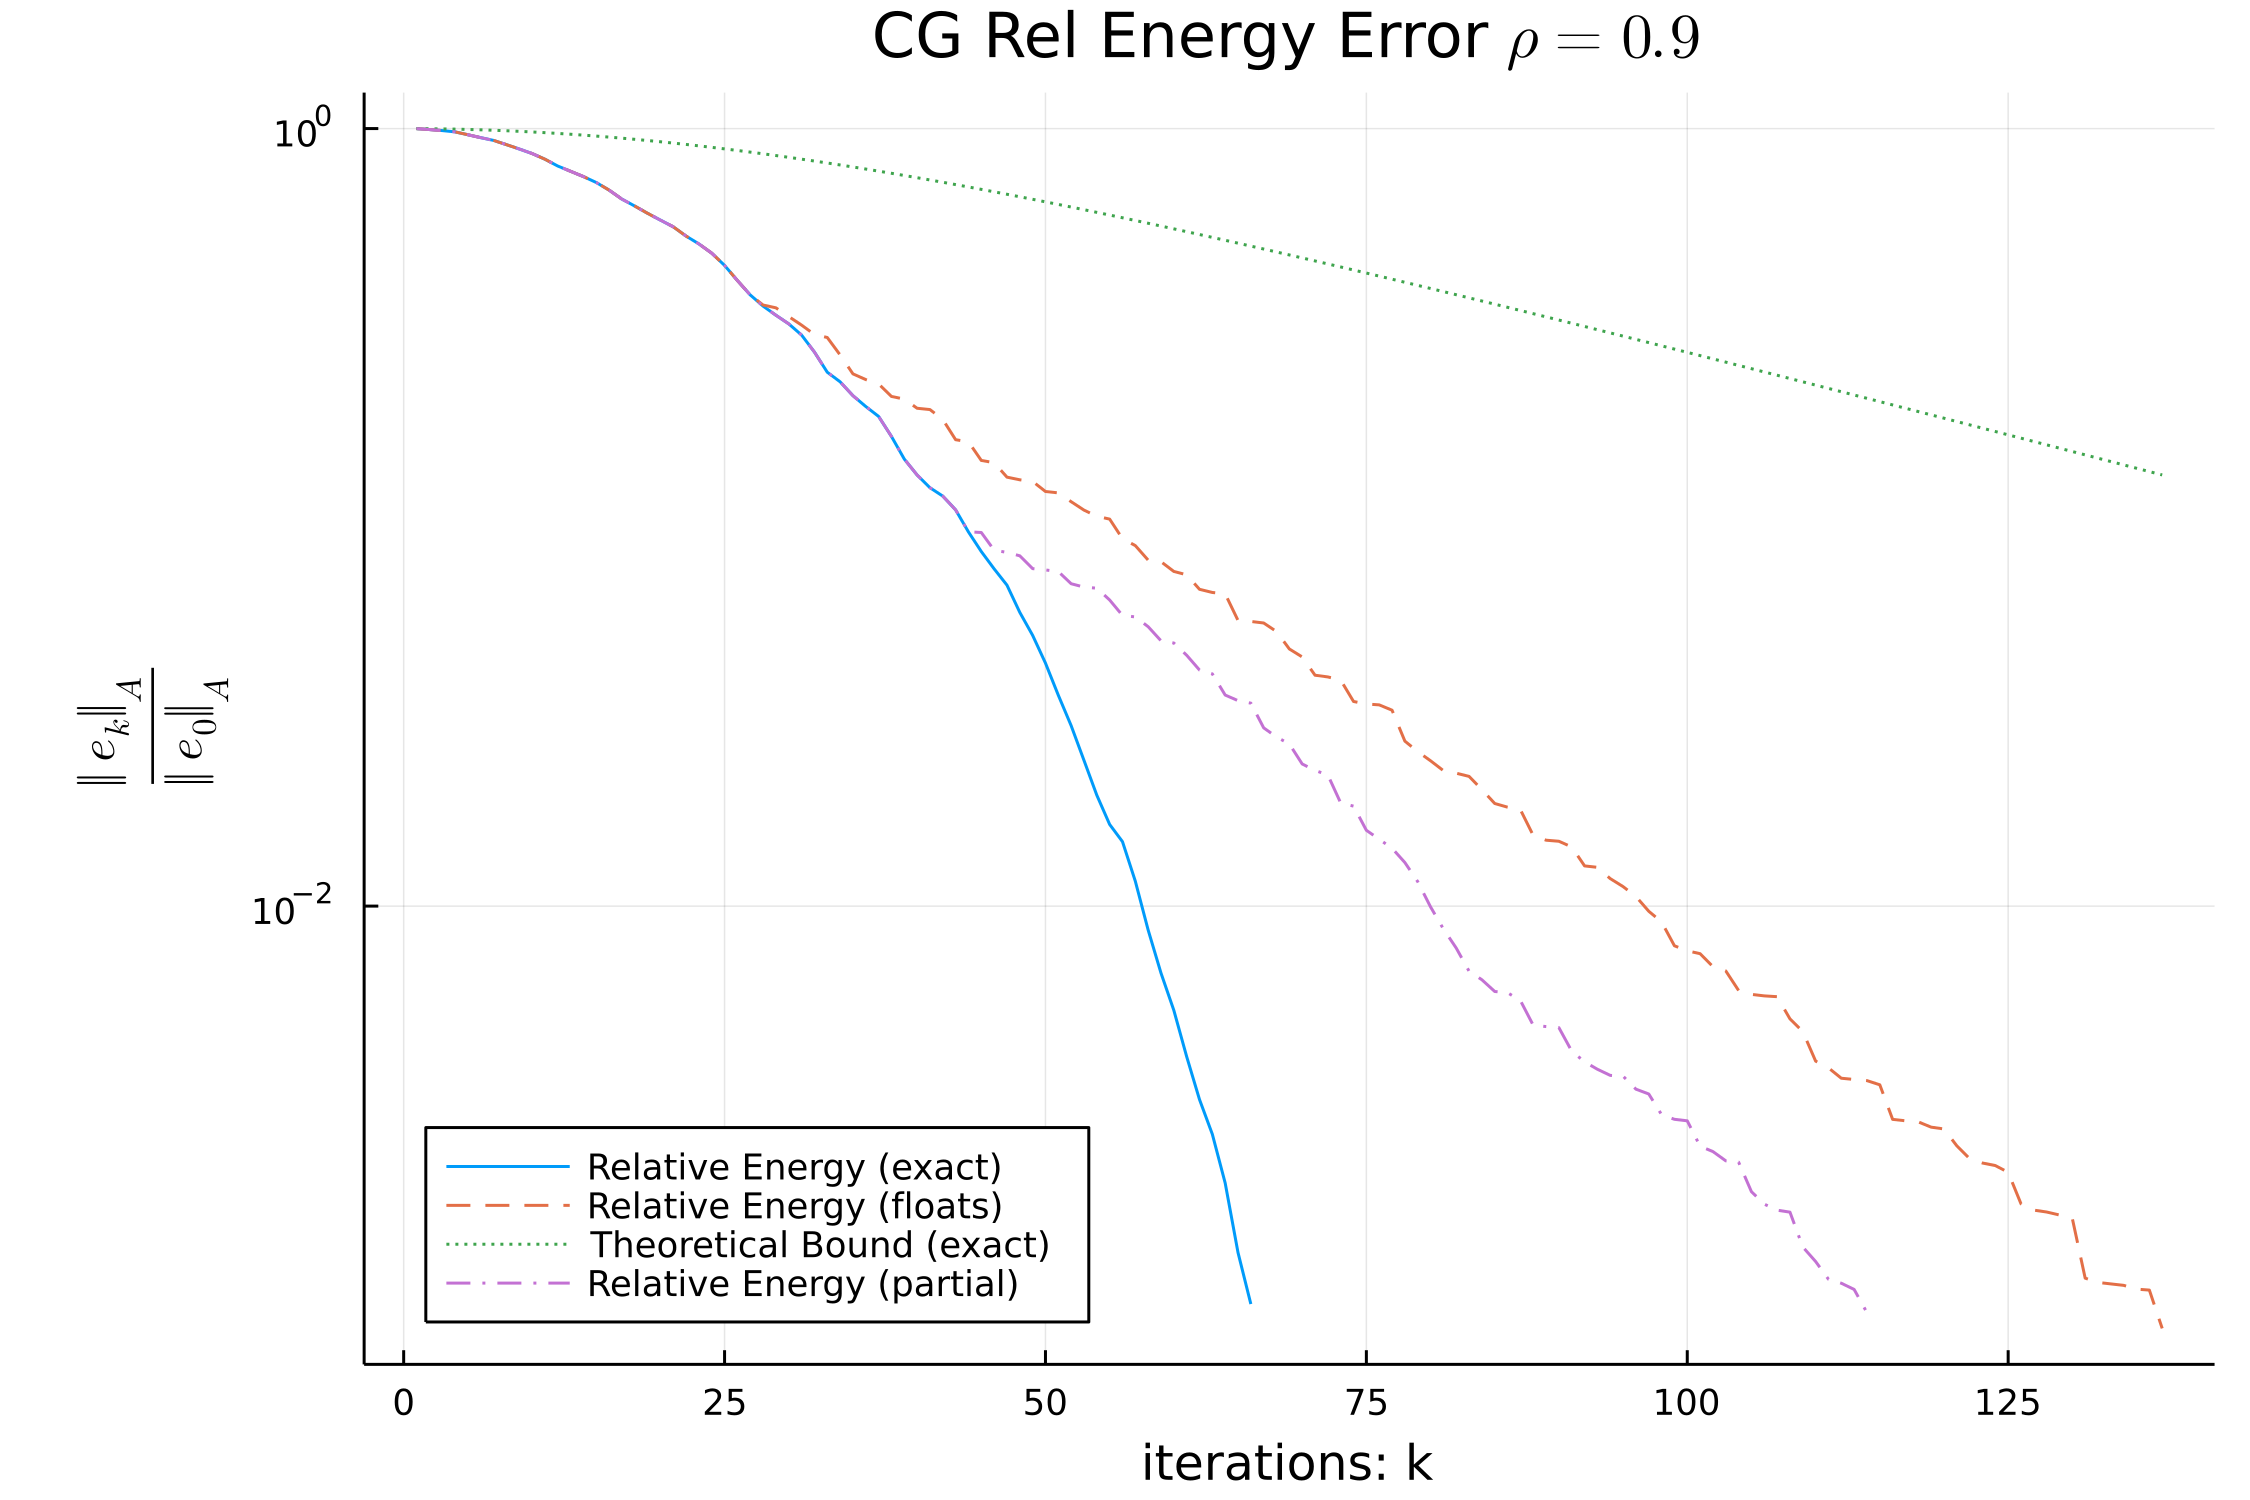
\includegraphics[width=8cm]{cg_convergence_0.9.png}
            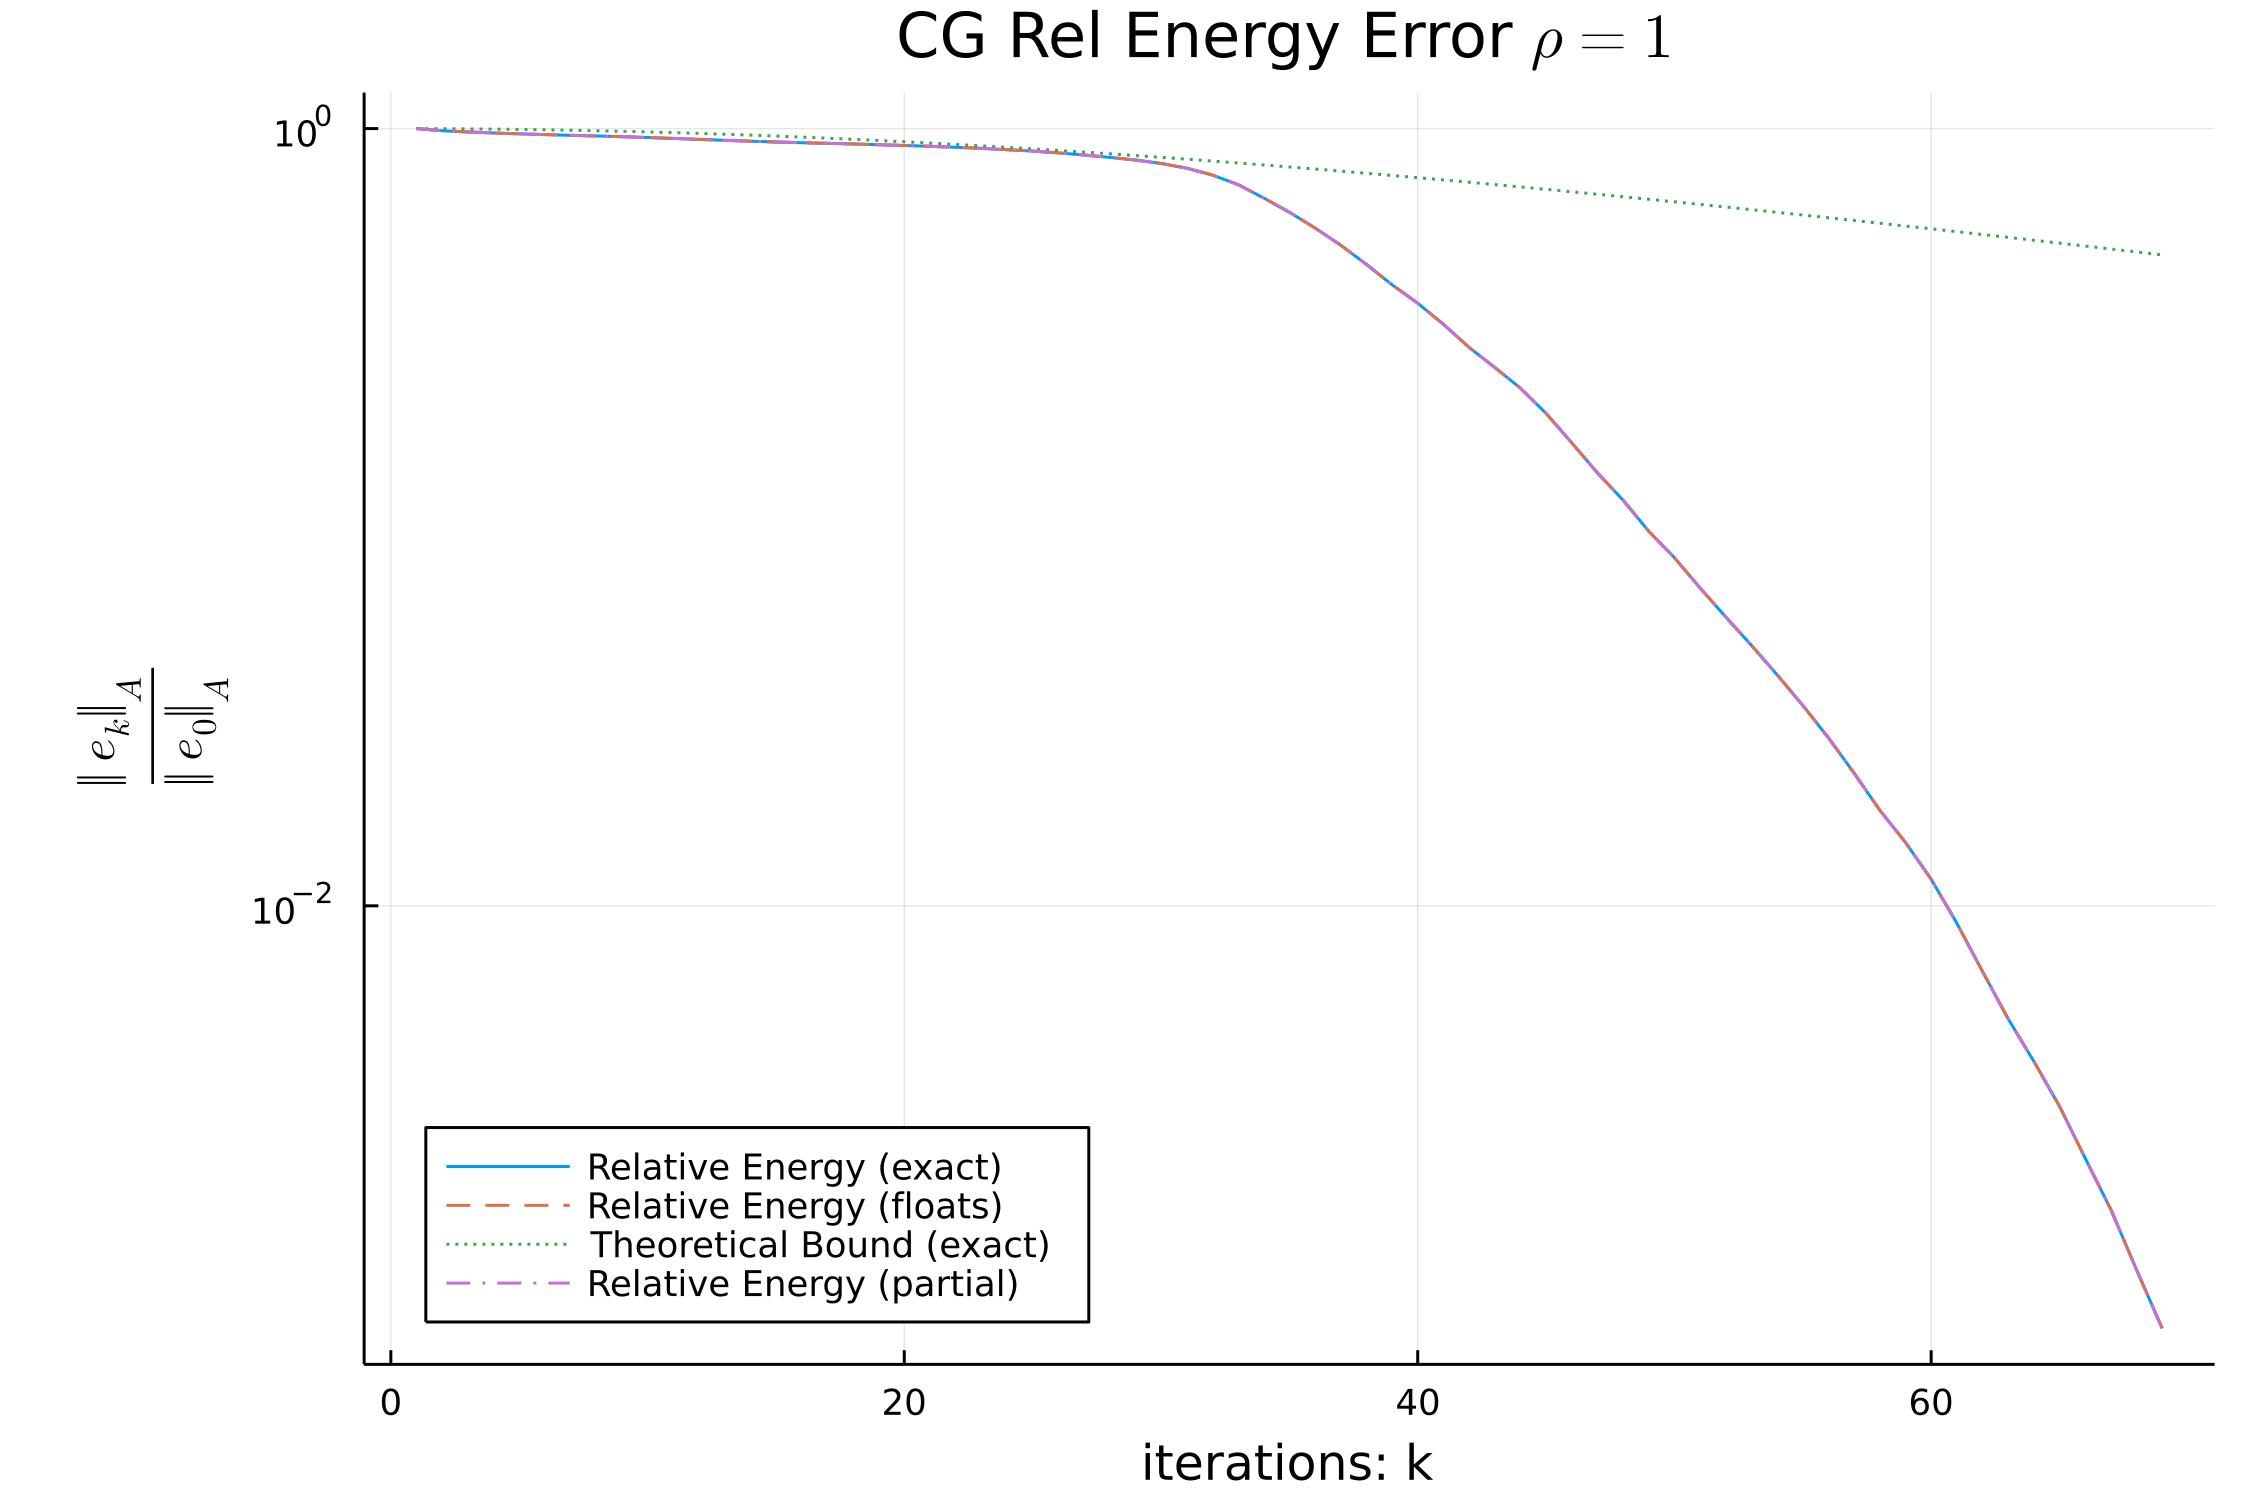
\includegraphics[width=8cm]{cg_convergence_1.png}
            \caption{
                The relative energy norm error for different methods. Blue solid line: The exact conjugate gradient convergence. Purple dot dashed: The conjugate gradient that is partially orthogonalized with previous 8 residual and conjugate vectors. orange dashed: the Original conjugate gradient. Green dot: The tighter theoretical upper bound derived by Chebyshev (\hyperref[line:CG_Cheb_Bound]{\ref*{line:CG_Cheb_Bound}}). Left: $\rho = 0.9$; right: $\rho = 1$, the matrix is $64\times 64$
            }
        \end{figure}\label{fig:1}
        The Chebyshev bound is no longer a tight bound because the distribution of the eigenvalues is not perfectly uniform. The partially orthogonalized methods diverge from the exact error after more steps of iterations compared to the relative error without any orthogonalizations. These are seen in \hyperref[fig:1]{(fig \ref*{fig:1} left)}. In contrast, on the right, then the eigenvalues are uniformly distributed, the convergence of all 3 types of methods aligns with the exact convergence in \hyperref[fig:1]{(fig \ref*{fig:1} right)}. 
        \begin{remark}
            The convergence is disappointing under floating-point arithmetic and the promised efficiency of the algorithm is not there anymore if the matrix is not necessarily ill-conditioned. Just from \hyperref[fig:1]{(fig \ref*{fig:1})} it seems like outlier eigenvalues provide fast convergence under full orthogonalization, but not for floating point. 
        \end{remark}
    \subsection{Paige's Convergence rate of CG under Floating Points}
        In this section we present the backwards analysis of the CG convergence rate in a more thorough manner and examine its consequences. When floating-point arithmetic is used, the eigenvalues of the tridiagonal matrices might introduce ghost eigenvectors for the Lanczos Iterations, and using the equivalence of the Lanczos iterations and CG, we can capture a posteriori bound on how much the error is exactly during the iterations of CG. 
        \subsubsection{Bounding the Relative Residuals}
            Recall from proposition \hyperref[prop:Lanczos_Vectors_and_Residuals]{Proposition \ref*{prop:Lanczos_Vectors_and_Residuals}} that the residual of the CG can be expressed in terms of the Lanczos vectors. However, the Lanczos iterations under floating doesn't produces perfectly orthogonal Lanczos Vectors (The lost of orthogonality is experimented and visualized in the next section), $\tilde{Q}_k$ is not quiet orthogonal, which would also means that $\tilde{Q}_k^HA\tilde{Q}_k\approx T_k$ where $T_k$ is the results from the Lanczos iterations will not equal to $\tilde{Q}^T_KA\tilde{Q}_k$. However the Lanczos iterations will still solve for $y_k$ using the expression $y_k = \beta T^{-1}_k\xi_1$, the algorithm still thought $T_k$ produced by itself is perfectly tridiagonal. As a result, the algorithm never quite finds the optimal under the conjugate basis. At first glance, tiny round-off errors in the Lanczos vectors are very problematic. 
            \par
            Surprisingly, the recurrence formula for Lanczos still holds to some extent, in addition we can leverage the fact that $y_k$ is solved exactly and assume: $y_k = \beta T^{-1}\xi_1$ is at least, exact. Then it left us with fewer types of floating-point errors to keep track of. Next, we proceed to look for the residual of the CG algorithm by assuming that the Lanczos recurrences: 
            \begin{align}
                AQ_k = Q_{k + 1} \begin{bmatrix}
                    T_k
                    \\
                    \beta_k \xi_k^T
                \end{bmatrix} + F_k
            \end{align}
            Reader, please reflect on the fact that the $Q_k$ which is not orthogonal, and we are fixing the recurrences with $F_k$, a matrix representing the floating error to correct it so that the equality holds true. $\Vert F_k\Vert$ is small and it's on the magnitude of machine epsilon. 
            \begin{align}
                r_k &= r_0 - AQ_ky_k
                \\
                r_k &= r_0 - 
                    \left(
                        Q_{k + 1} \begin{bmatrix}
                            T_k
                            \\
                            \beta_k \xi_k^T
                        \end{bmatrix}
                        + 
                        F_k
                    \right)
                y_k
                \\
                r_k &= 
                \underbrace{\left(
                    r_0 - Q_{k + 1}\begin{bmatrix}
                        T_k
                        \\
                        \beta_k \xi_k^T
                    \end{bmatrix}y_k
                \right)}_{= -\beta_k\xi_k^Ty_kq_{k + 1}} + F_k \beta T_k^{-1}\xi_1
                \\
                \implies
                \frac{\Vert r_{k + 1}\Vert}
                {
                    \Vert r_0\Vert
                } &\le
                \beta_k \Vert
                    \xi_k^T T_k^{-1}\xi_1 q_{k + 1}
                \Vert + 
                \Vert F_kT_k^{-1}\xi_1 \Vert
                \\
                \frac{\Vert r_{k + 1}\Vert}
                {
                    \Vert r_0\Vert
                } 
                &\le 
                \beta_k |
                    \xi_k^T T_k^{-1}\xi_1
                | + 
                \Vert F_k\Vert  \Vert T_k^{-1}\xi_1\Vert
            \end{align}
            We make use of \hyperref[prop:Lanczos_Vectors_and_Residuals]{Proposition \ref*{prop:Lanczos_Vectors_and_Residuals}} and obtain a similar expression because it didn't make use of the fact that $Q_k$ is orthogonal. This time, we take $F_k$ into account. The residual is now bounded by the sum of scalar $\xi_k^T T_k^{-1}\xi_1$ and the floating-point error matrix $F_k$ produced by the Lanczos iterations. 
            \begin{remark}[Running Lanczos on Tridiagonal with $q_1=\xi_1$]\label{remark:CG_Float_Remark}
                We can bound the first term that made up the upper bound for the residual of CG using previous convergence results of CG under exact arithmetic; recall \hyperref[theorem:CG_Convergence_Rate]{CG convergence rate (theorem \ref*{theorem:CG_Convergence_Rate})}. It can be applied here for the first term in (5.3.6): 
                $\beta_k |
                \xi_k^T T_k^{-1}\xi_1|$. 
                \par
                This is true because if we were to perform an CG on the $T_{k + 1}$ produced by the finite precision algorithm with the initial Lanczos vector $q_1$ being $\xi_1^{(n)}$, then its residual $\overline{r}_{k}$ would be exact and it's given as $-\beta_kT_{k}^{-1}\xi_kq_{k + 1}$, but with $q_{k + 1} = \xi_{k + 1}^{(n)}$, the $k + 1$ th standard basis vector in $\mathbb R^{n}$, and $T_k = (T_{k + 1})_{1:k, 1:k}$ . And to our excitement, we already have the bound for $\overline{r}_{k+1}$ proven in \hyperref[theorem:CG_Convergence_Rate]{theorem \ref*{theorem:CG_Convergence_Rate}}.
            \end{remark}

        \subsubsection{Paige's Theorem and Floating-point Convergence of CG}
            We now introduce a new theorem proposed by Paige in chapter 4 of Greenbaum's book\cite{book:greenbaum}, originally appeard in C.C Paige Thesis(\textbf{CITATION NEEDED}). It gives a bound to the floating-point errors for the CG by bounding the condition number of $T_k$ from Lanczos iterations. It's stated as follows: 
            \begin{theorem}[Paige's Theorem]\label{theorem:paige1}
                The eigenvalues $\theta_i^{(j)}, i = 1, \cdots, j$ of the tridiagonal matrix $T_j$ satisfies: 
                \begin{align}
                    & 
                    \lambda_1 - j^{5/2}\epsilon_2\Vert A\Vert 
                    \le \theta_i^{(j)}
                    \le 
                    \lambda_n + j^{5/2}\epsilon_2\Vert A\Vert
                    \\
                    &
                    \epsilon_2 := \sqrt{2}\max\{6\epsilon_0, \epsilon_1\}
                \end{align}
            \end{theorem}
            Along with this theorem, the following quantities from Paige are also defined and cited in Greenbaum book chapter 4. 
            \begin{align}
                & \epsilon_0 \equiv 2(n + 4)\epsilon
                \\
                & \epsilon_1 \equiv 2(7 + m \Vert  \;|A|\;\Vert/\Vert A\Vert)\epsilon
                \\
                & \epsilon_0 < \frac{1}{12} \quad k(3\epsilon_0 + \epsilon_1) < 1
                \\
                & \Vert F_k\Vert \le \sqrt{k}(\epsilon_1) \Vert A\Vert
                \\
                & \Vert q^T_jq_j -1\Vert \le 2\epsilon_0
                \\
                & \beta_j \le \Vert A\Vert(1 + (2n + 6)\epsilon + j(3\epsilon_0 + \epsilon_1))
            \end{align}
            The quantity $k$ is the current iterations number of the Lanczos Iterations, $j\le k$. $m$ is the maximum number of non-zero elements in the matrix $A$. 
            Using Paige's theorem, we can bound the condition number for the matrix $T_{k + 1}$ produced by the finite precision Lanczos, which is given by: 
            \begin{align}
                \tilde{\kappa} = \frac{\lambda_n + (k + 1)^{5/2}\epsilon_2\Vert A\Vert}
                {\lambda_1 - (k + 1)^{5/2} \epsilon_2\Vert A\Vert}
            \end{align}
            Using \hyperref[remark:CG_Float_Remark]{(remark \ref*{remark:CG_Float_Remark})}, we can make the following proposition
            \begin{prop}
                \begin{align}
                    | \beta_k\xi_k^TT_k^{-1}\xi_1 | \le 
                    2 \sqrt{\tilde{\kappa}}\left(
                        \frac{\sqrt{\tilde{\kappa}} - 1}{\sqrt{\tilde{\kappa}} + 1}
                    \right)^k
                \end{align}    
                Where $\tilde\kappa$ is the bound of the condition number of the $T_k$ matrix (from (5.3.15)), the tridiagonal matrix produced by the finite precision Lanczos. 
            \end{prop}
            \begin{proof}
                Using the \hyperref[lemma:Relative_Energy_Norm_and_Relative_2_Norm_Conversions]{lemma \ref*{lemma:Relative_Energy_Norm_and_Relative_2_Norm_Conversions} in appendix}, we can derive the relations between the 2-norm of the relative residuals and the energy norm of the relative error: 
                \begin{align}
                    \frac{\Vert Ae_k\Vert}{\Vert Ae_0\Vert}
                    & \le 
                    \kappa(T_k)\frac{\Vert e_k\Vert_A}{\Vert e_0\Vert_A}
                    \le 2\sqrt{\kappa(T_k)}
                    \left(
                        \frac{\sqrt{\tilde{\kappa}} - 1}{\sqrt{\tilde{\kappa}} + 1}
                    \right)^k
                    \\
                    \frac{\Vert r_k\Vert}{\Vert r_0\Vert} &= 
                    | \beta_k\xi_k^TT_k^{-1}\xi_1 | \quad \text{by \hyperref[remark:CG_Float_Remark]{(remark \ref*{remark:CG_Float_Remark})}}
                    \\
                    \implies | \beta_k\xi_k^TT_k^{-1}\xi_1 | 
                    &\le 
                    2 \sqrt{\tilde{\kappa}}
                    \left(
                        \frac{\sqrt{\tilde{\kappa}} - 1}{\sqrt{\tilde{\kappa}} + 1}
                    \right)^k
                \end{align}
                The third inequality is simply from \hyperref[theorem:CG_Convergence_Rate]{CG Convergence Rate (theorem \ref*{theorem:CG_Convergence_Rate})} when we assume that the eigenvalues are uniformly distributed convex hull of the spectrum of $A$. The first fraction is actually the relative error of the 2-norm of the residual because $Ae_k = r_k$ by definition. Substituting the quantity $\kappa(T_k)$, the condition number of the matrix $T_k$, which we figured out using Paige's theorem and denoted it as $\tilde{\kappa}$. 
            \end{proof}
            Finally, if we assume that $T_k^{-1}$ is actually invertible, which requires that the conditions for all the quantities: $\epsilon_0, \epsilon_1$ holds true, and $\lambda_1 - (k + 1)^{5/2} \epsilon_2\Vert A\Vert > 0$. Finally, we make can bound the relative residual of the CG algorithm by considering: 
            \begin{align}
                \frac{\Vert r_{k + 1}\Vert}
                {
                    \Vert r_0\Vert
                } &\le
                \beta_k \Vert
                    \xi_k^T T_k^{-1}\xi_1 q_{k + 1}
                \Vert + 
                \Vert F_kT_k^{-1}\xi_1 \Vert
                \\
                & \le 
                \beta_k|\xi_k^T T_k^{-1}\xi_1|
                \Vert q_{k + 1}\Vert + 
                \Vert F_k\Vert  \Vert T^{-1}_k\xi_1\Vert
                \\
                & \le 
                2 \Vert q_{k + 1}\Vert\sqrt{\tilde{\kappa}}
                    \left(
                        \frac{\sqrt{\tilde{\kappa}} - 1}{\sqrt{\tilde{\kappa}} + 1}
                    \right)^k
                + 
                \sqrt{k}(\epsilon_1) \Vert A\Vert 
                \Vert T^{-1}_k\Vert
            \end{align}
            Now, observe that $|q_j^Tq_j - 1|\le 2\epsilon_0$ from (5.3.13), which implies that $\Vert q_{k + 2}\Vert^2 \le (1 + 3\epsilon_0)$ which is $\Vert q_{k + 1}\Vert \le \sqrt{1 + 2\epsilon_0}$. In pursuit of mathematical beauty, we look for alternative expression for the quantity $\Vert A\Vert \Vert T^{-1}_k\Vert$ giving us: 
            \begin{align}
                \Vert A\Vert\Vert T_k^{-1}\Vert &= \frac{\lambda_n}{\lambda_1 - k^{5/2}\epsilon_2\Vert A\Vert} \le \tilde{\kappa}
                \\
                \implies 
                \frac{\Vert r_{k + 1}\Vert}
                {
                    \Vert r_0\Vert
                } &\le 
                2  \sqrt{1 + 2\epsilon_0}\sqrt{\tilde{\kappa}}
                    \left(
                        \frac{\sqrt{\tilde{\kappa}} - 1}{\sqrt{\tilde{\kappa}} + 1}
                    \right)^k
                + \sqrt{k}(\epsilon_1) \tilde{\kappa}
            \end{align}
            Which completes the proof for the upper bound on the convergence rate for the Conjugate Gradient Method under floating-point arithmetic. 
            \begin{remark}
                This proof showed that the $T_{k + 1}$ generated by floating point CG is nonsingular, $\beta_k \neq 0$, the restrictions for the quantities of \hyperref[theorem:paige1]{theorem \ref*{theorem:paige1}} then the CG method will continue to converge in the future iterations. So in layman's terms, it doesn't matter if the round-off error accumulated, Conjugate Gradient will converge as long as the problem is not too insane, or $A$ being too pathological to deal with. 
                \par
                Finally, I want to point out the fact that Paige's theorem (\hyperref[theorem:paige1]{theorem \ref*{theorem:paige1}}) is derived using forward error analysis on the Lanczos Iterations, which is the absolute worst case. For most cases in modern computing platforms, the summation process of vector dot products has much higher floating-accuracy compare to older computing platforms due to the use of parallelism, or floating-point specific summation instructions, which reduces the relative sizes for the summands, hence reducing the total round-off error accumulations. The bound of convergence rate we derive can be a huge over estimation. 
            \end{remark}

    \subsection{Ghost Eigenvalues and Losing Orthogonality}
        The name Ghost Eigenvalues refers to the phenomena where the Lanczos Algorithm seems to find eigenvalues that are extremely close to each other, when in fact, those extremely close eigenvalues are a single eigenvalue of the original matrix $A$'s spectrum. The name for it comes from Trefethen's Book\cite{book:trefethen}. More specifically, the eigenvalues in $T_k$ seems to cluster closely around the true eigenvalues of the original matrix $A$, especially eigenvalues in the exterior of $A$'s spectrum. We know for a fact that the tridiagonal matrix produced via Lanczos can't have any repeated eigenvalues(\textbf{NONTRIVIAL FACT}). Floating point error propagating through the Lanczos Iterations will produce this phenomena, but the converse is not necessarily true. 
        \subsubsection{Ghost Eigenvalues Experiments}
            Here, we conducted numerical experiments and carefully reproduce the phenomena for a diagonal matrix $A$ with diagonals given by the formula: 
            \begin{align}
                \lambda_i = \left(-1 + \frac{2(i - 1)}{(n - 1)}\right)^3
            \end{align}\label{eqn:the_ill_conditioned_matrix}
            where $A\in \mathbb R^{n\times n}$. This matrix is particularly good for reproducing the phenomena. For this experiment, we set $n = 64$ and we use Float64. 
            \par
            We run the Lanczos iterations with $q_1$ being the vector of all ones, we marked the smallest and largest 10 eigenvalues during the iterations and plotted their trajectories from iteration 20 to 64. The results can be seen in \hyperref[fig:2]{(figure \ref*{fig:2} left)}. On \hyperref[fig:2]{figure \ref*{fig:2} right}, we made the plot for what would happen if the Lanczos iterations are free of numerical round-off error. We didn't use exact arithmetic, instead, we simply re-orthogonalized all the Lanczos vector $q_k$ using all previously obtained Lanczos vectors to emulate the effect, which is just an Arnoldi iteration. Please bear in mind that there are eigenvalues in the middle interior part of the spectrum, they are just not plotted in the figure. 
            \begin{figure}[H]
                \centering
                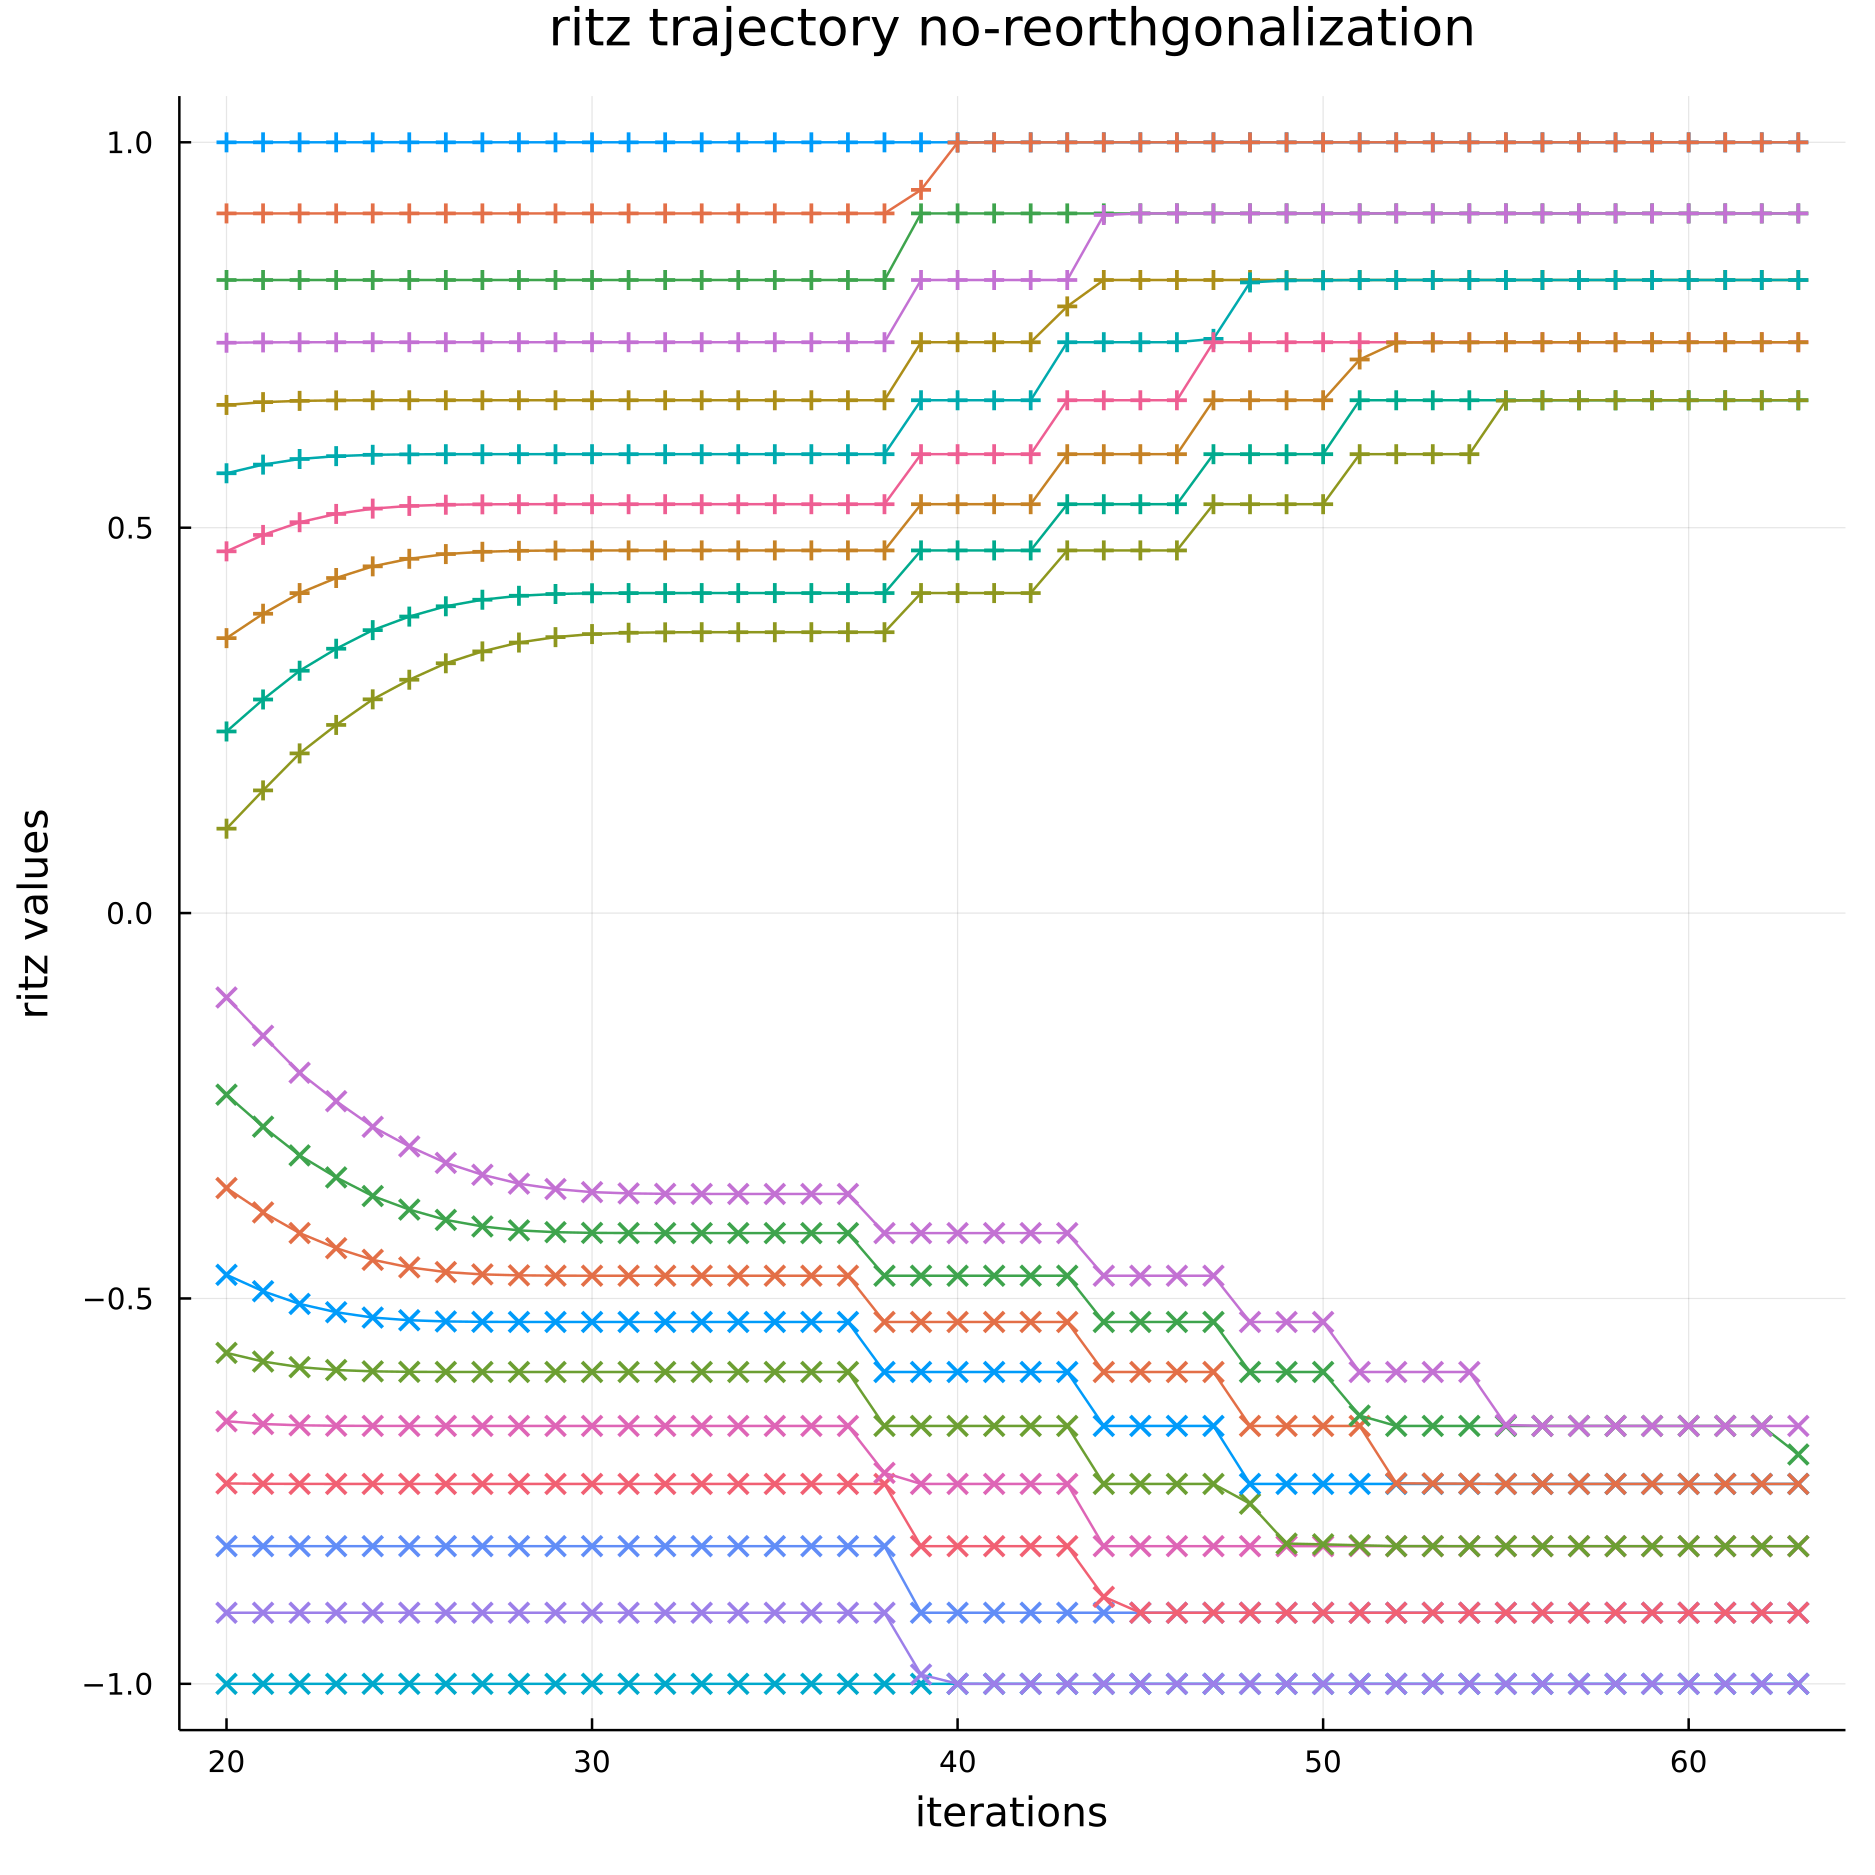
\includegraphics[width=8cm]{ritz_trajectory_plot_floats.png}
                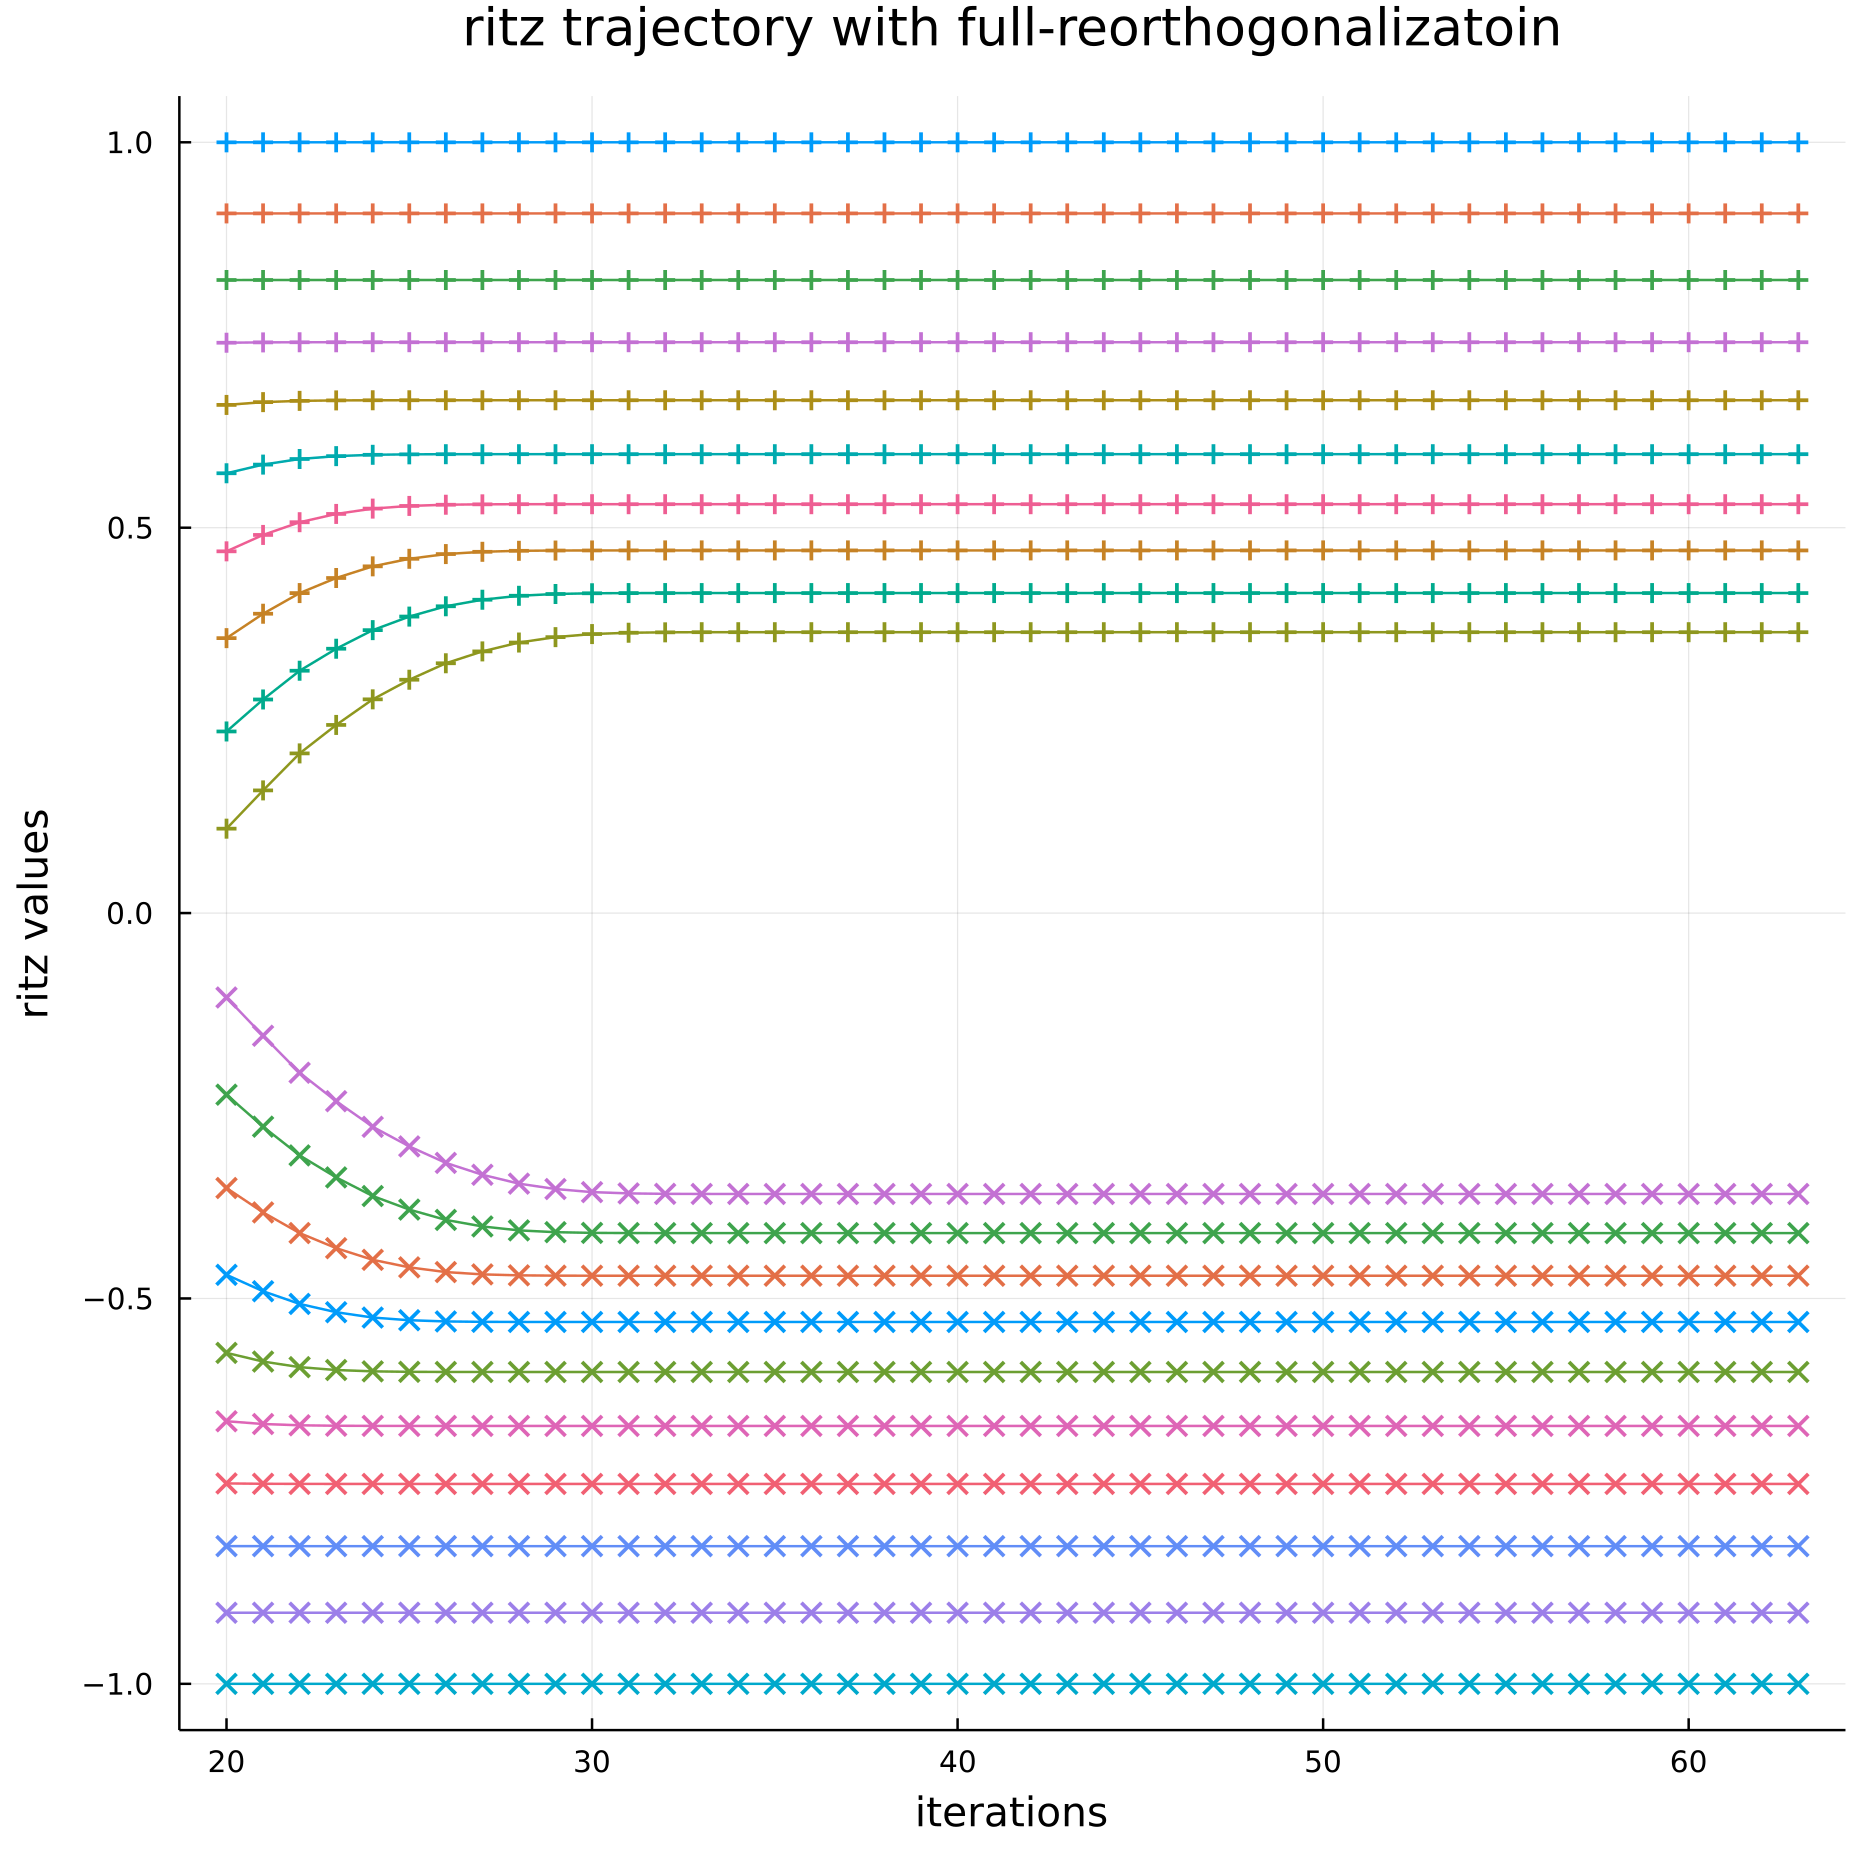
\includegraphics[width=8cm]{ritz_trajectory_plot_exact.png}
                \caption{The highest and lowest 10 eigenvalues of the matrix $T_k$ during the Lanczos Iterations are being tracked by their relative order. During each iteration, the first, the second, the third, ... etc eigenvalues of $T_k$ are linked together by a line in a different color. Left is Lanczos with numerical round-off error, right is Lanczos iterations that fully re-orthogonalize $q_k$ for each iteration which emulates the behaviors under exact arithmetic. }
            \end{figure}\label{fig:2}
            Recall from the Cauchy Interlace Theorem, the eigenvalues of the tridiagonal matrix $T_{k + 1}$ has to be in between each eigenvalues of $T_{k}$ except for the first and the last eigenvalue of $T_{k + 1}$.  This implies that, the $\theta_i^{(k)}$, the $i$ th eigenvalues during the $k$ th iteration will move monotonically upwards or downwards during the Lanczos iterations. The ghost eigenvalues on the figure appear when some of the interior eigenvalues suddenly switch to another eigenvalue's trajectory that is on the exterior of the spectrum. It appears as though the matrix $T_k$ has repeated eigenvalues, but in fact, they are not, they are just very close. 
            \par
            However, judging the eigenvalues of the matrix $T_k$ alone WILL NOT distinguish between two very close eigenvalues correspond to two different eigenvalues of $A$ or it's due to the floating-point round-off error. It also will NOT tell whether the Lanczos vectors are losing orthogonality, even if the eigenvalue trajectories seem to suggest it. We can't tell it because if I keep the matrix $T_k$ generated from a Lanczos iterations with huge amount of round-off error and all it $A$, which has eigenvalues that are extremely close to each other and their path shifts over each other on the trajectory like in \hyperref[fig:2]{fig \ref*{fig:2}}. Now consider performing another Lanczos iterations $A:=T_k$ it but with the initial vector $\xi_1$, then we will exactly reproduce $A$ itself because it's tridiagonal. But in this case, the eigenvalues of $T_k$ are exact after termination of Lanczos iteration. In this case, all eigenvalues are actually presented in the original matrix $A$, which is just $T_k$, itself. 
            \par
            In fact, the ghost eigenvalues here are produced by floating-point errors because firstly we know what the actual eigenvalues of $A$ is, we made $A$. To make sense of it better intuitively, we observe from the experiments that the loss of orthogonality of $Q_k$ happens together with ghost eigenvalues on the spectrum of $T_k$. If the $Q_k$ matrix is perfectly orthogonal, then there are no ghost eigenvalues, regardless of what the trajectories of the eigenvalues of $T_k$ look like. In fact, a corresponding plot of $Q_k^HQ_k$ are plotted in \hyperref[fig:3]{(fig \ref*{fig:3} left)} for demonstrating the loss of orthogonality for the same diagonal matrix $A$ proposed earlier. We plotted the heat map of the matrix $Q^H_kQ_k$ directly as well.
            \begin{figure}[H]
                \centering
                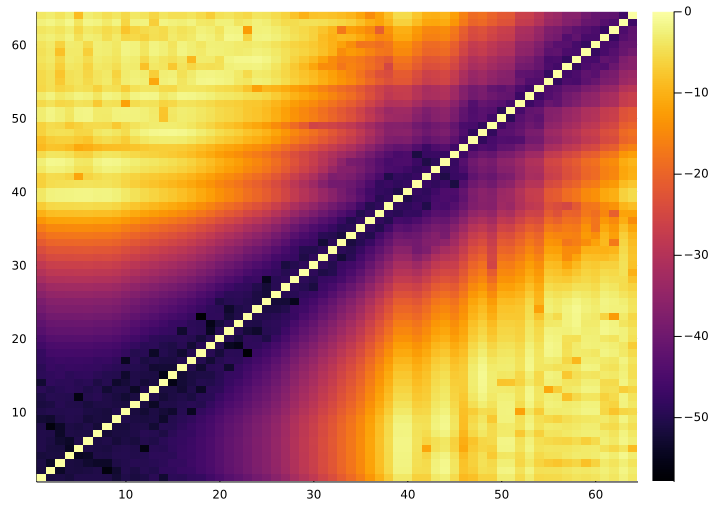
\includegraphics[width=8cm]{fig3.png}
                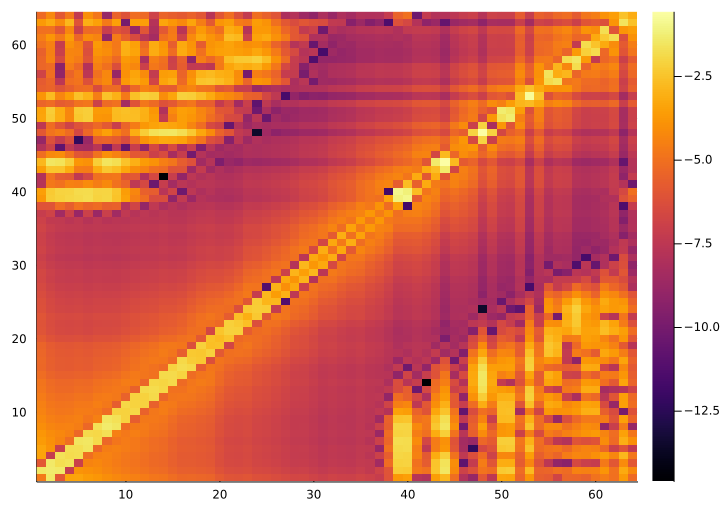
\includegraphics[width=8cm]{fig4.png}
                \caption{left: The heatmap of the plot of log2 of the absolute values of the matrix $Q^T_kQ_k$. right: The plot of $Q_k^TAQ_k$ from floating-point Lanczos iterations}
            \end{figure}\label{fig:3}
            In addition to the lost orthogonality of the matrix $Q_k$, we also visualized the actual tridiagonal matrix reproduced by $Q_kAQ_k$ which is plotted in \hyperref[fig:3]{(fig \ref*{fig:3} right)}. Observe that most of the off tridiagonal entries are non-zero and relatively huge, which doesn't worry us too much because $A$ itself has a large condition number. What is important is the blob of non-zero entries on the top left and the bottom right of the plot. And this is a hint that the loss of orthogonality will create extra errors on the off-tridiagonal parts of the matrix $T_k$. 
            \begin{remark}
                As a final remark for these numerical experiments, I suggest an intuitive way of understanding them. Which will be useful when we actually wish to analyze it rigorously. Simply put, the Lanczos Iterations might ``forget'' about the eigenvalues when it converged (Manifested as the usually stable trajectories of eigenvalues on the exterior of the spectrum for the matrix $T_k$ in \hyperref[fig:2]{(fig \ref*{fig:2})}), and when it happens, the Lanczos vectors produced by the algorithm has lost its orthogonality correspondingly, which then causes the interior eigenvalues of $T_k$ to shift, creating ghost eigenvalues that doesn't exist in the spectrum of $A$. 
                \par
                Secondly, there is another phenomenon of Ritz values during the iterations of Lanczos iterations called misconvergence. It describes the process which a Ritz value is stuck between two eigenvalues of $A$, stagnated for few iterations and then suddenly shifts away, which is extremely similar to the shifting we observed in \hyperref[fig:2]{figure \ref*{fig:2}}. It happens when 2 eigenvalues of matrix $A$ is extremely close to each other. It should not be confused with ghost eigenvalues because they are two distinct phenomena where misconvergence can happen under exact arithmetic. For more description of such phenomena, refer to the book by M. G. Cox and S. Hammarling (\textbf{CITATION NEEDED}). 
            \end{remark}
        \subsubsection{Losing Orthogonality on Ritz Vectors}
            To gain a better understanding, let's define the notion of Ritz values and Ritz vectors. For our discussion, the Ritz value $\theta_i^{(k)}$ are the $i$ th eigenvalues of the matrix $T_k$ from the and the Ritz vectors are $Q_ks_{i}^{(k)}$ where $s$ is the $i$ th eigenvector for the matrix $T_k$. Recall from \hyperref[remark:Minimal_Polynomial_from_Lanczos_Iterations]{remark 3.4.2}, the characteristic polynomial of $T_k$ is the monic polynomial that minimizes the 2-norm error for the vector $p_k(A)q_1$; intuitively, the Ritz values and Ritz vectors approximates eigenvalues and eigenvectors of matrix $A$ due to the apprixmating characteristic polynomial. Let's suppose that $s_i^{(k)}$ for $T_k$ is a good approximation for $\lambda_j$, let's consider the Lanczos iterations recurrences: 
            \begin{align}
                AQ_k &= Q_k T_k + q_{k + 1}\beta_k\xi_k^T
                \\
                AQ_ks_i^{(k)} &= \theta_j^{(k)} Q_k s_i^{(k)} + q_{k + 1}\beta_k \xi_k^Tv
                \\
                AQ_ks_i^{(k)} &= \theta_j^{(k)} Q_k s_i^{(k)} + \beta_kq_{k + 1}(s_i^{(k)})_k
                \\
                AQ_ks_i^{(k)} - \theta_j^{(k)} Q_k s_i^{(k)} &=   \beta_kq_{k + 1}(s_i^{(k)})_k
            \end{align}
            Upon brief examinations, convergence of the Ritz value $\theta_{i}^{(k)}$ depends on $\beta_k$ and $(s_i^{(k)})_k$, intuitively as the Krylov subspace expands, it contains more and more space for the the eigenvectors of $A$, and the Ritz vector will have more ``room'' to get closer to the eigenvector of $A$, by the approximation property of Lanczos. Assuming good convergence of $s_i^{(k)}$ convergences so that the value of $\beta_k, (s_i^{(k)})_k$ are both small (it's true regardless of orthogonality of $Q_k$), then we consider the projection of most recent lanczos vector $q_k$ onto the Ritz vector $Q_ks_i^{(k)}$, which is $q_k^TQ_ks_i^{(k)} = (s_i^{(k)})_k$. We expect the projection onto the Ritz vector to be small if the Ritz vector is converging to an eigenvector of $A$.  
            \par
            However, under floating-point arithmetic, once the Ritz vector $s_i^{(k)}$ is converging to an eigebvalue of $A$, then the projection of the latest Lanczos vector onto the Ritz vector begins to grow. On the plot showed in \hyperref[fig:4]{figure \ref*{fig:4}}, we projected the log absolute value of $q_k^TQ_ks_i^{(k)}$ for $i=1, 2, 3$ for all $k=20, \cdots, 64$, and we used the same setup from the last section where we demonstrated ghost eigenvalues. For comparison, \hyperref[fig:5]{figure \ref*{fig:5}} showed us what happens in exact arithmetic. One very important observation to make from \hyperref[fig:5]{figure \ref*{fig:5}} is that the peak of the blue curve, projection onto the largest Ritz value happens around iteration 3.8, and around that exact same iteration in \hyperref[fig:2]{figure \ref*{fig:2}} is when the second-largest eigenvalue of $T_k$ decides to shift over to the blue curve. Bear in mind that this is in a log plot, and without the log it looks like a sharp spike. 
            \par
            While floating arithematic may sometimes cause the most recent Lanczos vector to lose orthogoality against converged Ritz vectors, the converse is not true. The phenomena itself doesn't imply the fact that floating point error is present and it's causing lost of orthogonality of Lanczos iterations, much similar to what had been discussed about ghost eigenvalues. To illustrate, an experiment is conducted in this way: 
            \begin{enumerate}
                \item [1.] $T_n$ is generated from the diagonal matrix $A$ from finite precision Lanczos iterations. The same setup from \hyperref[eqn:the_ill_conditioned_matrix]{ghost eigenvalues \ref*{eqn:the_ill_conditioned_matrix}}. 
                \item [2.] Lanczos is then performed on $T_k$ initalized with $q_1 = \xi_i$. 
                \item [3.] The projection the most recent lanczos vector $q_k$ is projected onto $Q_ks_i^{(k)}$ for $1\le i \le 3$. Notice that $Q_k$ is gonna be the $k\times k$ identity matrix. 
            \end{enumerate}
            The results of the projection is showed in \hyperref[fig:6]{fig \ref*{fig:6}}. Please observe that prjection onto the second Ritzvector $Q_ks_2^{(k)}$ seems to decrease and them jumped up again. This happens around the same iterations when the second largest eigenvalue of $T_k$ shift to the trajectory of the largest eigenvalue in \hyperref[fig:2]{fig \ref*{fig:2} left}. 
            \begin{figure}[H]
                \centering
                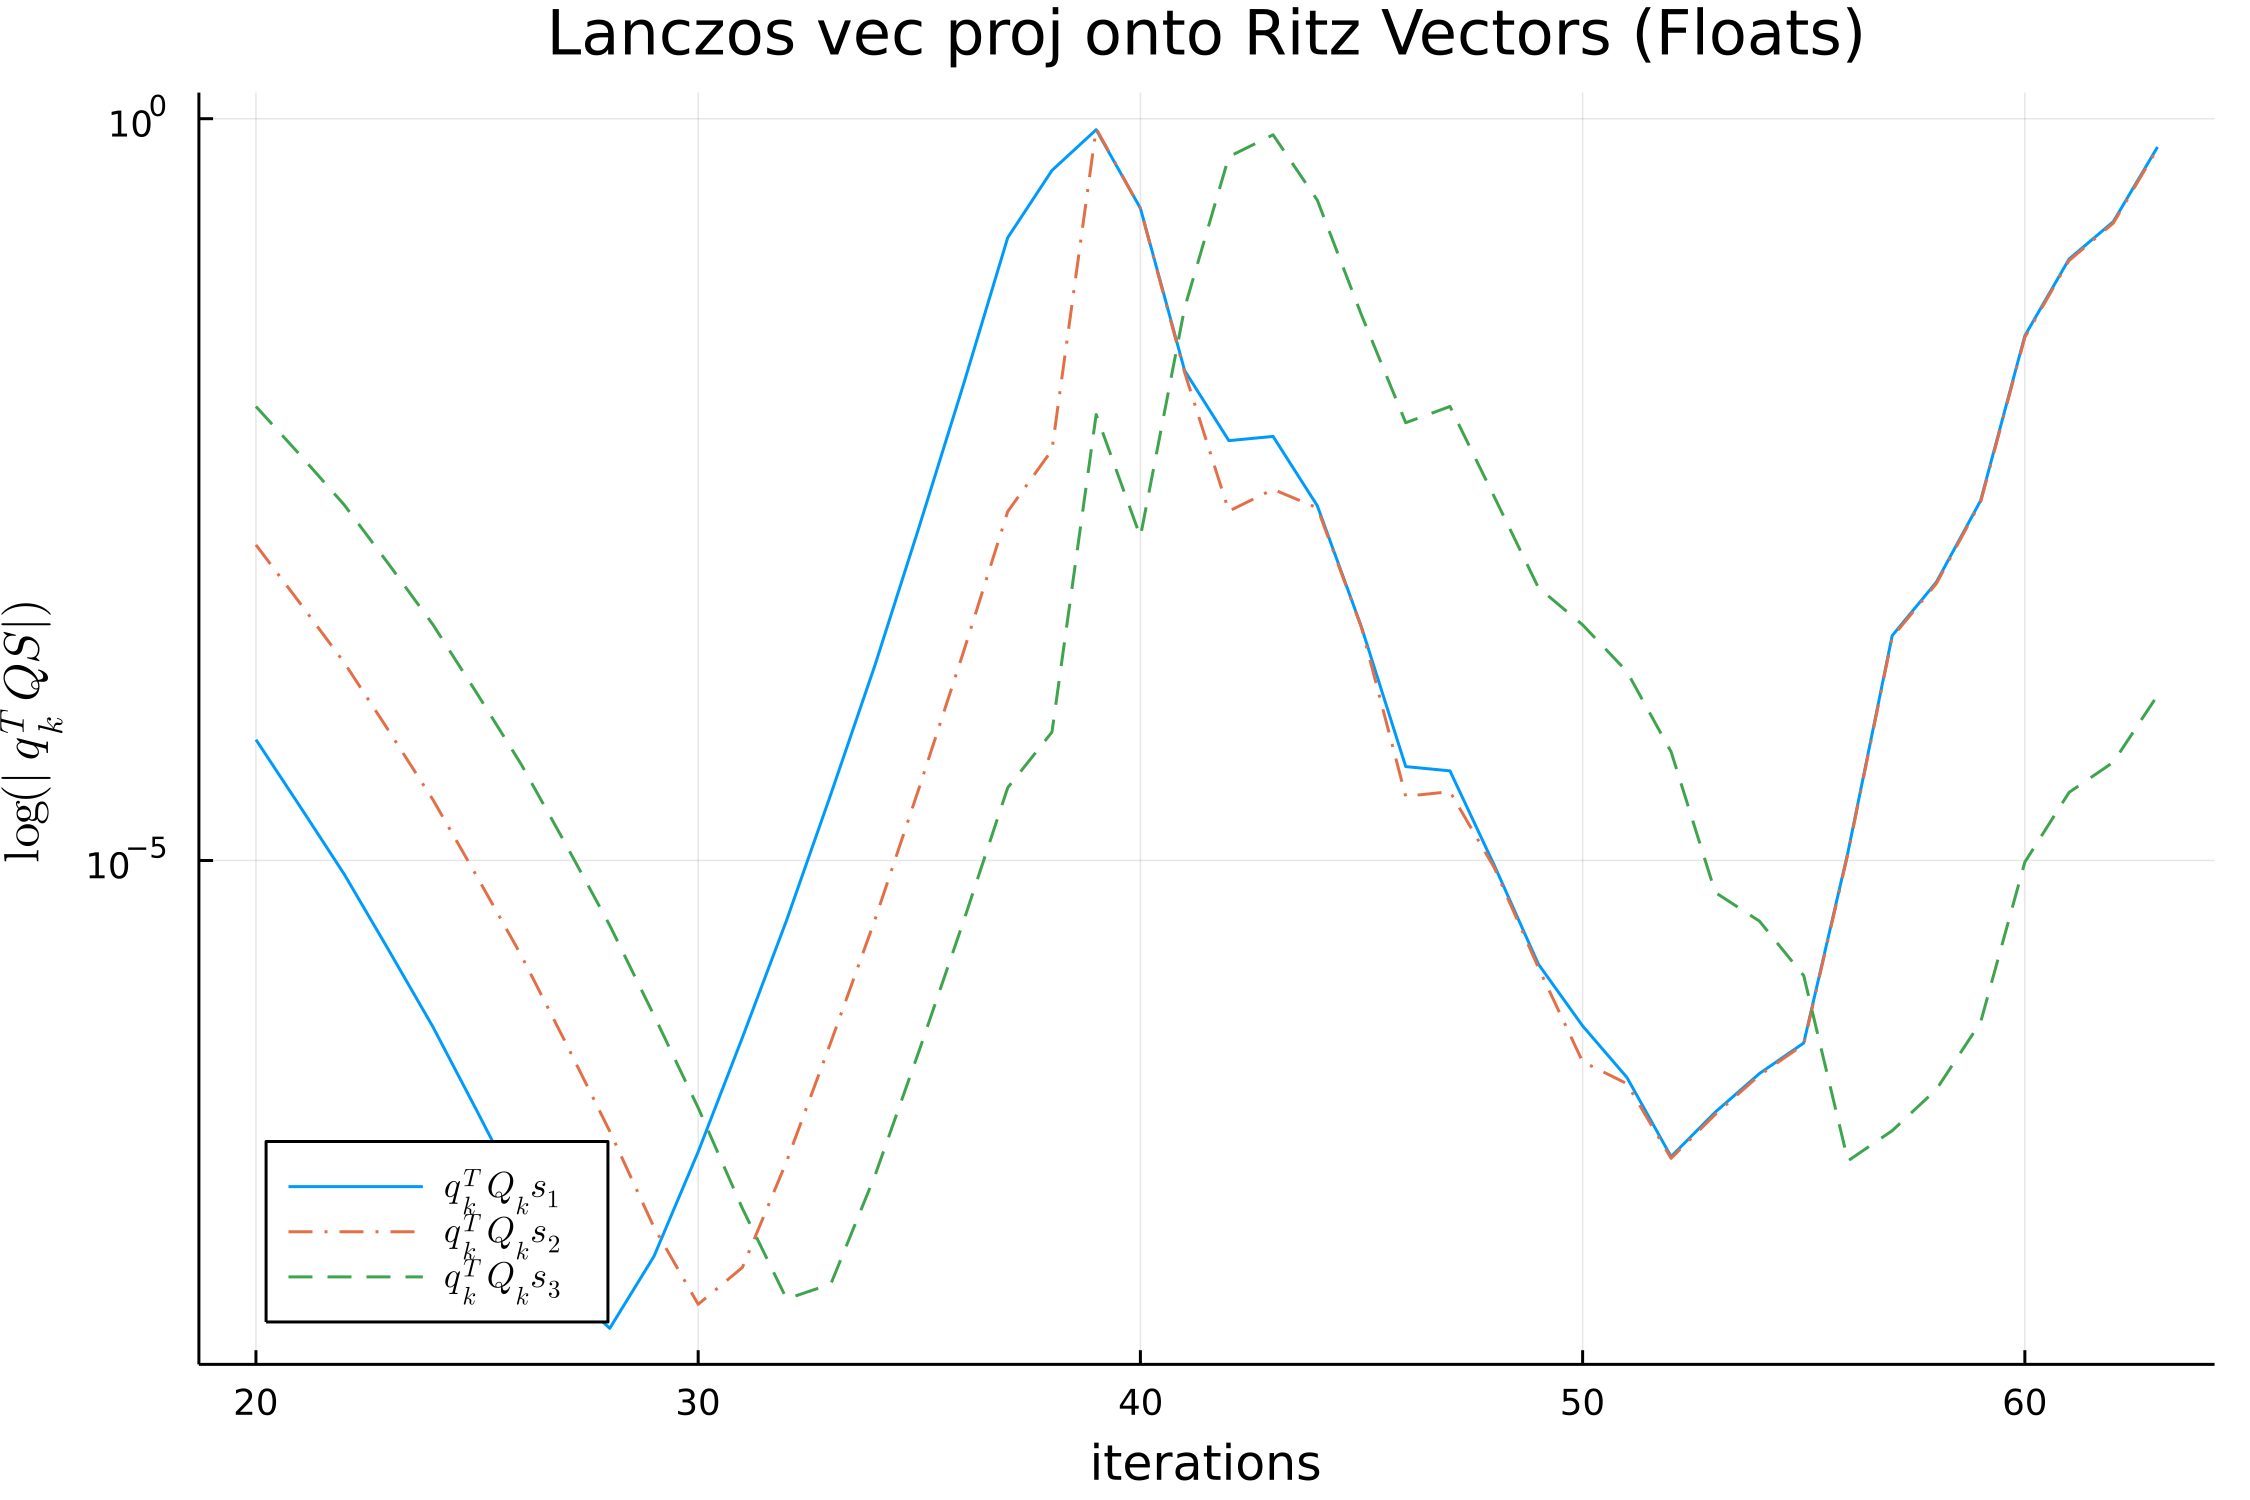
\includegraphics[width=14cm]{lanczos_proj_on_ritz_float.png}
                \caption{Projection of floating-point Lanczos vector $q_k$ onto 3 of the largest Ritz vectors: $Q_ks_i^{(k)}$, for $i = k, k - 1, k - 2$
                }
            \end{figure}\label{fig:4}
            \begin{figure}[H]
                \centering
                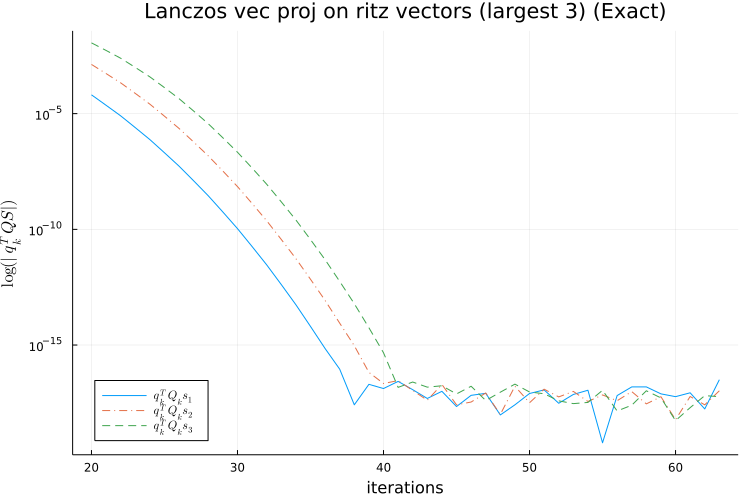
\includegraphics[width=14cm]{lanczos_proj_on_ritz_exact.png}
                \caption{prHjection of the exact Lanczos vector $q_k$ onto 3 of the largest Ritz vectors: $Q_ks_i^{(k)}$, for $i = k, k - 1, k - 2$}
            \end{figure}\label{fig:5}
            \begin{figure}[H]
                \centering 
                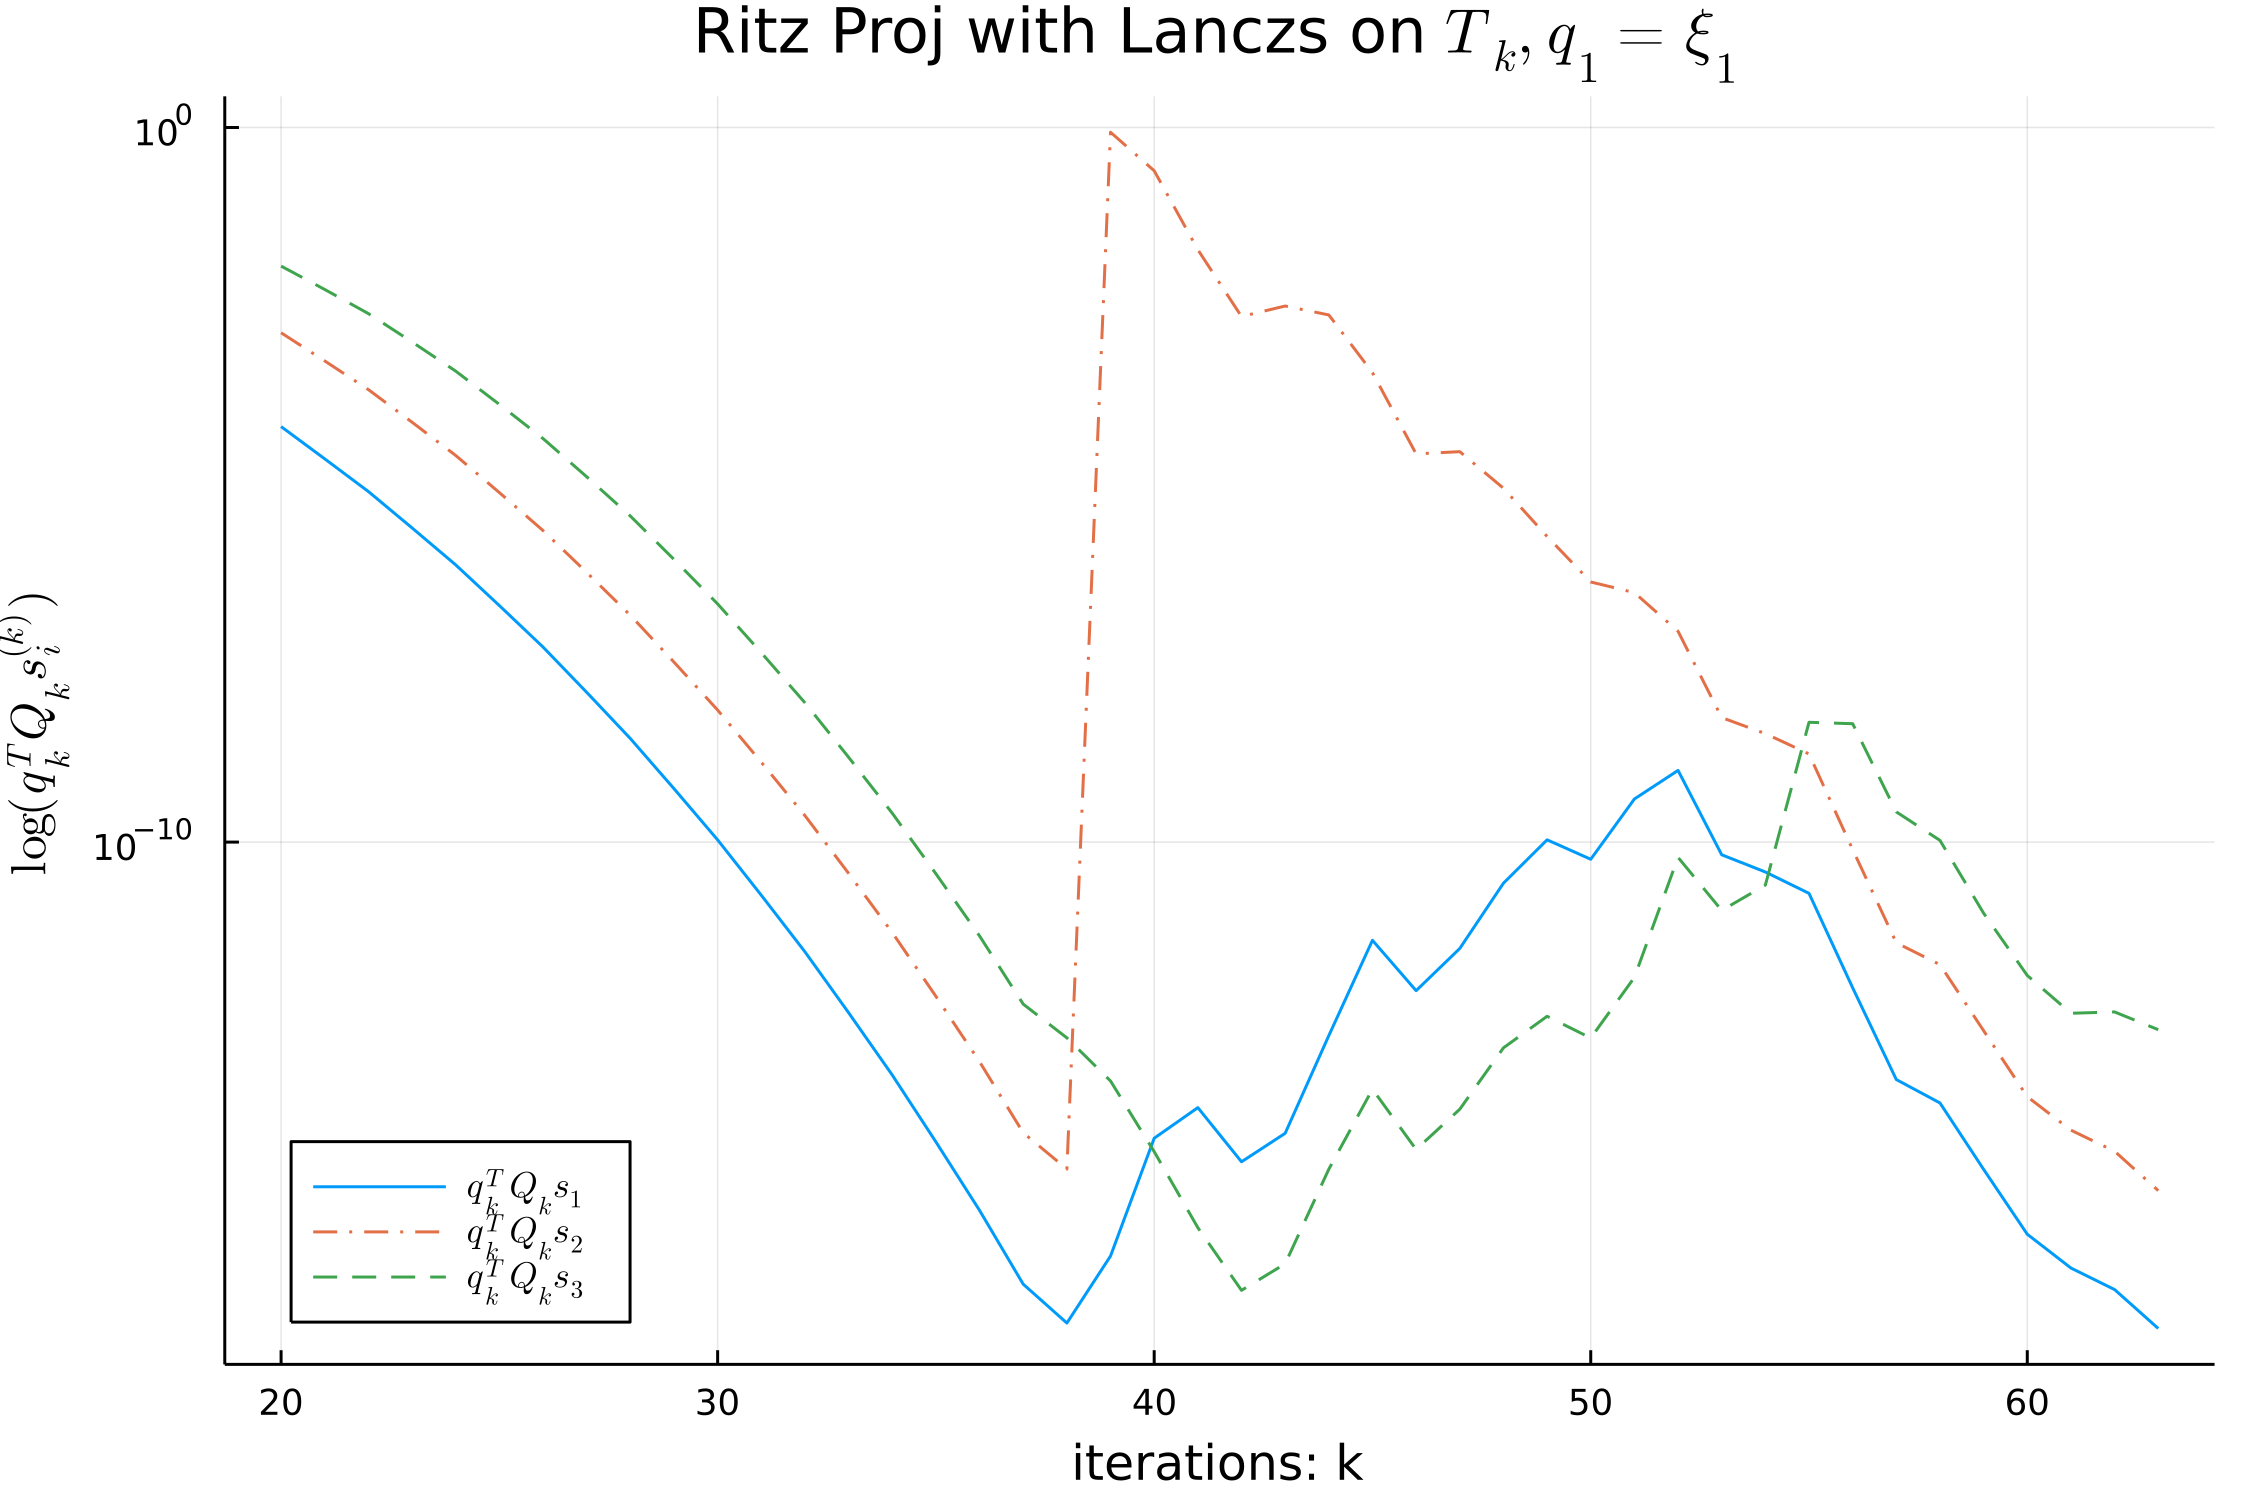
\includegraphics[width=14cm]{ritz_proj_tridiagonal.png}
            \end{figure}\label{fig:6}
            \begin{remark}[Convergence Bounds on Ritzvalues]
                The above presentation for the convergence of a Ritz Value and Ritz vector is an oversimplification. What happened is complicated. Firstly, $\beta_k$ from the tridiagonal matrix is positive because it's the norm of the characteristic polynomial of $T$ under some weighted measured (\textbf{PROOFS MISSING}), so it's positive. It empirally tends to decrease but it's just an empiracal rule, and this would implies that to prove the convergecne one would need to look into the quantity $(s_i^{(k)})_k$ as well. 
                \par
                It's not always the case that $\theta_1^{(j)}$ for example, it's the best approximation for $\lambda_1$ of $A$, and it's especially true when iterations $j$ is relative small compare to $n$. The theoretical importance is to find an interval of how far are the $\lambda_i$ from $\theta_{i'}^{(k)}$, where $\lambda_i$ denotes the actual eigenvalue in $A$ where the Ritz value $\theta_{i'}^{(k)}$ is trying to approximate. The bound for the Ritz interval was refined by Y. Saad back in 1980 (\textbf{CITATION NEEDED}) and first discovered by Shmuel Kaniel back in 1966 (\textbf{CITATION NEEDED}). 
            \end{remark}
    \subsubsection{Greenbaum's Tiny Interval Experiments}
        A smarter way of looking at the phenomenon of ghost eigenvalues (\hyperref[fig:2]{figure \ref*{fig:2} left}) is to take advantage of the clustering of the ghost eigenvalues and think of them as the eigenvalues of a potentially a larger matrix, denoted as $\tilde{A}$ whose eigenvalues are clustered around the eigenvalues of $A$ within a tiny interval. The idea is if we perform exact Lanczos on $A$, then we get similar results for applying floating-point Lanczos on $\tilde{A}$. Simply put, due to the effect of round of errors, the floating-point Lanczos iterations gained some kind of myopia and can't see the spectrum of $A$ clearly and instead, it sees $\tilde{A}$ whose eigenvalues are smeared out version of $A$, and there are many of them clustered around. More specifically, assuming $A$ has eigenvalues: $\lambda_1, \cdots, \lambda_n$, the eigenvalues of $\tilde{A}$ lies in: 
        \begin{align}
            \bigcup_{n = 1}^n[\lambda_i - \delta, \lambda_i + \delta]
        \end{align}
        As a result, running an exact Lanczos/CG on $\tilde{A}$ produces similar convergence compared to the floating-point version of the algorithm. Experiments where conducted by A. Greenbaum and Z. Strakos in 1992 (\textbf{CITATION NEEDED}). Here, we reproduce the experiments on CG and check on the convergence rate of the algorithm. 
    

    \subsection{The Ritz Vector's View and Another Paige's Theorem}
        In this section, we prove another analysis of the Lanczos Iterations from Dammel's textbook(\textbf{Citation Needed}) where he introduced a proof of another Paige's theorem that shows exactly how to measure the loss of orthogonality of the Lanczos vectors against Ritz vectors. Here, we wish to follow the same proof with more details and thoroughness.
        \par
        The theorem highlights two important facts. The first is that the loss of orthogonality of Lanczos Vector and Ghost eigenvalues appears at the same time and they are systematic. The second is that the projection of the Lanczos vector onto the converged Ritz vectors can be numerically attained, which tells us how much lost of orthogonality is occurring and which direction we need to re-orthogonalize so that the Lanczos vectors retains orthogonality. Here is the statement of the theorem: 
        \begin{theorem}[Another Paige's Theorem]
            \begin{align}
                (y_i^{(k)})^Tq_{k + 1} &= \frac{\mathcal O(\epsilon \Vert A\Vert)}{\beta_k (v_i)_k}    
                \\
                y_i^{(k)} &:= Q_kv_i
            \end{align}
            And we assume the following quantities: 
            \begin{align}
                T_k &:: \text{Tridiagonal at step k of Lanczos}
                \\
                Q_k &:: \text{Orthogonal matrix at step k of Lanczos}
                \\
                V_k = [v_1\;  v_2\; \cdots \; v_k] &:: \text{Eigen Matrix for } T_k
                \\
                \theta_i &:: \text{the eigenvalues for }v_i, \text{ Ritz Value}
                \\
                \Lambda_k &:: \text{Eigenvalues Matrix for }T_k
                \\
                F &::\text{The floats error matrix from Lanczos Factorizations}
                \\
                \epsilon &:: \text{The machine Epsilon}
            \end{align}

        \end{theorem}
    \subsection{Forward Error Analysis}

\begin{appendices}
    
    \section{Useful Lemmas}
        \begin{lemma}[Relative Energy Norm and Relative 2-Norm Conversions]\label{lemma:Relative_Energy_Norm_and_Relative_2_Norm_Conversions}
            Let $A$ be a Positive Symmetric Positive Definite Matrix, then it can be said that: 
            $$
            \frac{\Vert A x\Vert}{\Vert Ay \Vert} \le \kappa(A)\frac{\Vert 
            x\Vert_A}{\Vert y \Vert_A}
            $$
        \end{lemma}
        \begin{proof}
            From the definition of included 2-norm of matrices, assuming that $\lambda_1$ is the minimum eigenvalue of the matrix $A$, and $\lambda_n$ the maximum, and the fact that matrix $A$ has factorization $A^{1/2}A^{1/2}$: 
        \end{proof}
        \begin{align}
            \lambda_1 \Vert x \Vert 
            &\le \Vert Ax\Vert 
            \le \lambda_2 \Vert x\Vert
            \\
            \sqrt{\lambda_1} \Vert x\Vert 
            & \le \Vert A^{1/2}x\Vert \le \sqrt{\lambda_n}\Vert x \Vert
            \\
            \implies
            \sqrt{\lambda_1} & \le \frac{\Vert Ax\Vert}{\Vert A^{1/2}x \Vert} 
            \le \sqrt{\lambda_n}
        \end{align}
        Consider another vector $y$: 
        \begin{align}
            \sqrt{\lambda_1} \le \frac{\Vert Ay\Vert}{\Vert A^{1/2}y \Vert} \le \sqrt{\lambda_n}
        \end{align}
        Combining the two we have: 
        \begin{align}
            \sqrt{\lambda_1}\frac{\Vert Ax\Vert}{\Vert A^{1/2}x \Vert} 
            & \le \sqrt{\lambda_n}\sqrt{\lambda_1}
            \\
            \sqrt{\lambda_1}\sqrt{\lambda_n}& \ge \sqrt{\lambda_n} \frac{\Vert Ay\Vert}{\left\Vert
                A^{1/2}y
            \right\Vert}
            \\
            \implies 
            \sqrt{\lambda_1}\frac{\Vert Ax\Vert}{\Vert A^{1/2}x \Vert} & \le 
            \sqrt{\lambda_n} \frac{\Vert Ay\Vert}{\left\Vert
                A^{1/2}y
            \right\Vert}
            \\
            \frac{\Vert Ax\Vert}{\Vert A^{1/2}x\Vert} &\le 
            \sqrt{\kappa(A)} 
            \frac{\Vert Ay\Vert}{\Vert A^{1/2}y\Vert}
            \\
            \frac{\Vert Ax\Vert}{\Vert Ay\Vert} &\le 
            \sqrt{\kappa(A)} 
            \frac{\Vert A^{1/2}x\Vert}{\Vert A^{1/2}y\Vert}
            \\
            \frac{\Vert Ax\Vert}{\Vert Ay\Vert} &\le 
            \sqrt{\kappa(A)} 
            \frac{\Vert x\Vert_A}{\Vert y\Vert_A}
        \end{align}
    \section{Theorems, Propositions}
        \begin{prop}[Krylov Subspace Grade Invariant Theorem]\label{prop:Krylov_Subspace_Grade_Invariant_Theorem}
            Once the subspace becomes linearly dependent, the subspace becomes invariant. 
        \end{prop}
        \begin{proof}
            \begin{align}
                & K_k = \begin{bmatrix}
                    b & AB & \cdots & A^{k - 1}b
                \end{bmatrix}
                \\
                & K_k \text{ Lin Dep} \implies A^{k-1}b = K_{k - 1}c_k
                \\
                & \implies 
                AK_k = K_k
                    \underbrace{\begin{bmatrix}
                        e_2 & \cdots & e_k & c_k
                    \end{bmatrix}}_{:= C_k}
                \\
                & \implies 
                A^2K_k = AK_kC_k = K_kC_k^2
            \end{align}
            $A^2K_k$ will span the same space as the range of the matrix $K_k$.
        \end{proof}
        \begin{prop}
            The Lanczos algorithm orthogonaly polynomial under a discrete weighted measure under the eigenvalues of matrix $A$. 
        \end{prop}
        \begin{prop}
            The subdiagonal and super diagonal of the tridiagonal matrix generated by Lanczos iteration contains all strictly positive number. $\beta_k\ge 0\; \forall 1\le k < n$ 
        \end{prop}
        \begin{prop}
            The tridiagonal matrix $T_k$ generated by the Lanczos algoithm cannot have repeated eigenvalues. 
        \end{prop}
\end{appendices}
\newpage


\printbibliography
            

\end{document}
